\documentclass{beamer}

\usepackage[mode=buildnew,subpreambles=true]{standalone}
../beamer/preamble.tex

%%%%% INFORMATION

\title{Dense active Ornstein-Uhlenbeck particles}
\shorttitle{Dense AOUPs}

\author{Yann-Edwin Keta}

\location{}

\supervisor{Ludovic Berthier and Robert Jack}

\date{02/02/2021}

%%%%% DOCUMENT

\begin{document}

%% TITLE PAGE

{
\setbeamertemplate{footline}{}
\makeatletter
    \setbeamertemplate{headline}[default]
    \def\beamer@entrycode{\vspace*{-\headheight}}
\begin{frame}[noframenumbering]

\titlepage

\end{frame}
}

%% TABLE OF CONTENTS

{\footerwithoutframenumber
\begin{frame}<beamer>[noframenumbering]{Contents}
  \tableofcontents
\end{frame}
}

%% PRESENTATION

\section{Motivation and model}

\begin{frame}{Motivation}

\begin{itemize}
  \item Both high $\phi$ and $D_r^{-1}$ not well explored.
  \item Theories of active glass transition for AOUPs focus on low $D_r^{-1}$.
  \item Evidence for lare scale velocity correlations in the active liquid.
\end{itemize}

\begin{figure}
\centering
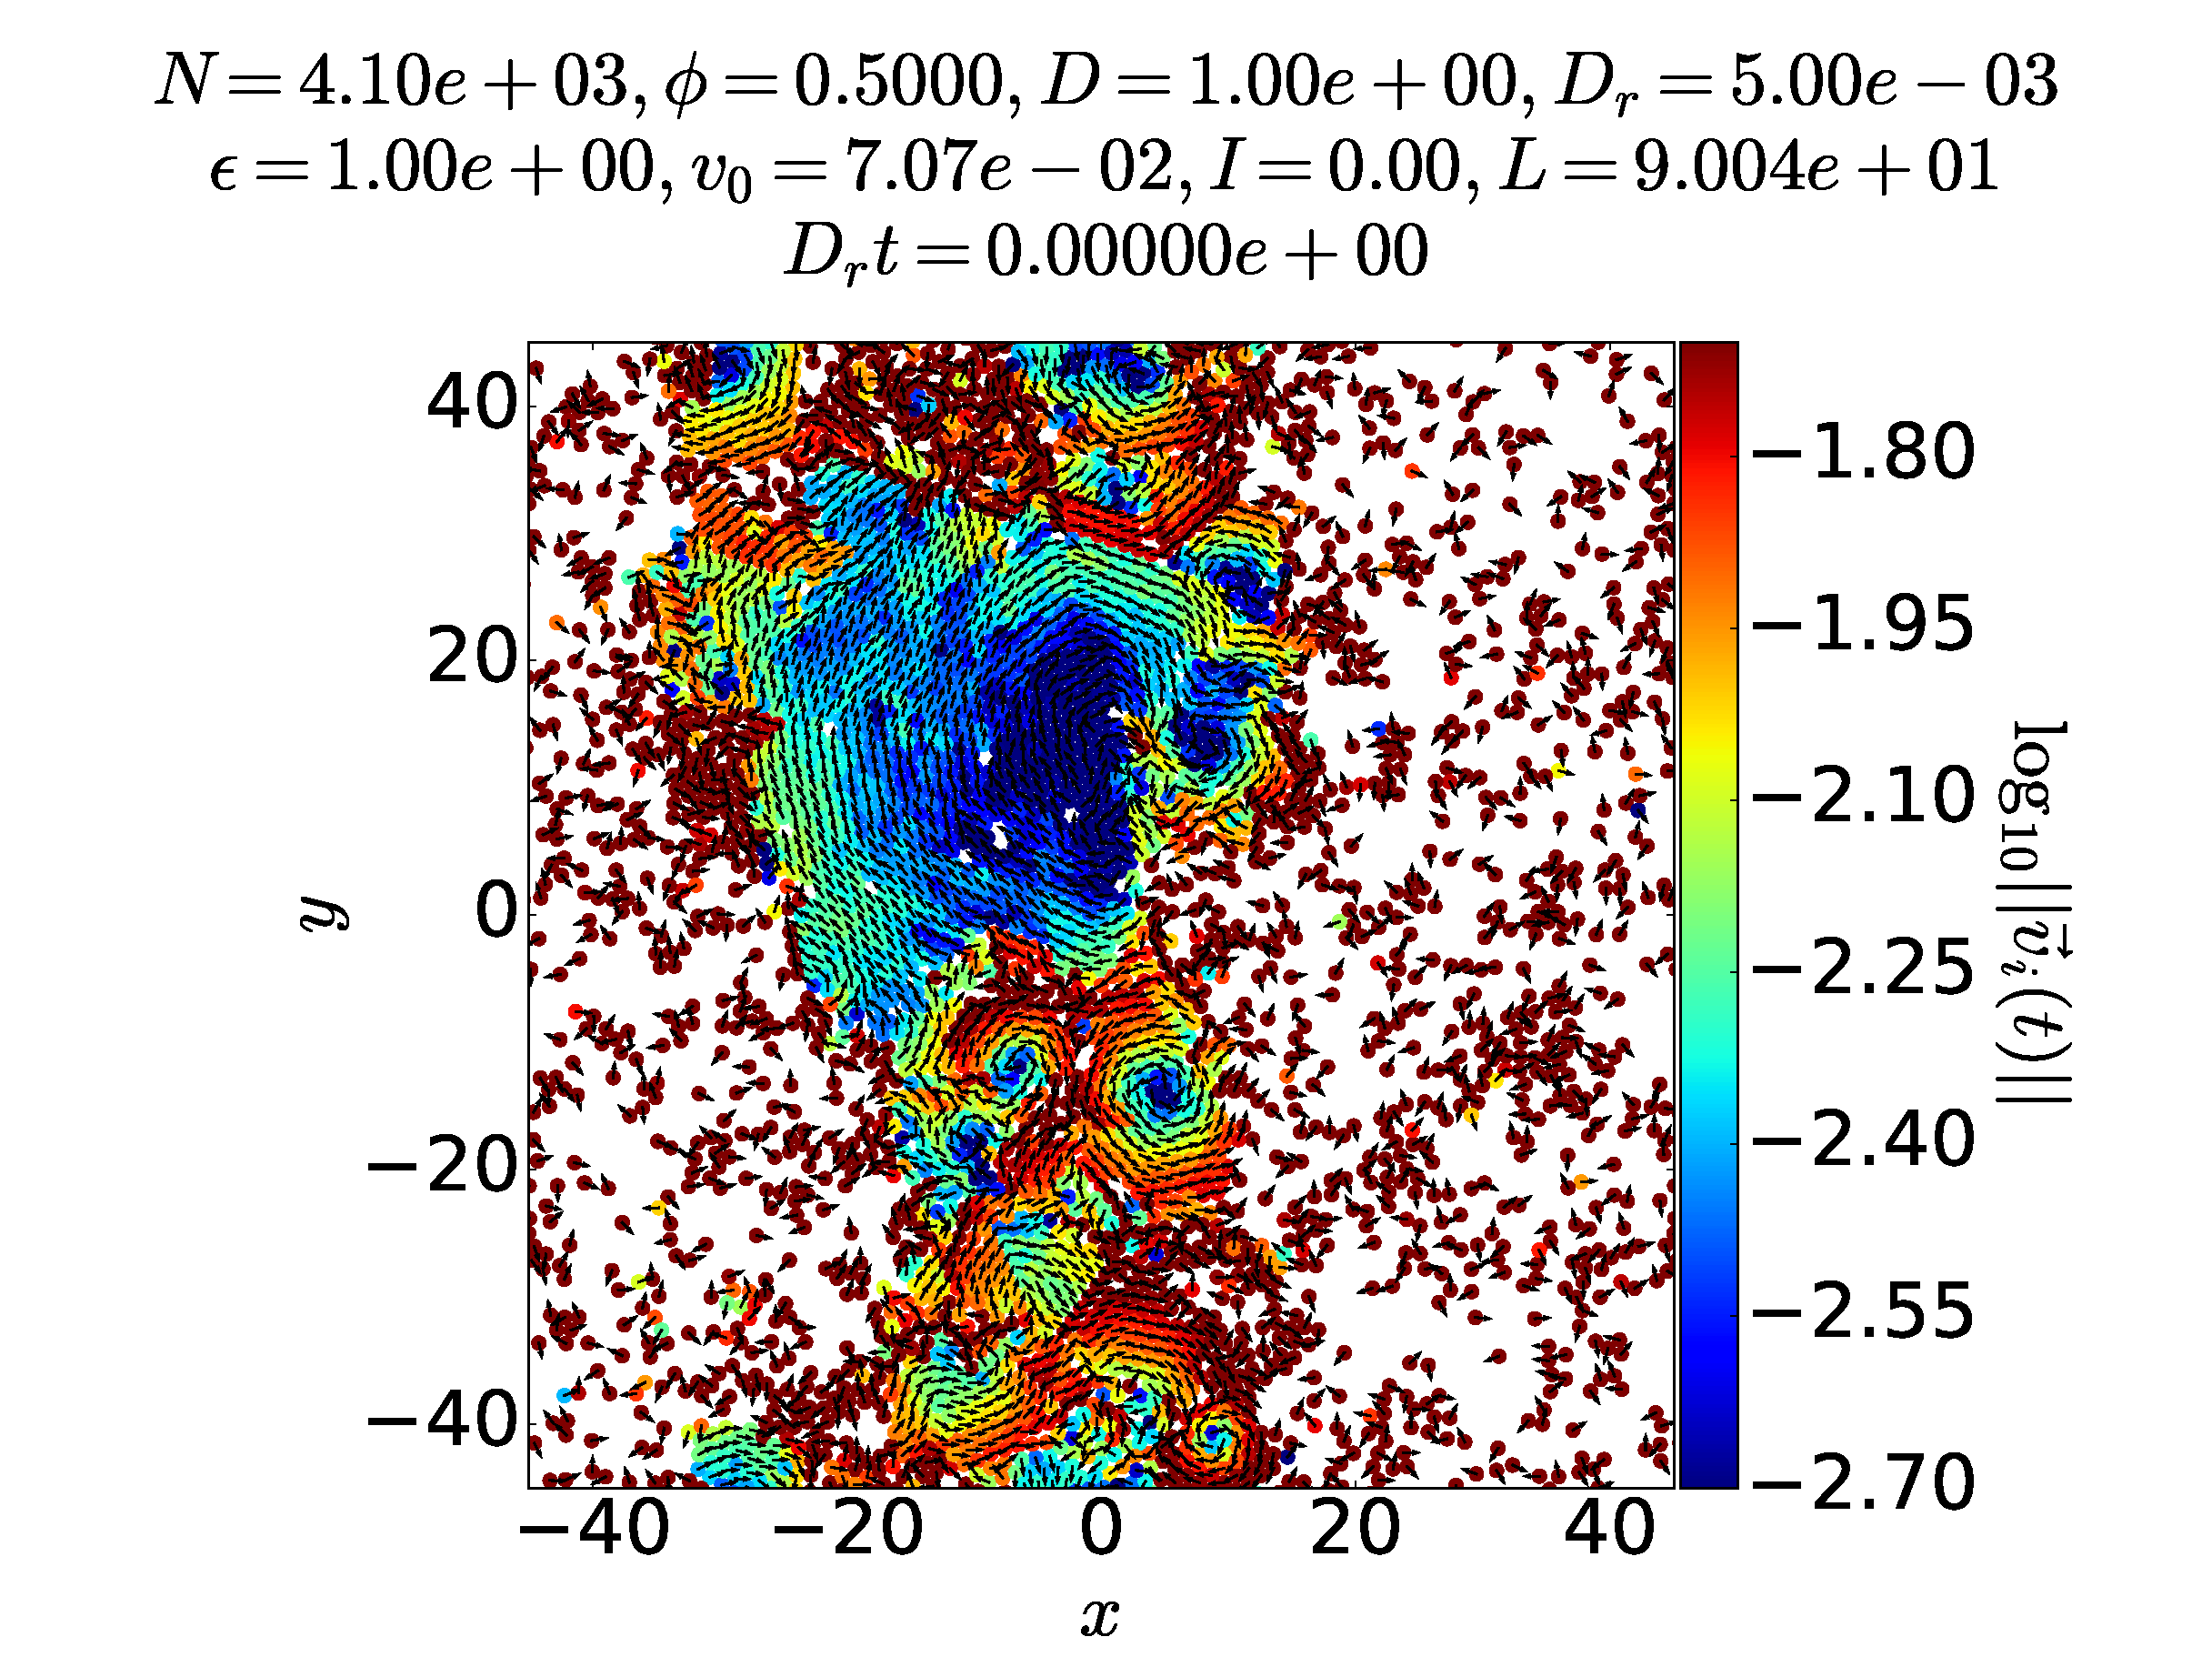
\includegraphics[width=0.45\textwidth]{No4096_Fl1000_Vl0000_Tl1000_Ri5000_Dk5000_EL3000.velo.eps}
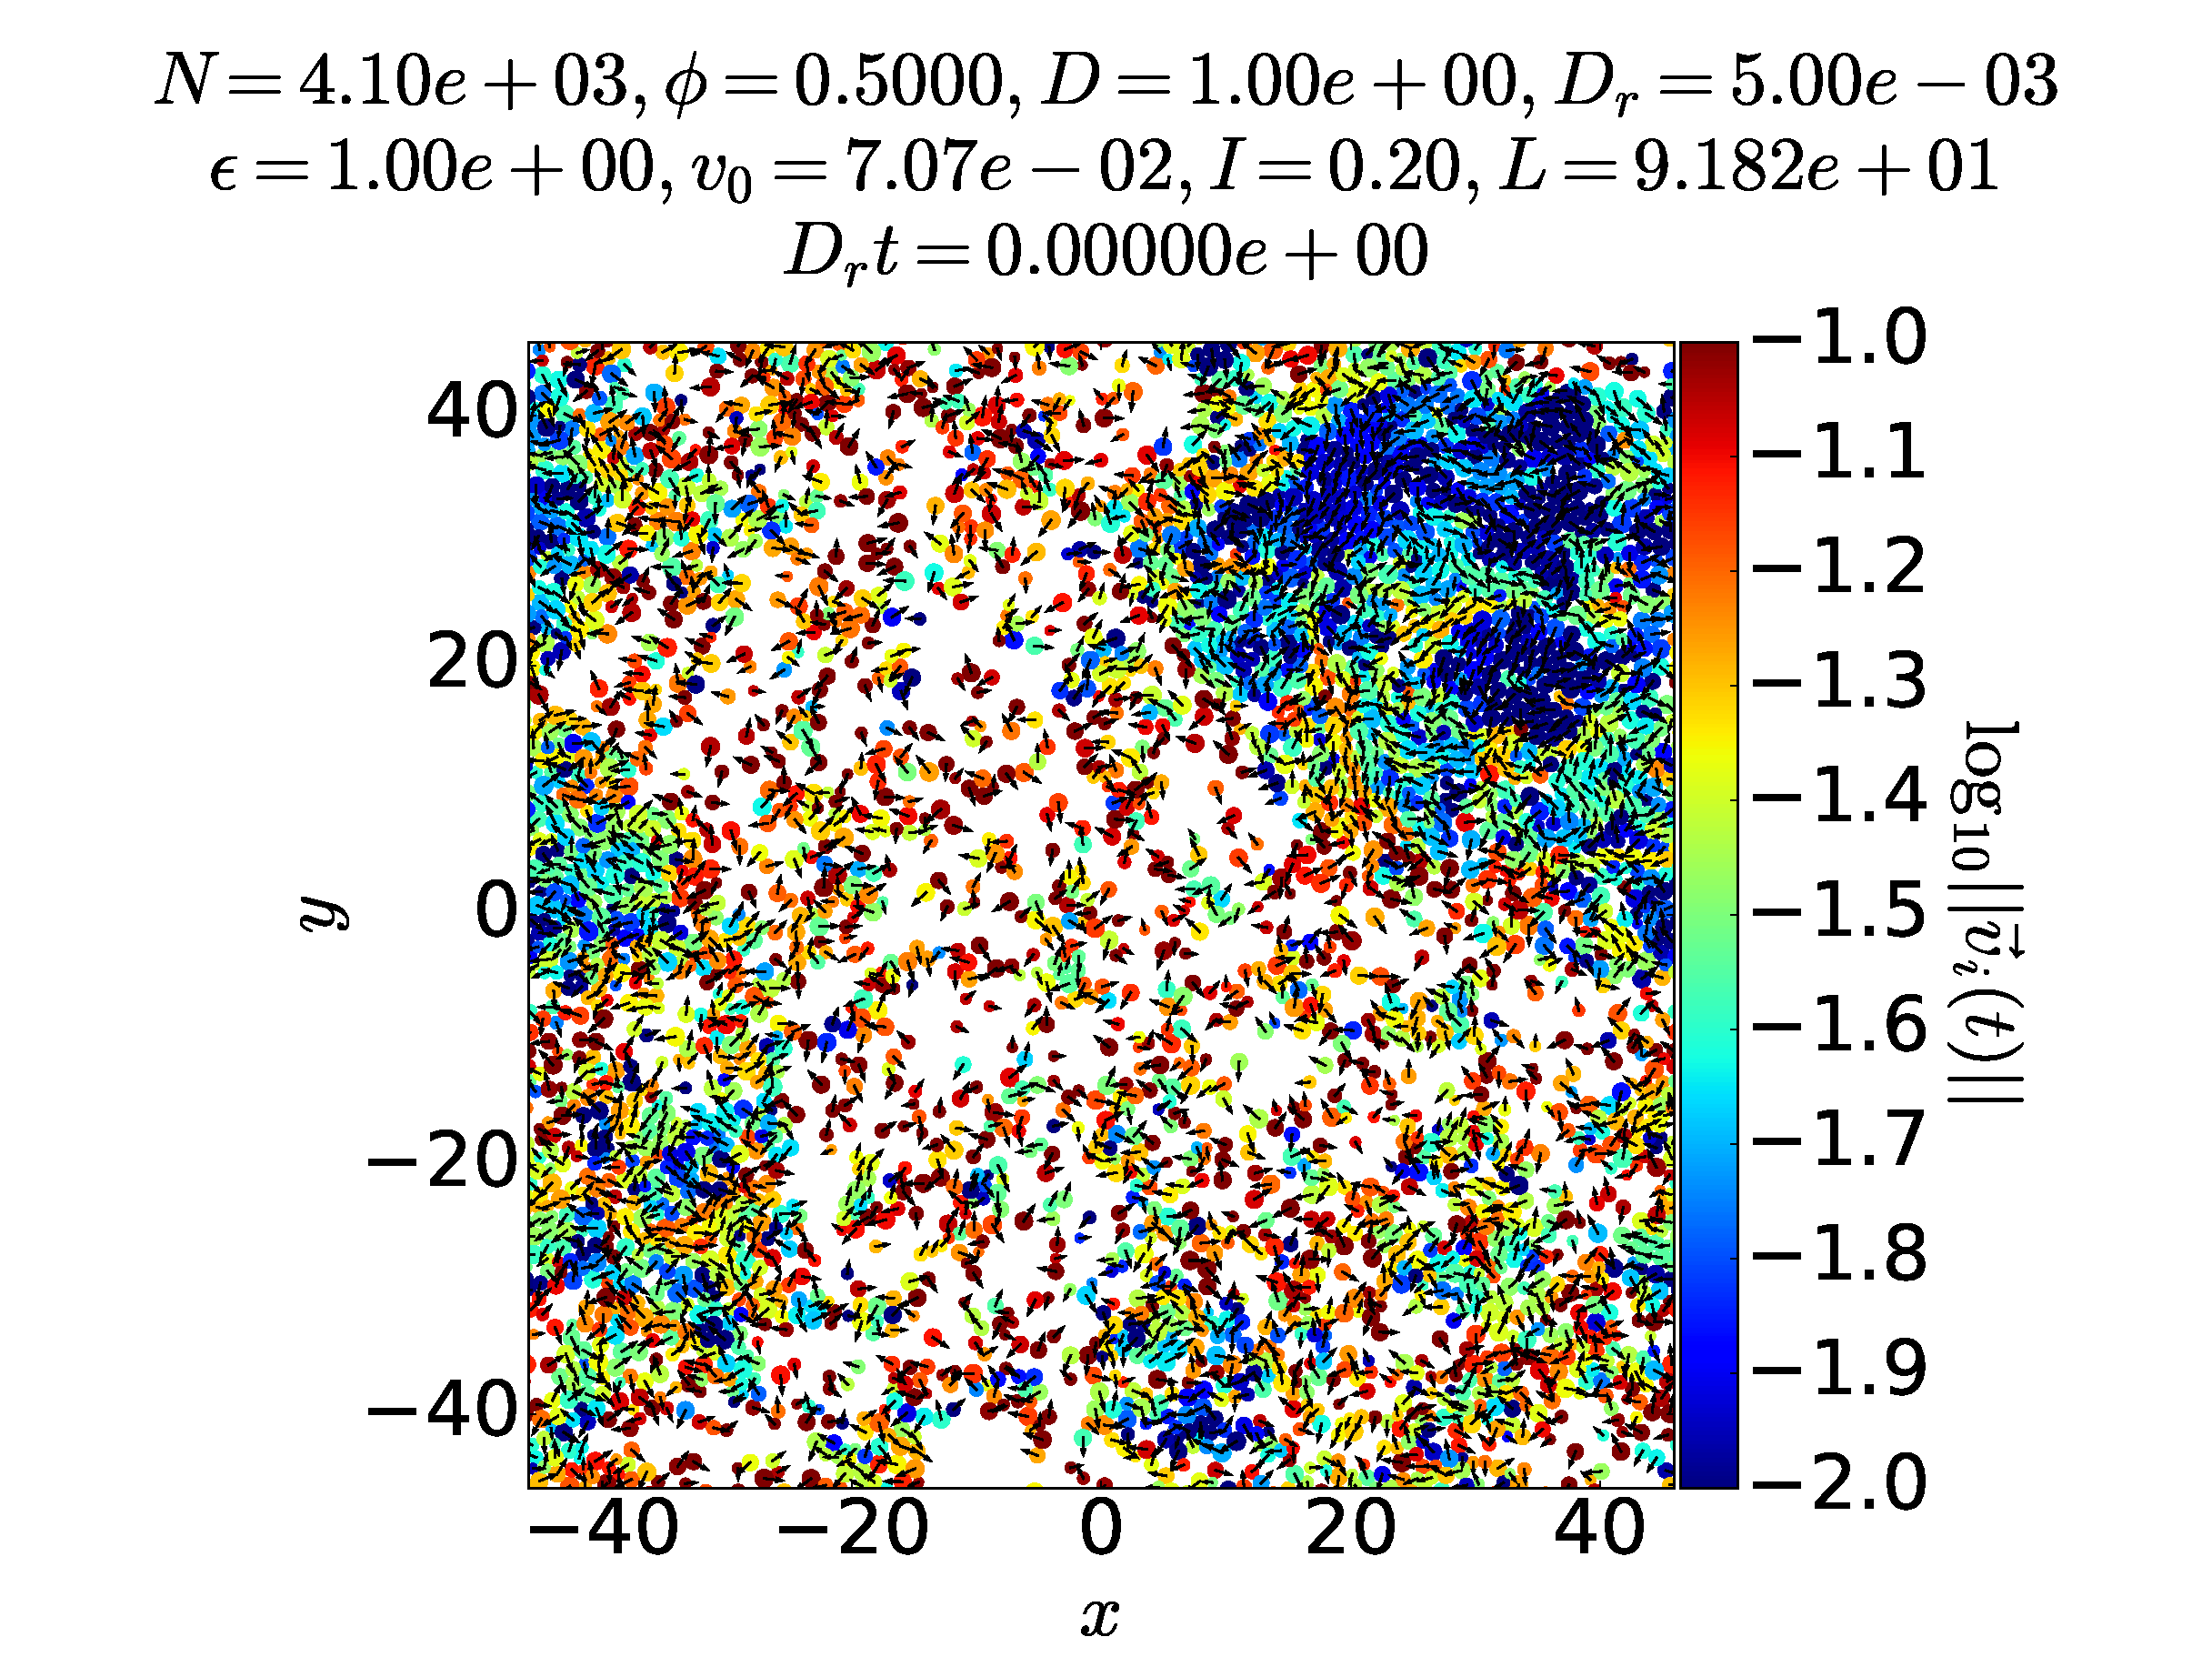
\includegraphics[width=0.45\textwidth]{No4096_Fl1000_Vl0000_Tl1000_Ri5000_Dk5000_El2000.velo.eps}
\caption{Velocity maps of AOUPs at packing fraction $\phi = 0.50$ and persistence time $D_r^{-1} = 200$, with polydispersity index {\bf (left)} $I = 0$ {\bf (right)} $I = 0.2$.}
\end{figure}

\footfullcitenomark{martin2020statistical}
\footfullcitenomark{berthier2017active}

\end{frame}

\begin{frame}{Model}

$N$ AOUPs with evolution
\begin{eqnarray}
\dot{\boldsymbol{r}}_i = -\nabla_i U_{\rm WCA} + \boldsymbol{p}_i\\
\dot{\boldsymbol{p}}_i = - D_r \boldsymbol{p}_i + \sqrt{2 D D_r^2} \boldsymbol{\eta}_i
\end{eqnarray}
with $\left<\eta^{\alpha}_i(t)\eta^{\beta}_j(t^{\prime})\right> = \delta_{\alpha\beta} \delta_{ij} \delta(t - t^{\prime})$ such that
\begin{equation}
\left<\boldsymbol{p}_i(t) \cdot \boldsymbol{p}_j(t^{\prime})\right> = 2 \delta_{ij} D D_r e^{-D_r |t - t^{\prime}|}
\end{equation}
$l_p = \sqrt{D/D_r}$, and $\tau_p = D_r^{-1} \to 0 \equiv$ Brownian system at $T = D$.\\
\mbox{}\\

Packing fraction and polydispersity index
\begin{eqnarray}
\phi = \frac{1}{L^2} \sum_{i=1}^N \frac{\pi (\sigma_i 2^{1/6})^2}{4}\\
I = \frac{\sqrt{\left<\sigma_i^2\right> - \left<\sigma_i\right>^2}}{\left<\sigma_i\right>}
\end{eqnarray}
and we fix $I = 0.2$ from a uniform distribution.

\end{frame}

\section{Structural relaxation}

\begin{frame}{Effective diffusion constant}

\begin{figure}
\centering
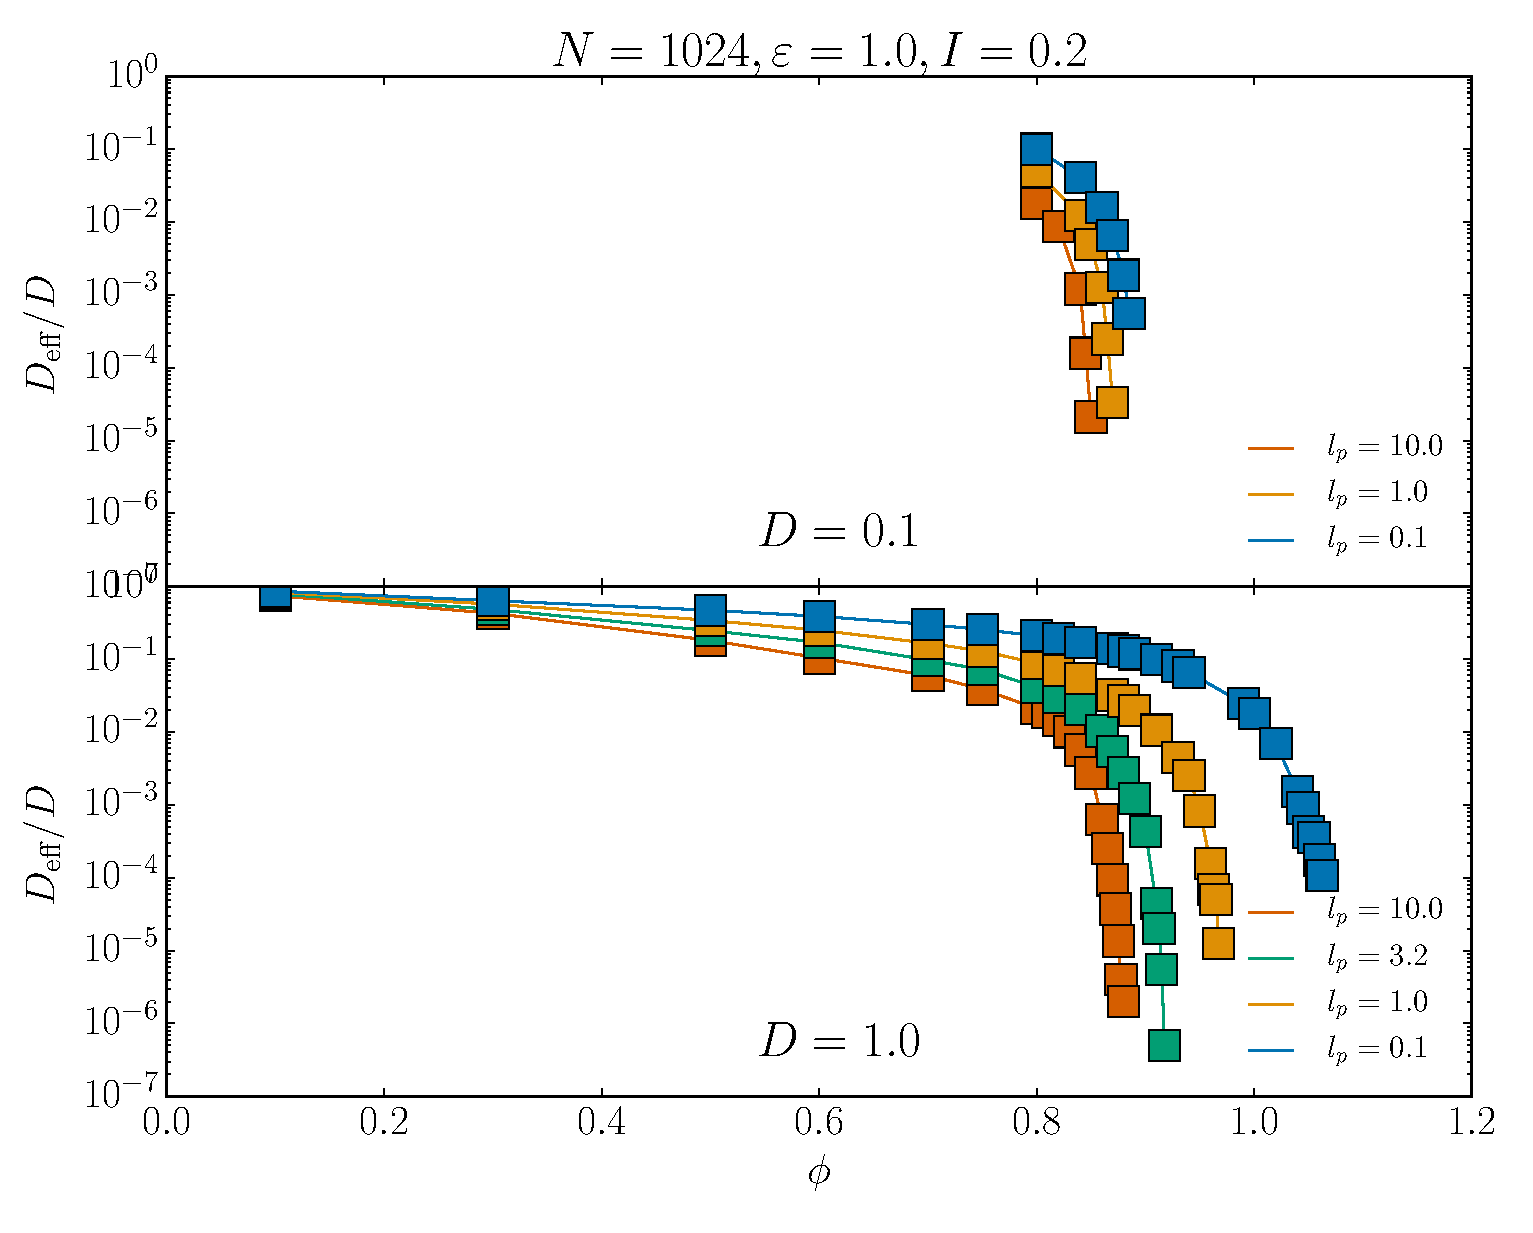
\includegraphics[width=0.45\textwidth]{Deff.eps}
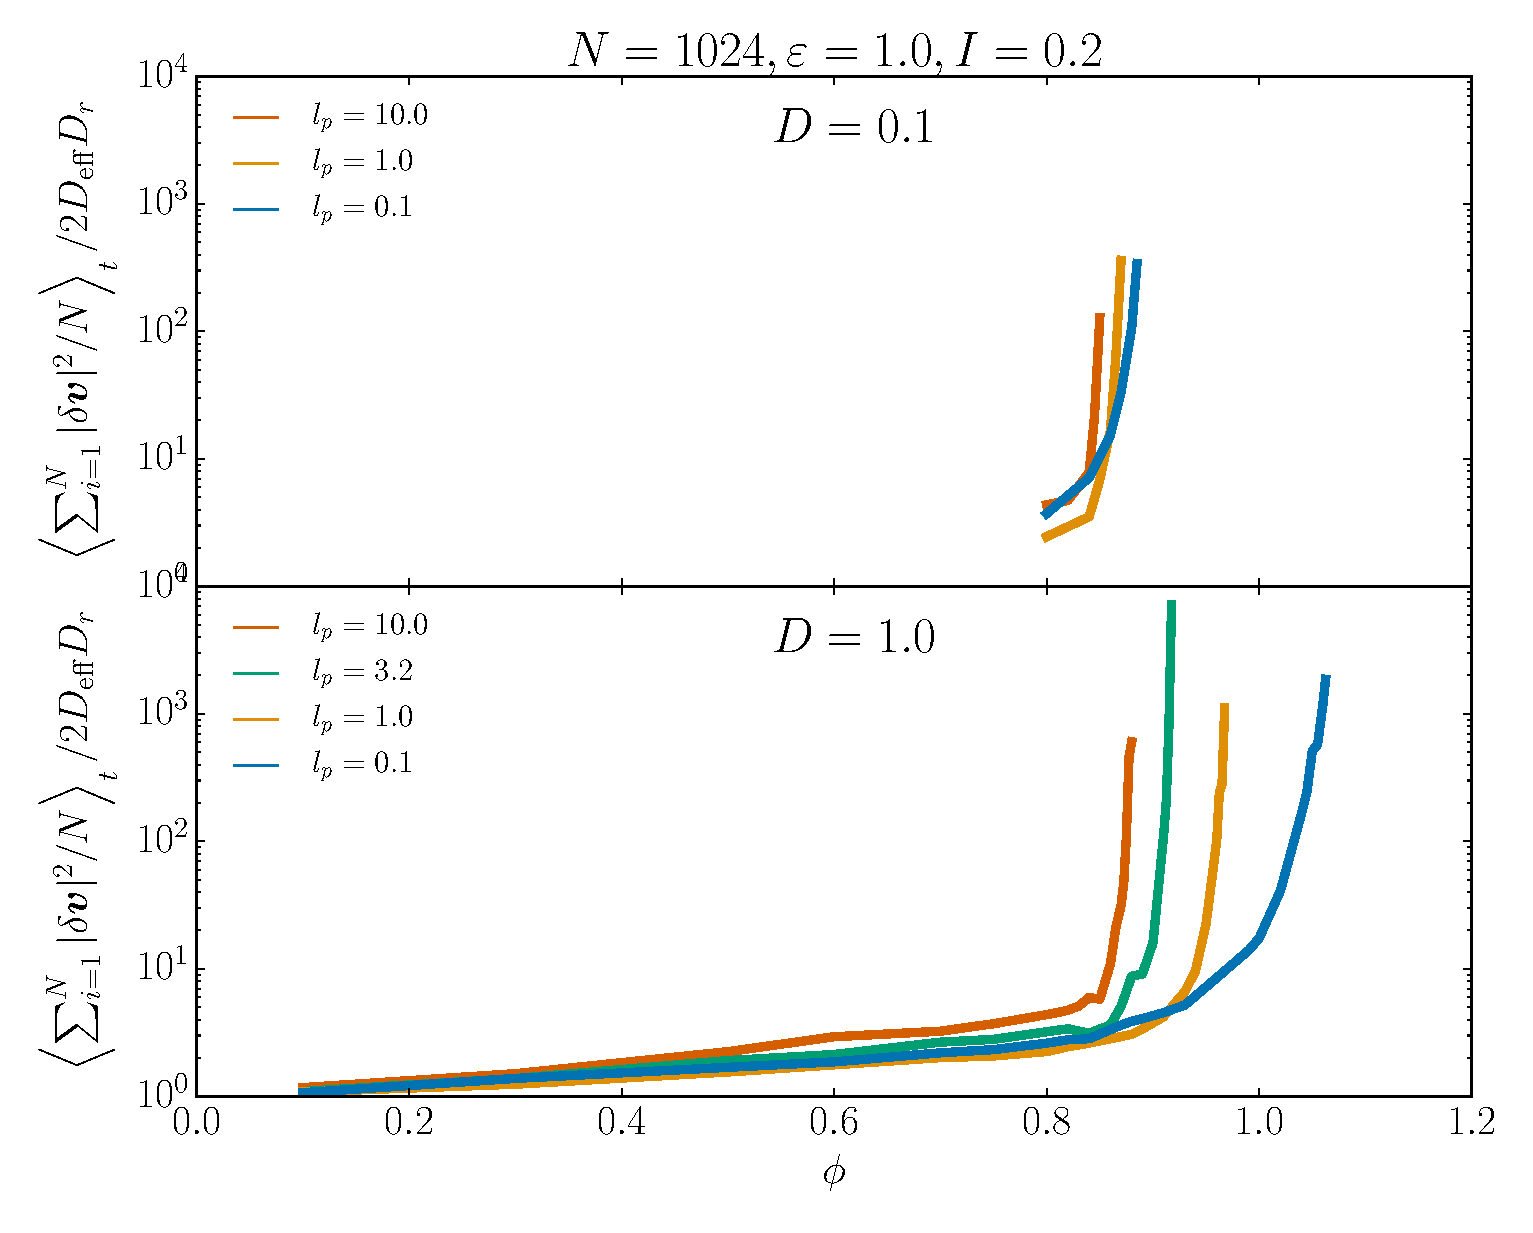
\includegraphics[width=0.45\textwidth]{DeffV2.eps}
\caption{ Effective diffusion constant $D_{\mathrm{eff}} = \lim_{\Delta t \to \infty} \left<|\Delta\boldsymbol{r}_i(t, t + \Delta t)|^2\right>_{i, t}/4\Delta t$ and ratio with kinetic energy $\left<\sum_{i=1}^N |\boldsymbol{v}_i(t)|^2/N\right>_t$.}
\end{figure}

\footfullcitenomark{janssen2019active}

\end{frame}

\begin{frame}{Pair distribution function}

\begin{figure}
\centering
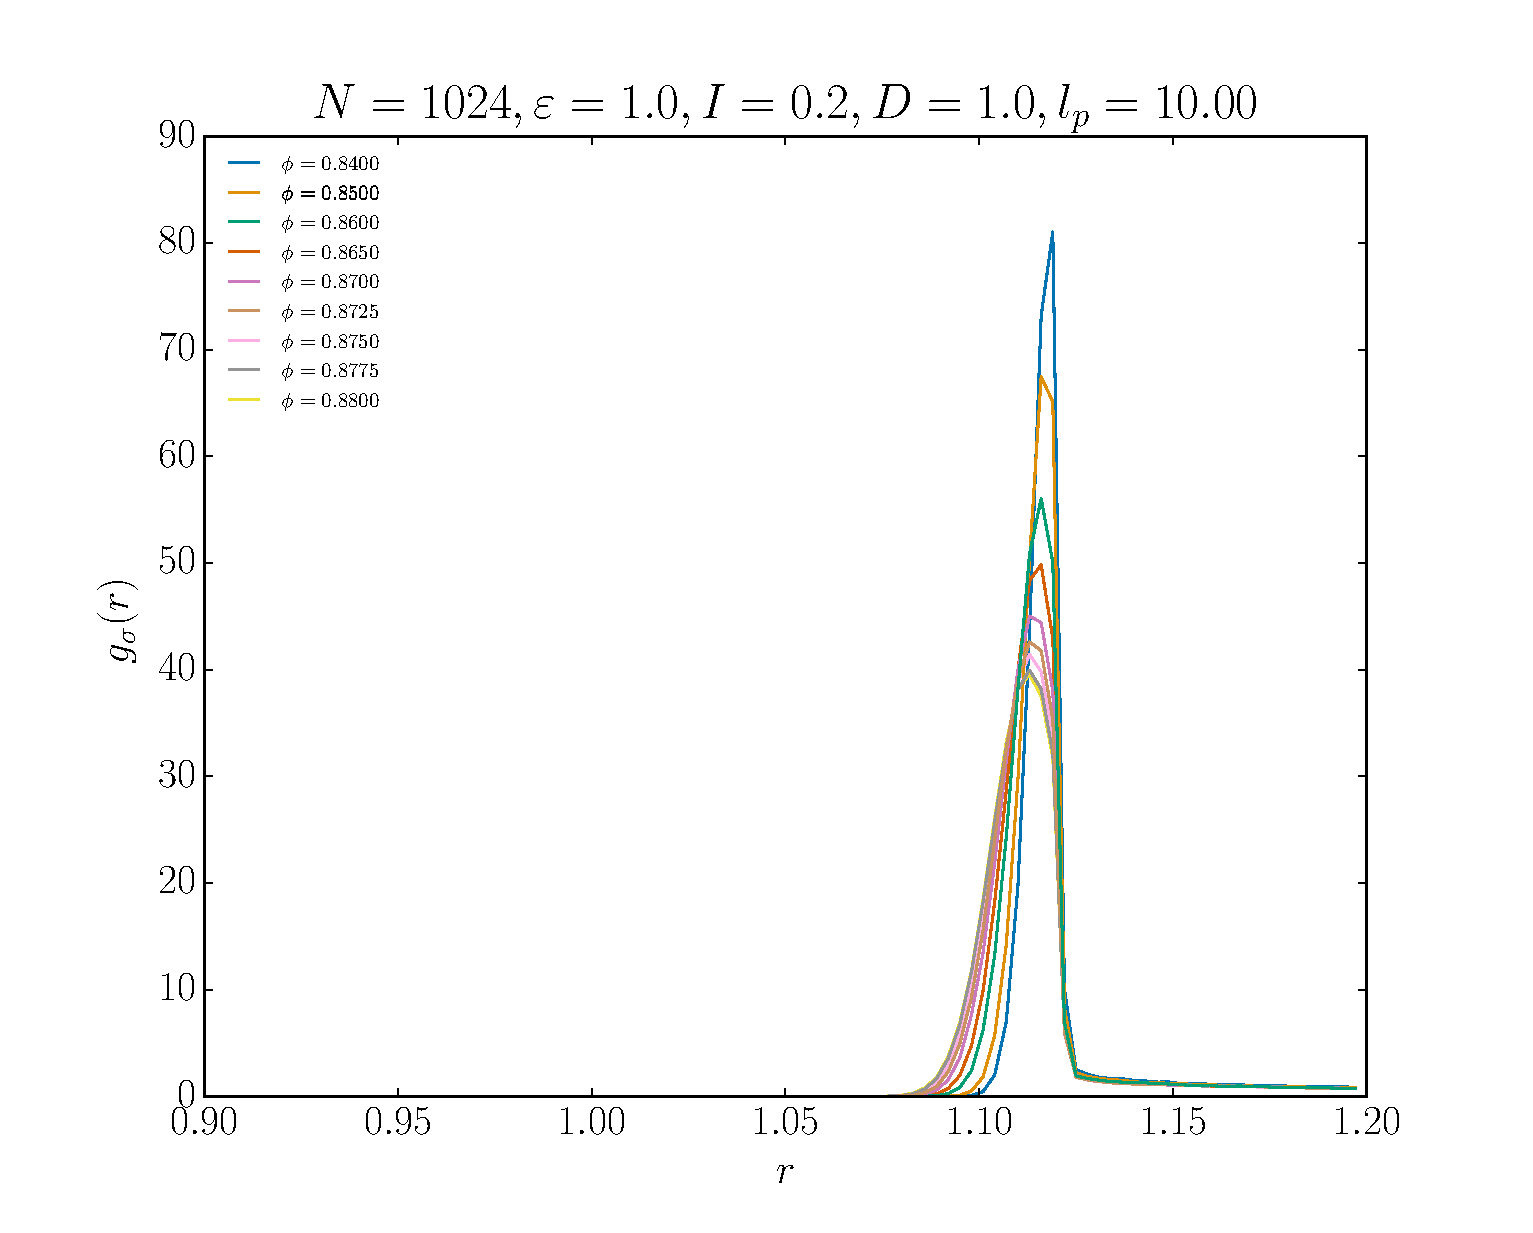
\includegraphics[width=0.35\textwidth]{g_No1024_Tl1000_Rj1000.eps}
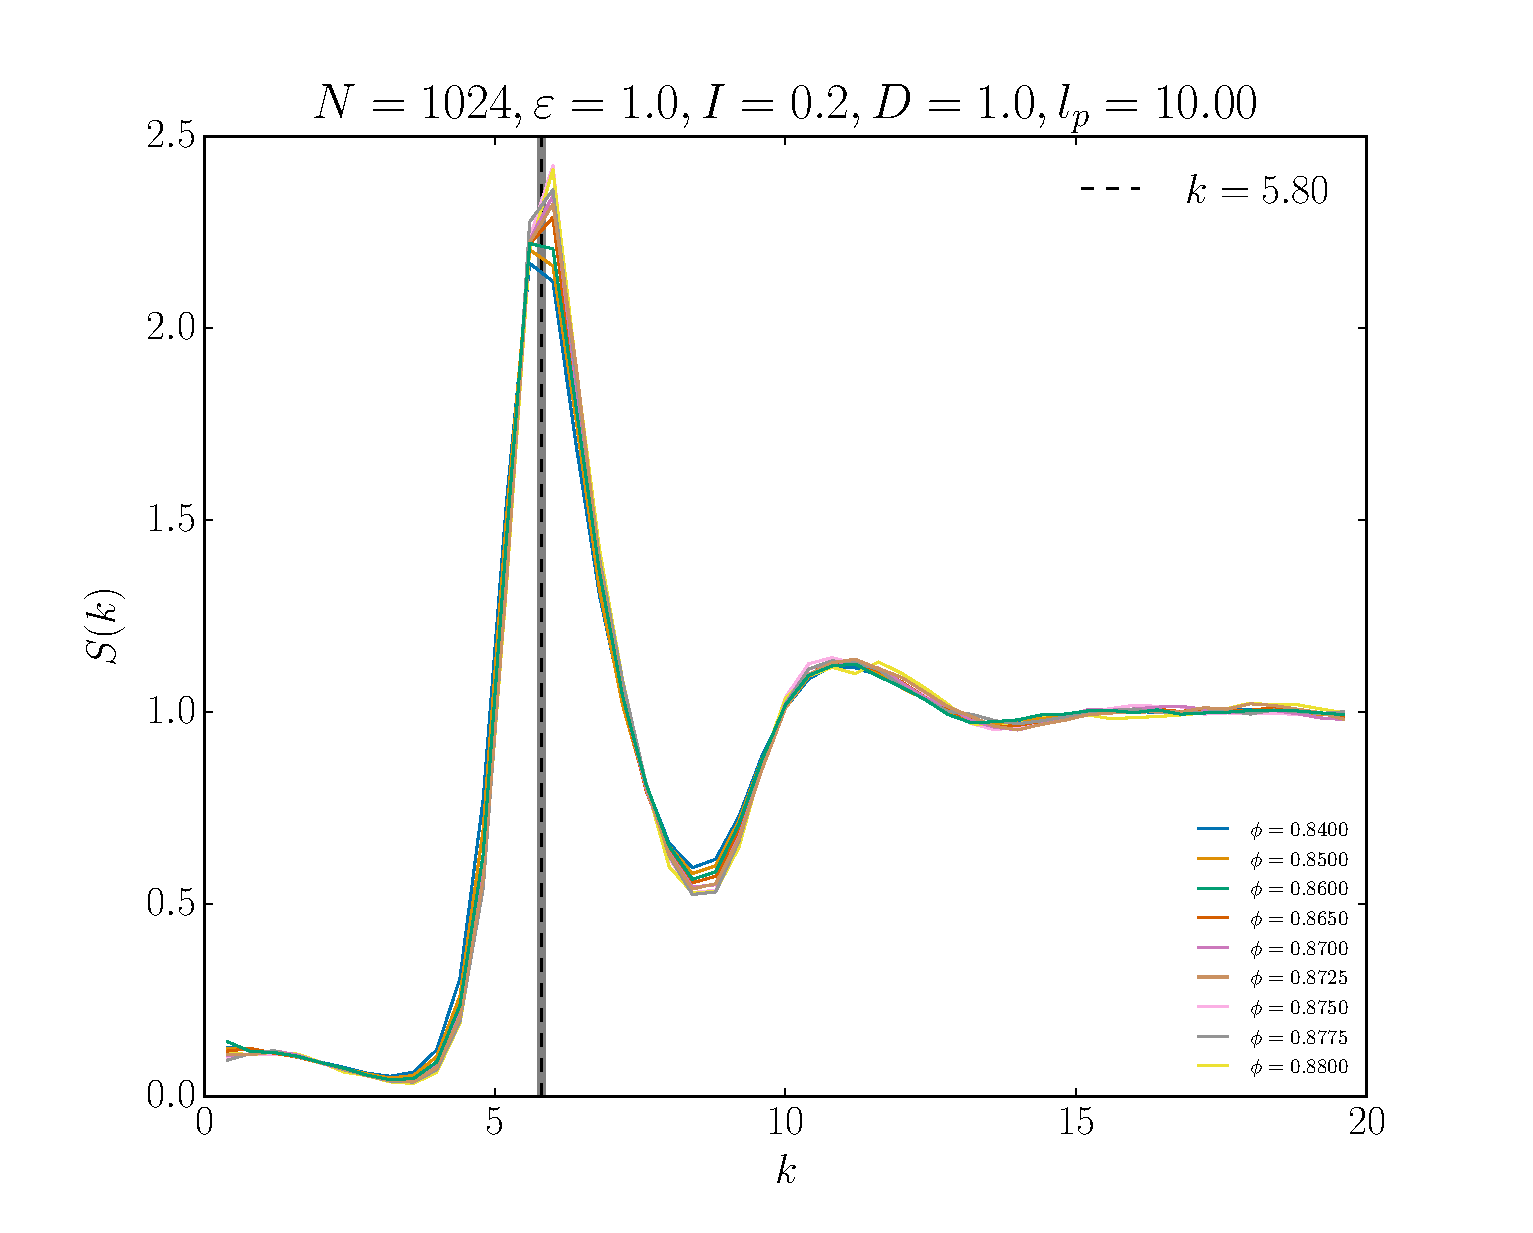
\includegraphics[width=0.35\textwidth]{S_No1024_Tl1000_Rj1000.eps}\\
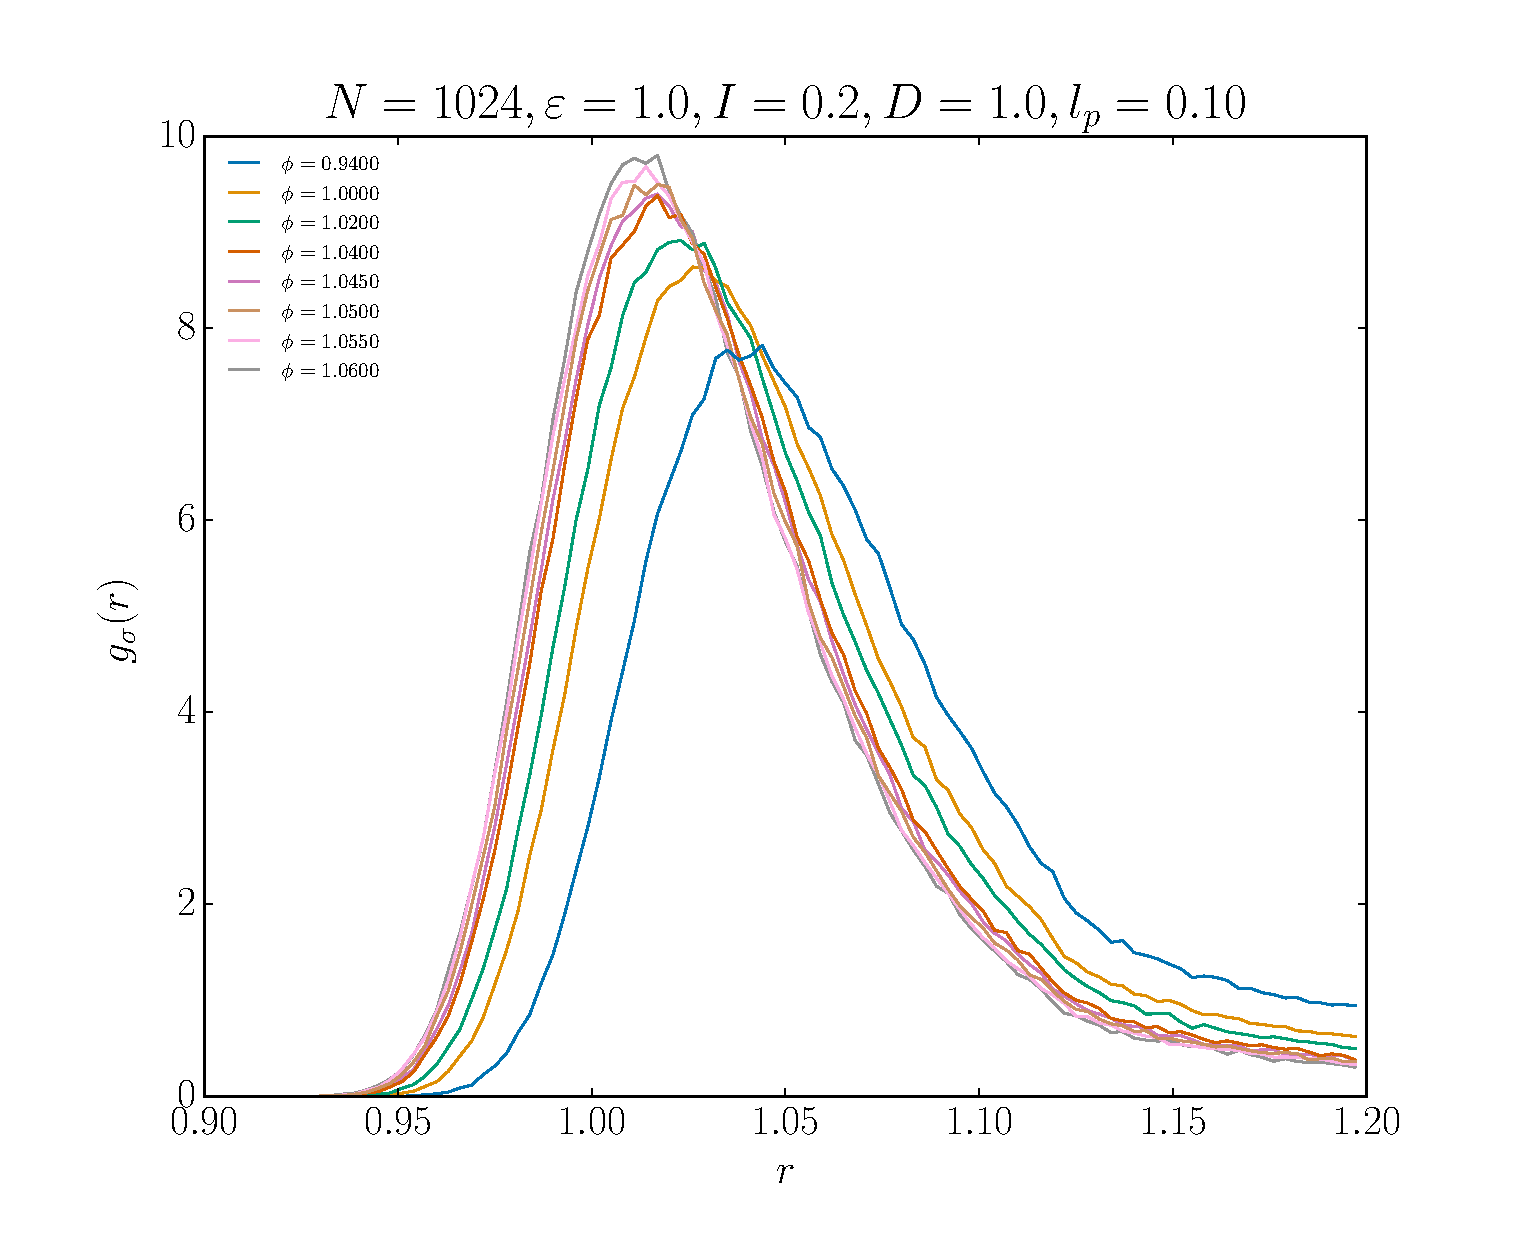
\includegraphics[width=0.35\textwidth]{g_No1024_Tl1000_Rn1000.eps}
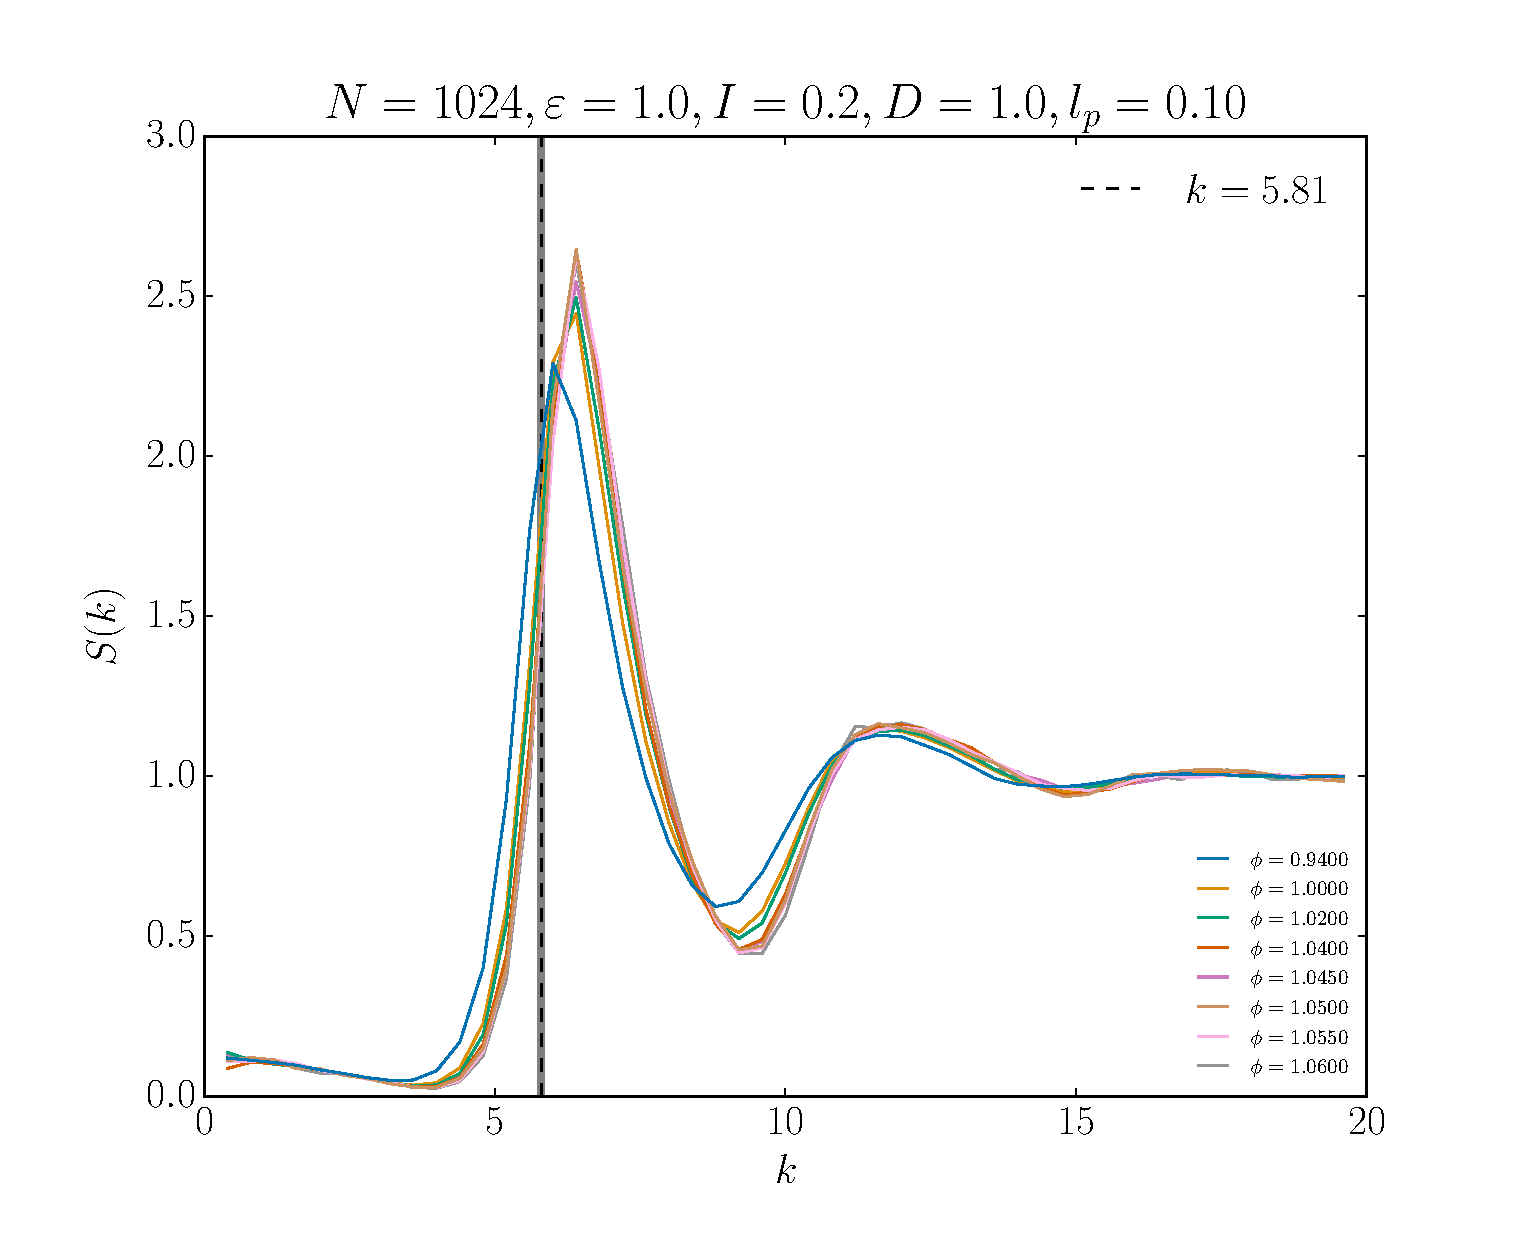
\includegraphics[width=0.35\textwidth]{S_No1024_Tl1000_Rn1000.eps}
\caption{{\bf (left)} Diameter-relative pair distribution function $g_{\sigma}$ and {\bf(right)} structure factor $S(k) = \left<|\rho_{\boldsymbol{k}}|^2\right>$, at {\bf (top)} $\tau_p = 10^2$ and {\bf (bottom)} $\tau_p = 10^{-2}$.}
\end{figure}

\end{frame}

\begin{frame}{MSD and scattering function}

\begin{figure}
\centering
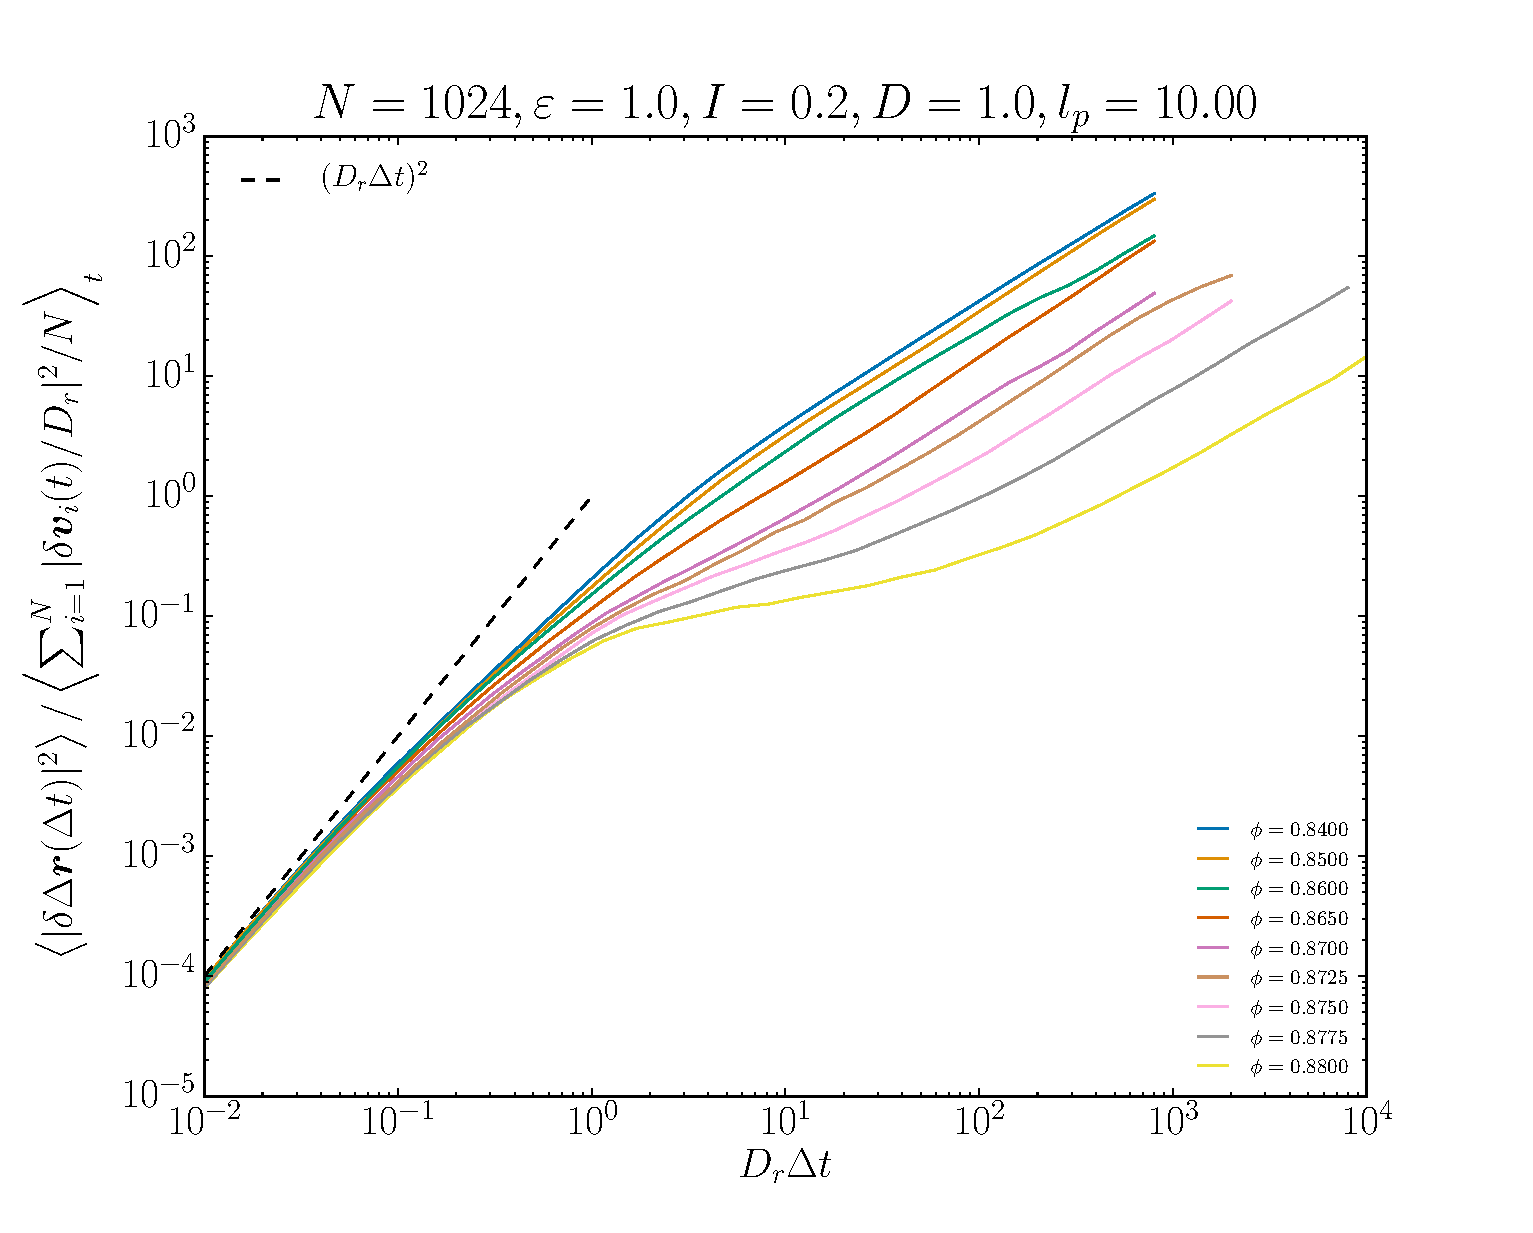
\includegraphics[width=0.35\textwidth]{msdv2_No1024_Tl1000_Rj1000.eps}
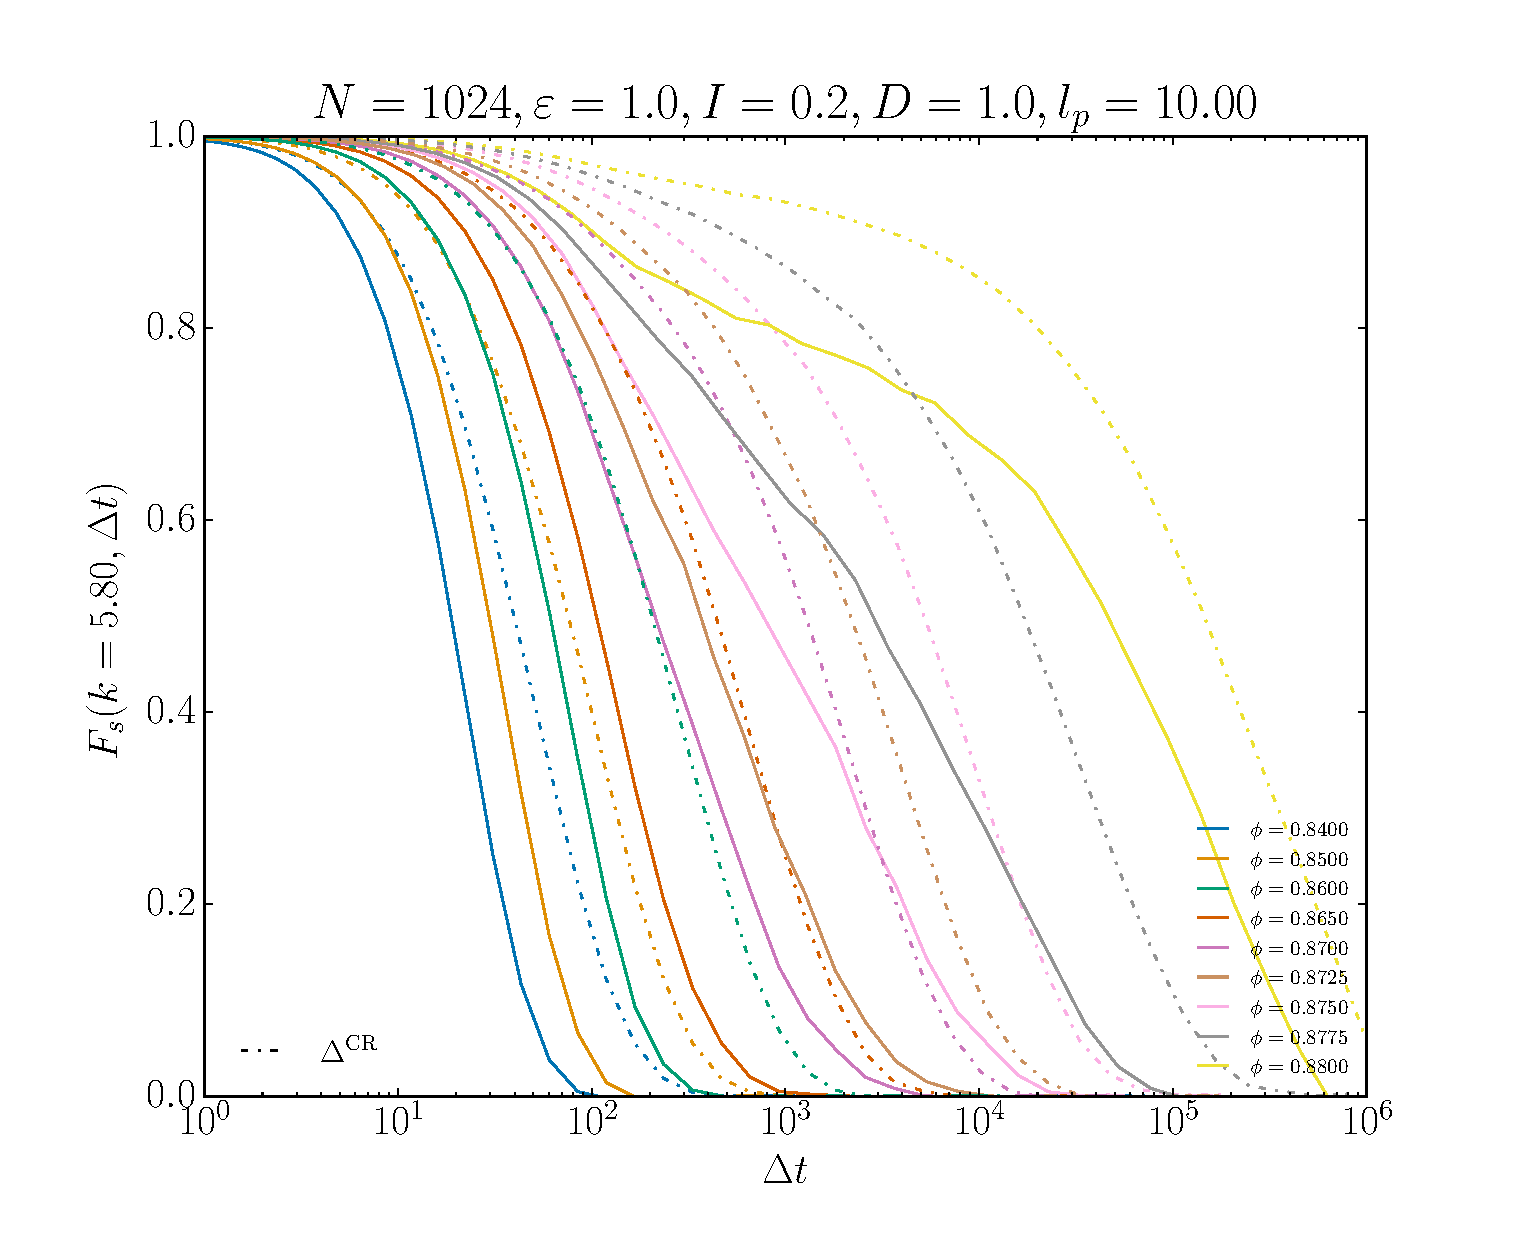
\includegraphics[width=0.35\textwidth]{Fs_No1024_Tl1000_Rj1000.eps}\\
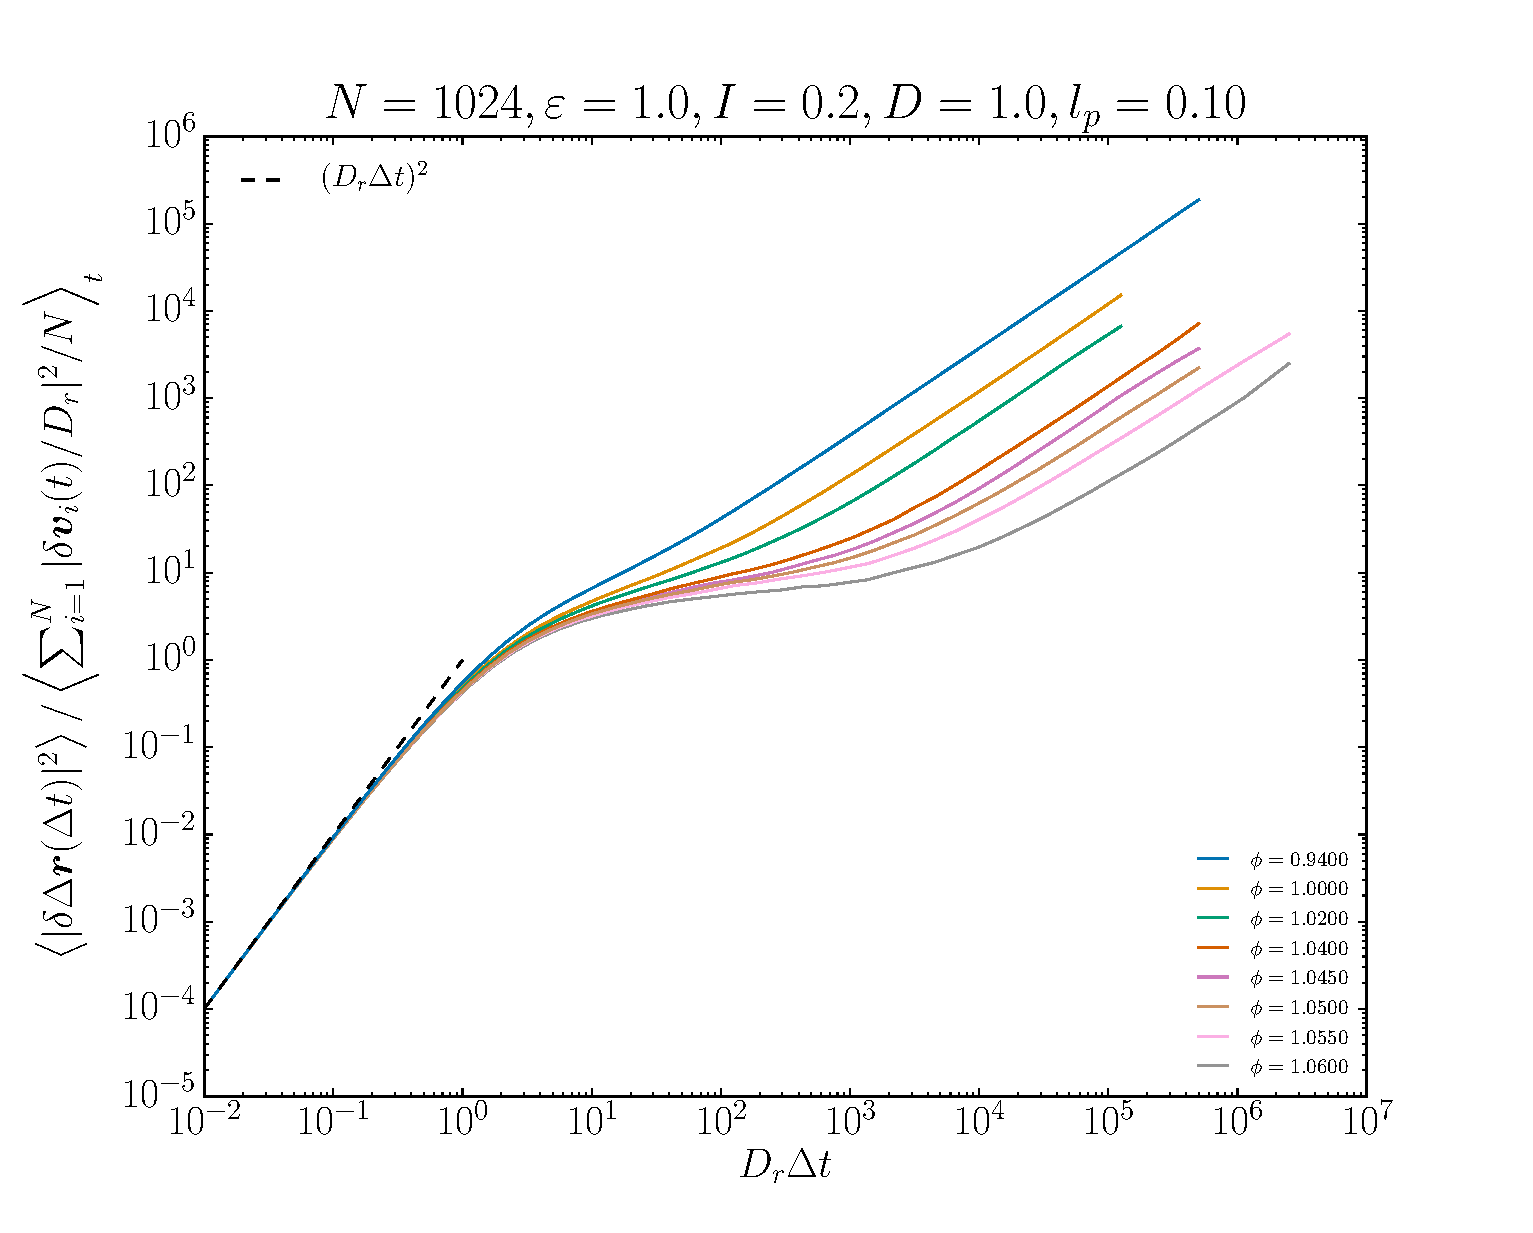
\includegraphics[width=0.35\textwidth]{msdv2_No1024_Tl1000_Rn1000.eps}
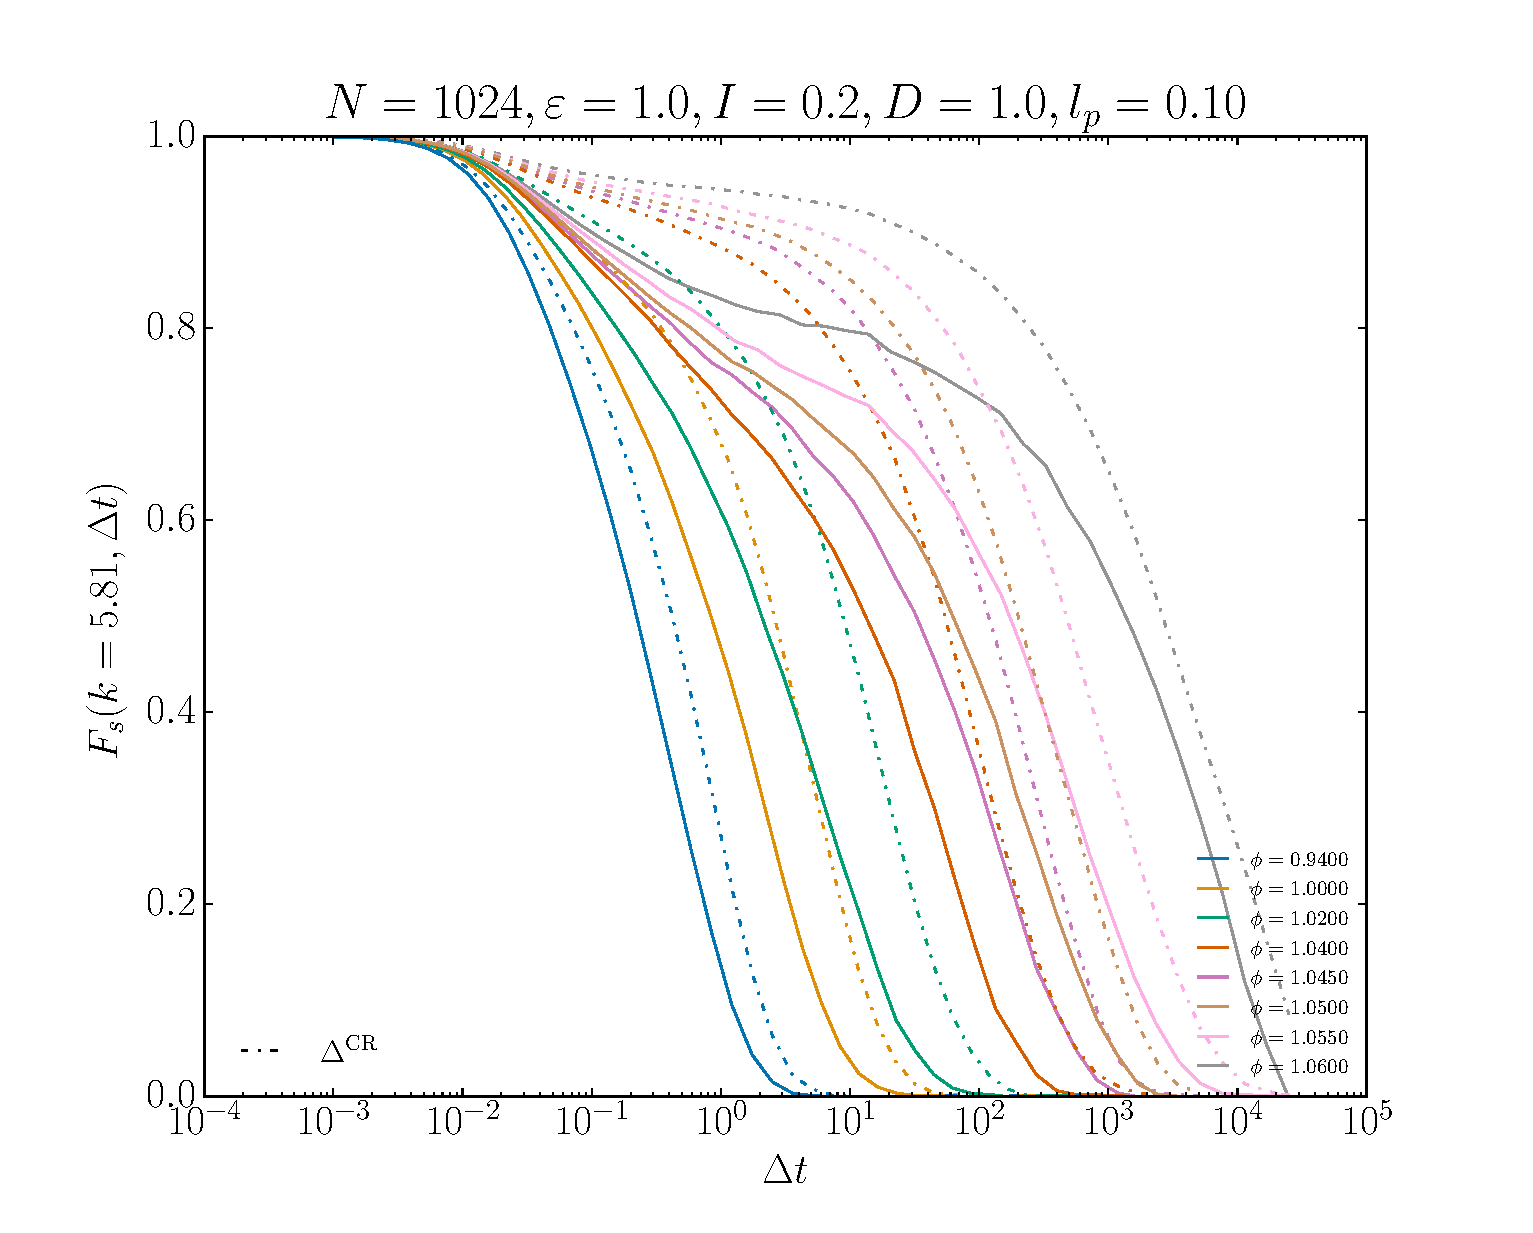
\includegraphics[width=0.35\textwidth]{Fs_No1024_Tl1000_Rn1000.eps}
\caption{{\bf (left)} Mean squared displacement rescaled by mean squared velocity and {\bf (right)} self-intermediate scattering function, at {\bf (top)} $\tau_p = 10^2$ and {\bf (bottom)} $\tau_p = 10^{-2}$.}
\end{figure}

\end{frame}

\begin{frame}{Overlap susceptibility}

\begin{equation}
\chi(\Delta t, a) = N \mathrm{Var}\left(\exp\left(-|\Delta \boldsymbol{r}_i(t, t + \Delta t)|^2/a^2\right)\right)_t
\end{equation}
\mbox{}\\

\begin{figure}
\centering
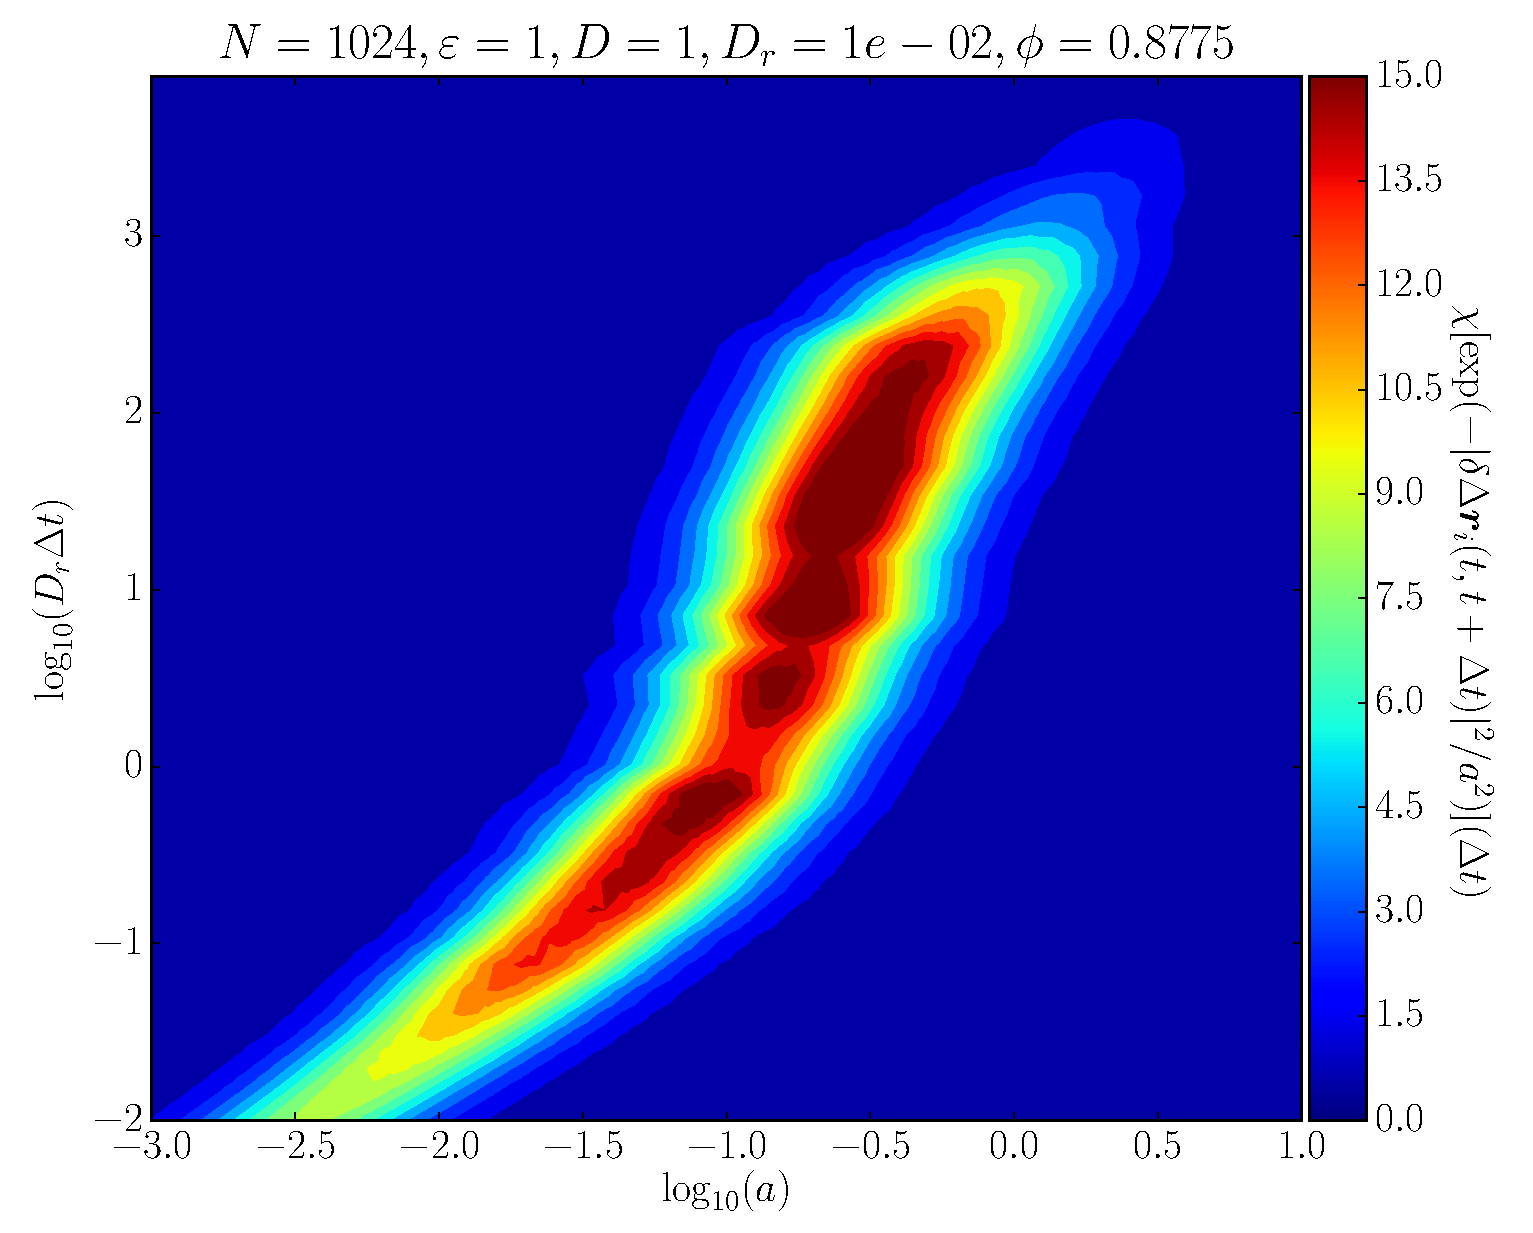
\includegraphics[width=0.45\textwidth]{No1024_Fl1000_Vl0000_Tl1000_Rj1000_Dk8775_El0000.datN.overlap.eps}
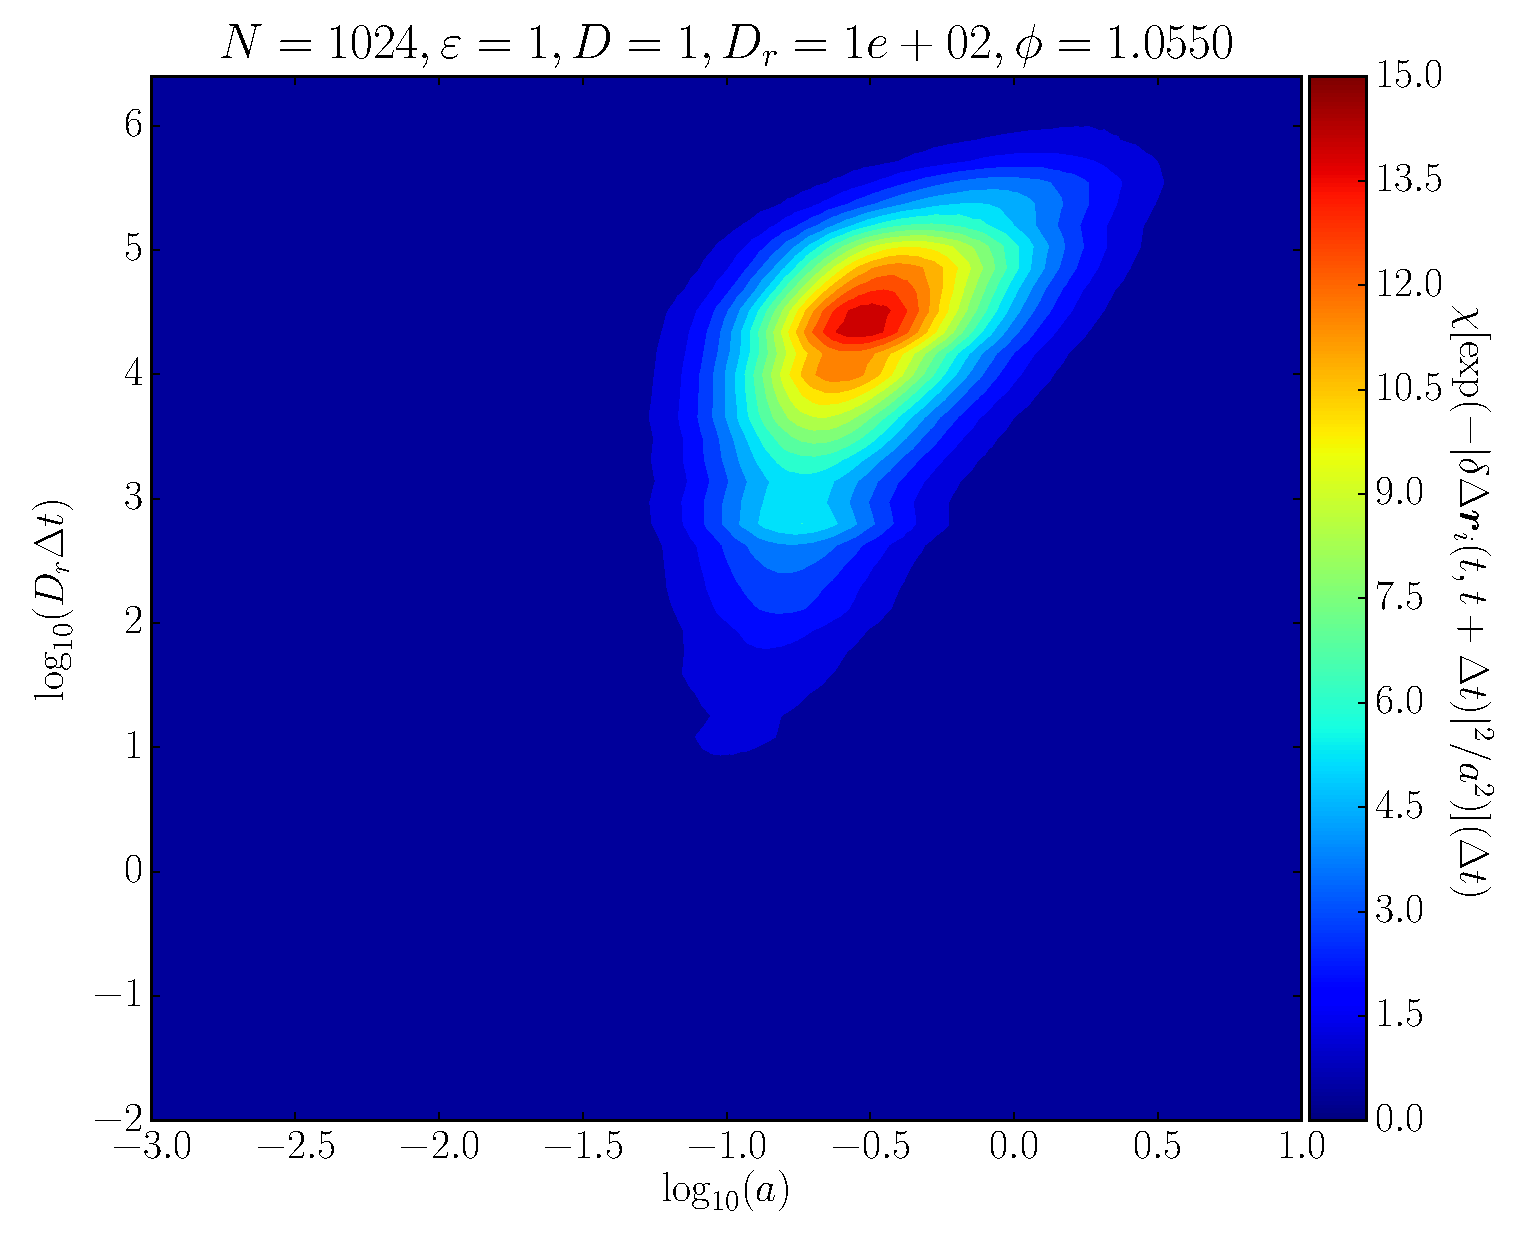
\includegraphics[width=0.45\textwidth]{No1024_Fl1000_Vl0000_Tl1000_Rn1000_Dl1055_El0000.datN.overlap.eps}
\caption{Overlap susceptibility $\chi$ at {\bf (left)} $\tau_p = 10^2$ and {\bf (right)} $\tau_p = 10^{-2}$.}
\end{figure}

\end{frame}

\section{Velocity correlations}

\begin{frame}{Velocity maps}

\begin{figure}
\centering
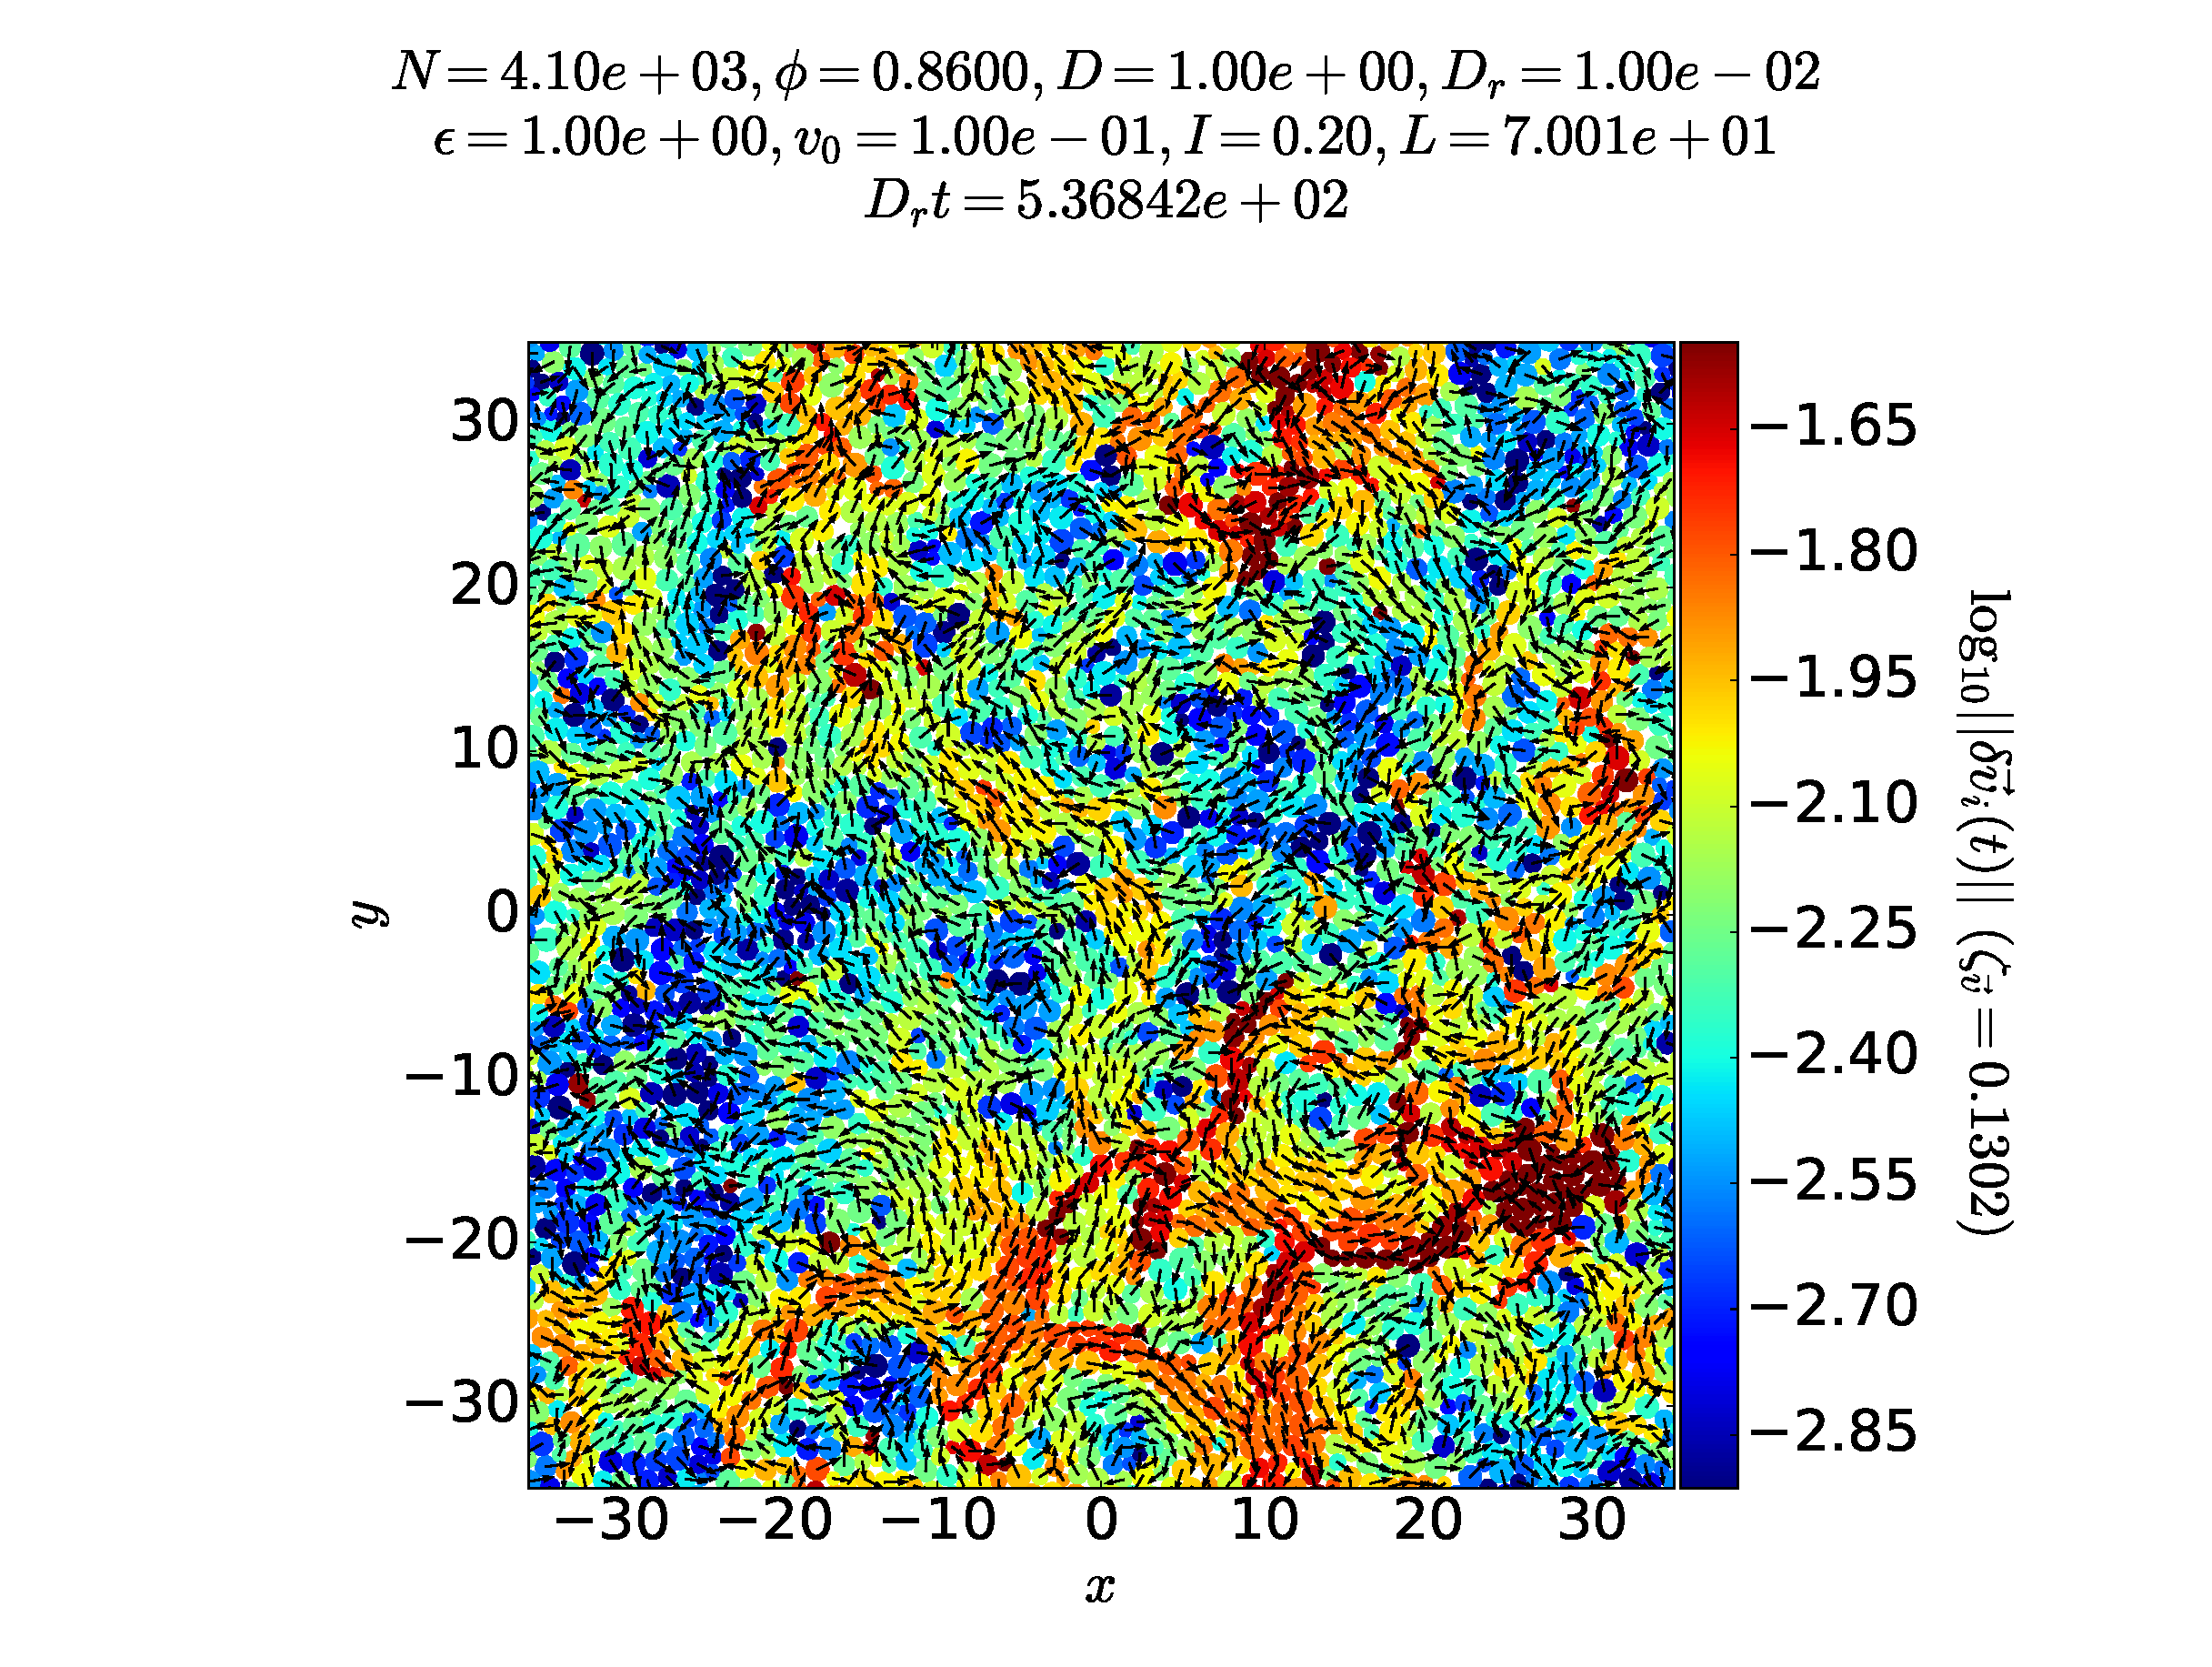
\includegraphics[width=0.49\textwidth]{No4096_Fl1000_Vl0000_Tl1000_Rj1000_Dk8600_El0000.velo.eps}
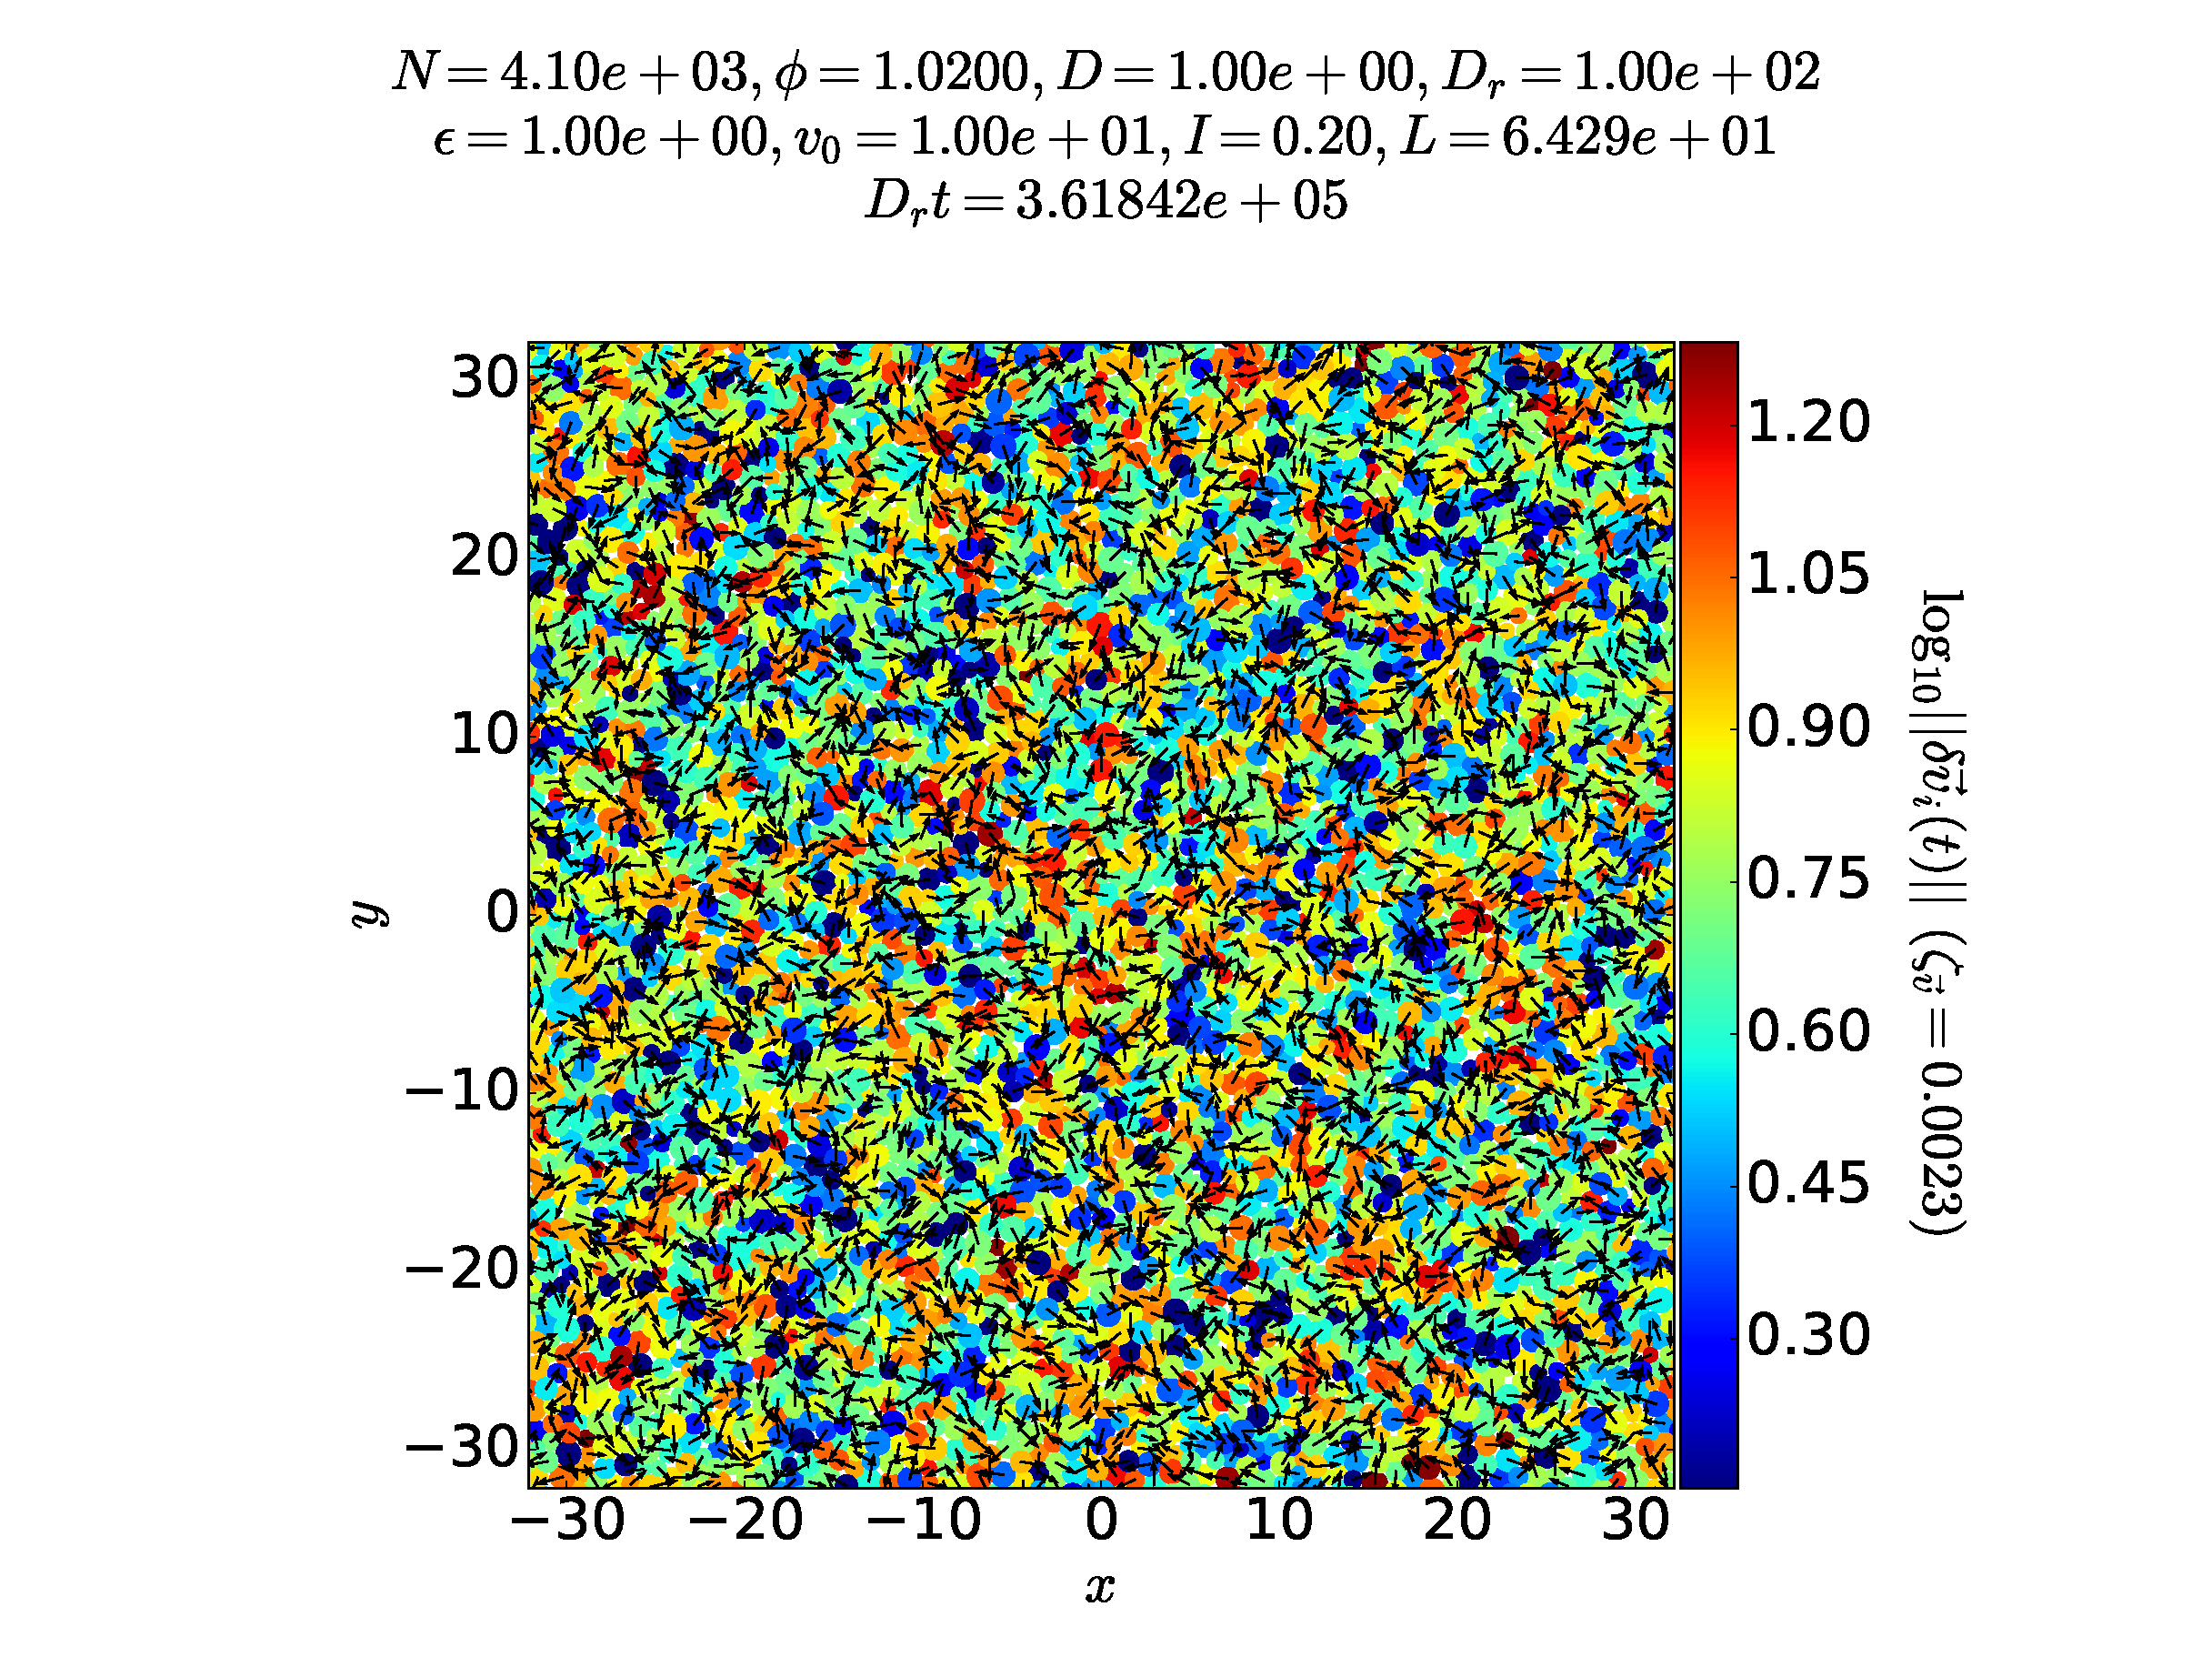
\includegraphics[width=0.49\textwidth]{No4096_Fl1000_Vl0000_Tl1000_Rn1000_Dl1020_El0000.velo.eps}
\caption{Velocity maps at {\bf (left)} $\tau_p = 10^2$ and {\bf (right)} $\tau_p = 10^{-2}$.}
\end{figure}

\footfullcitenomark{caprini2020hidden}

\end{frame}

\begin{frame}{Velocity correlations}

\begin{figure}
\centering
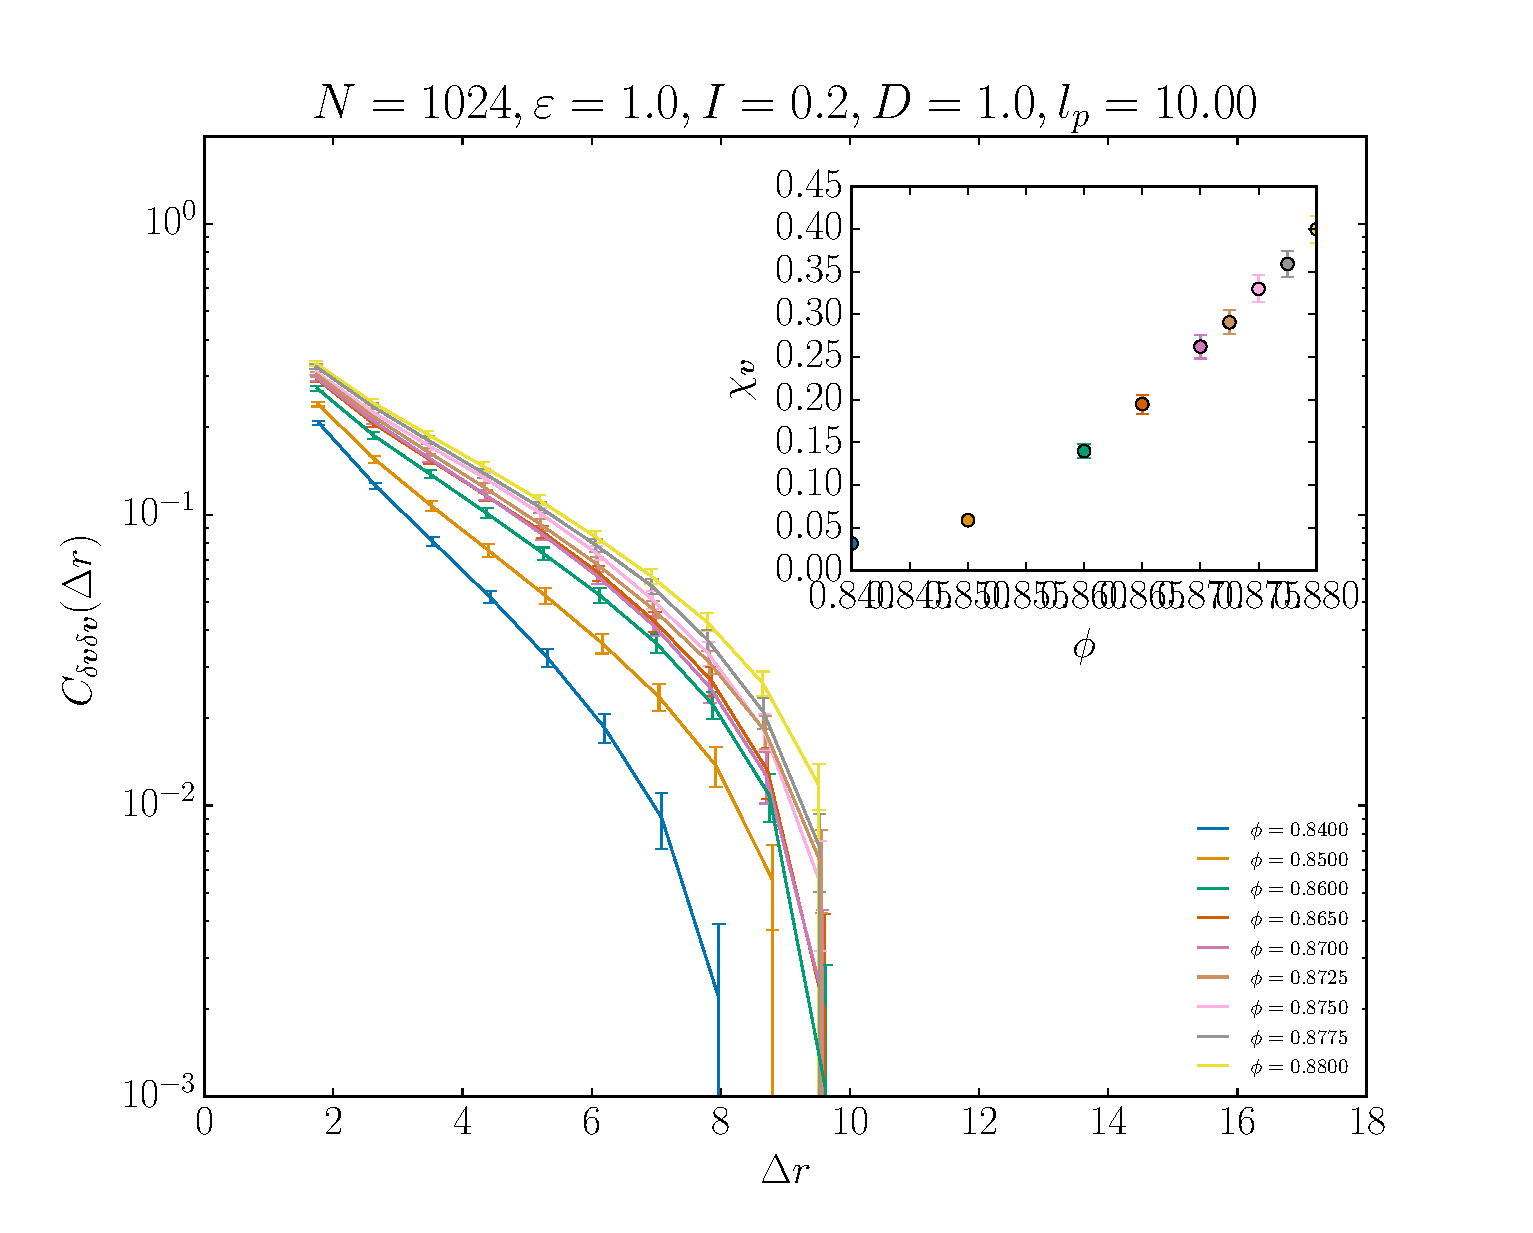
\includegraphics[width=0.35\textwidth]{cvvCMlog_No1024_Tl1000_Rj1000.eps}
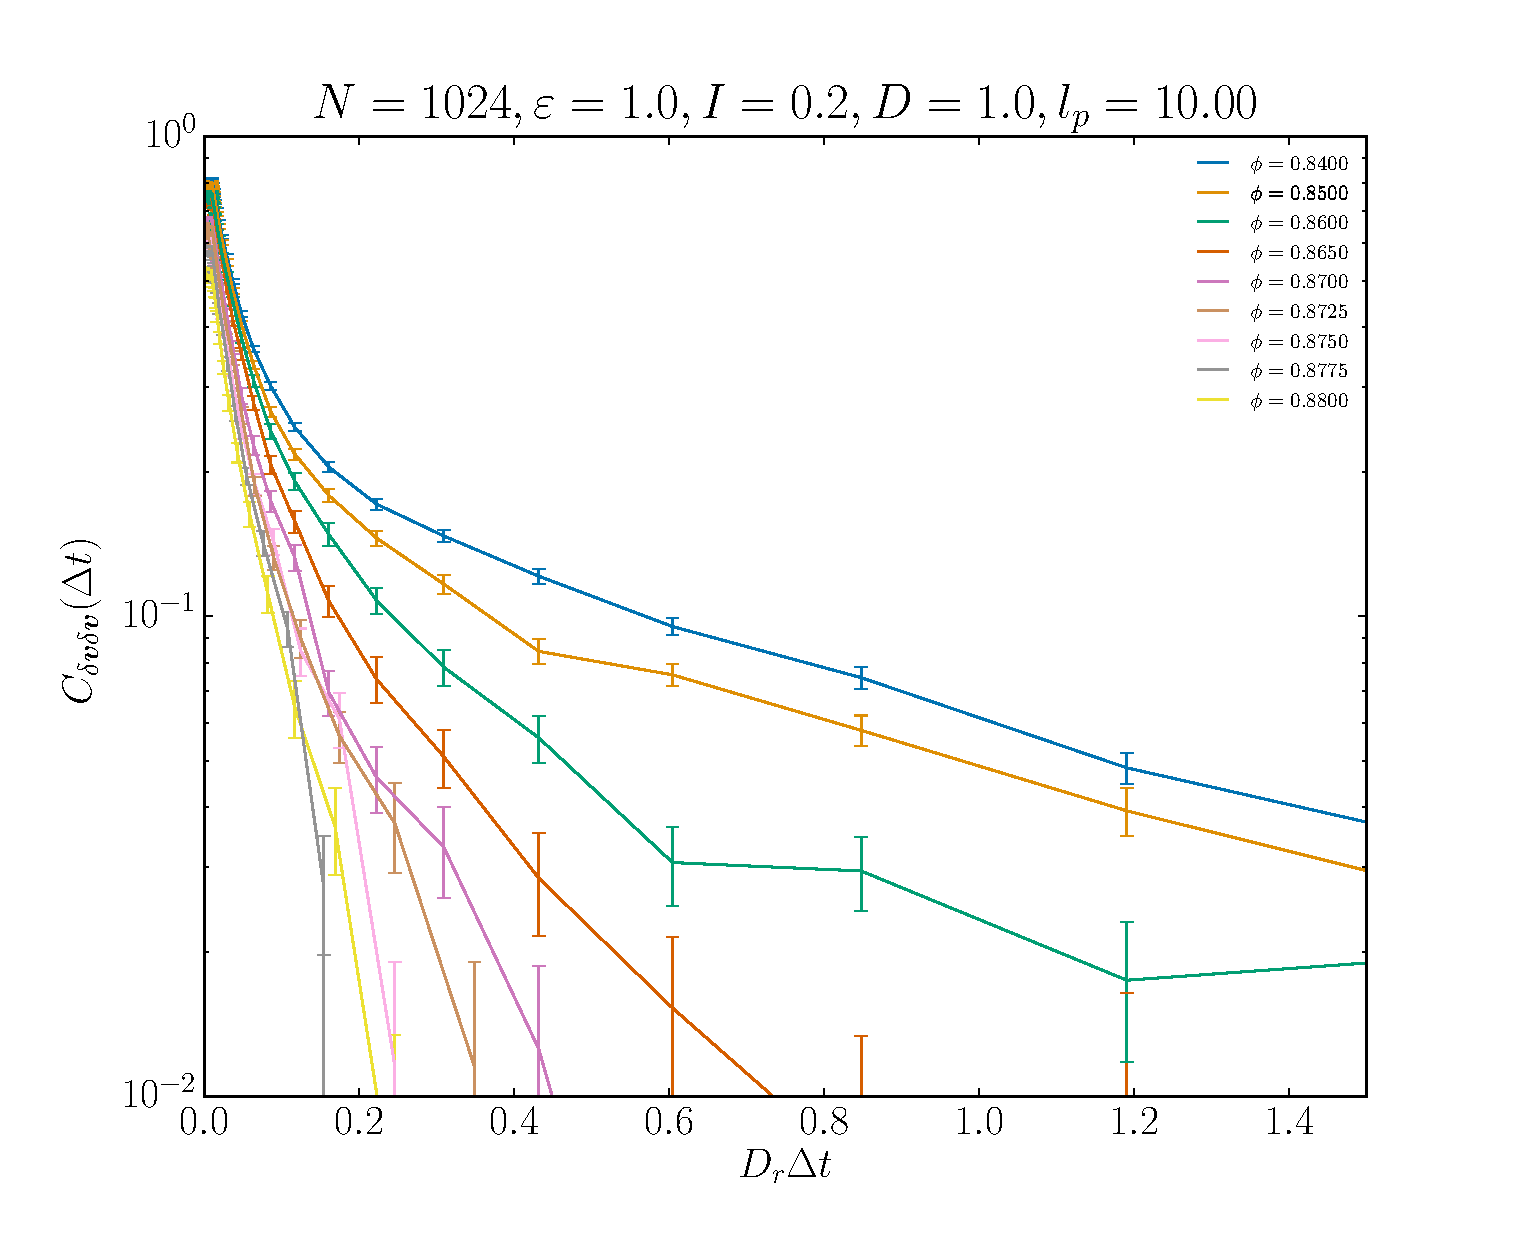
\includegraphics[width=0.35\textwidth]{cvvtCM_No1024_Tl1000_Rj1000.eps}\\
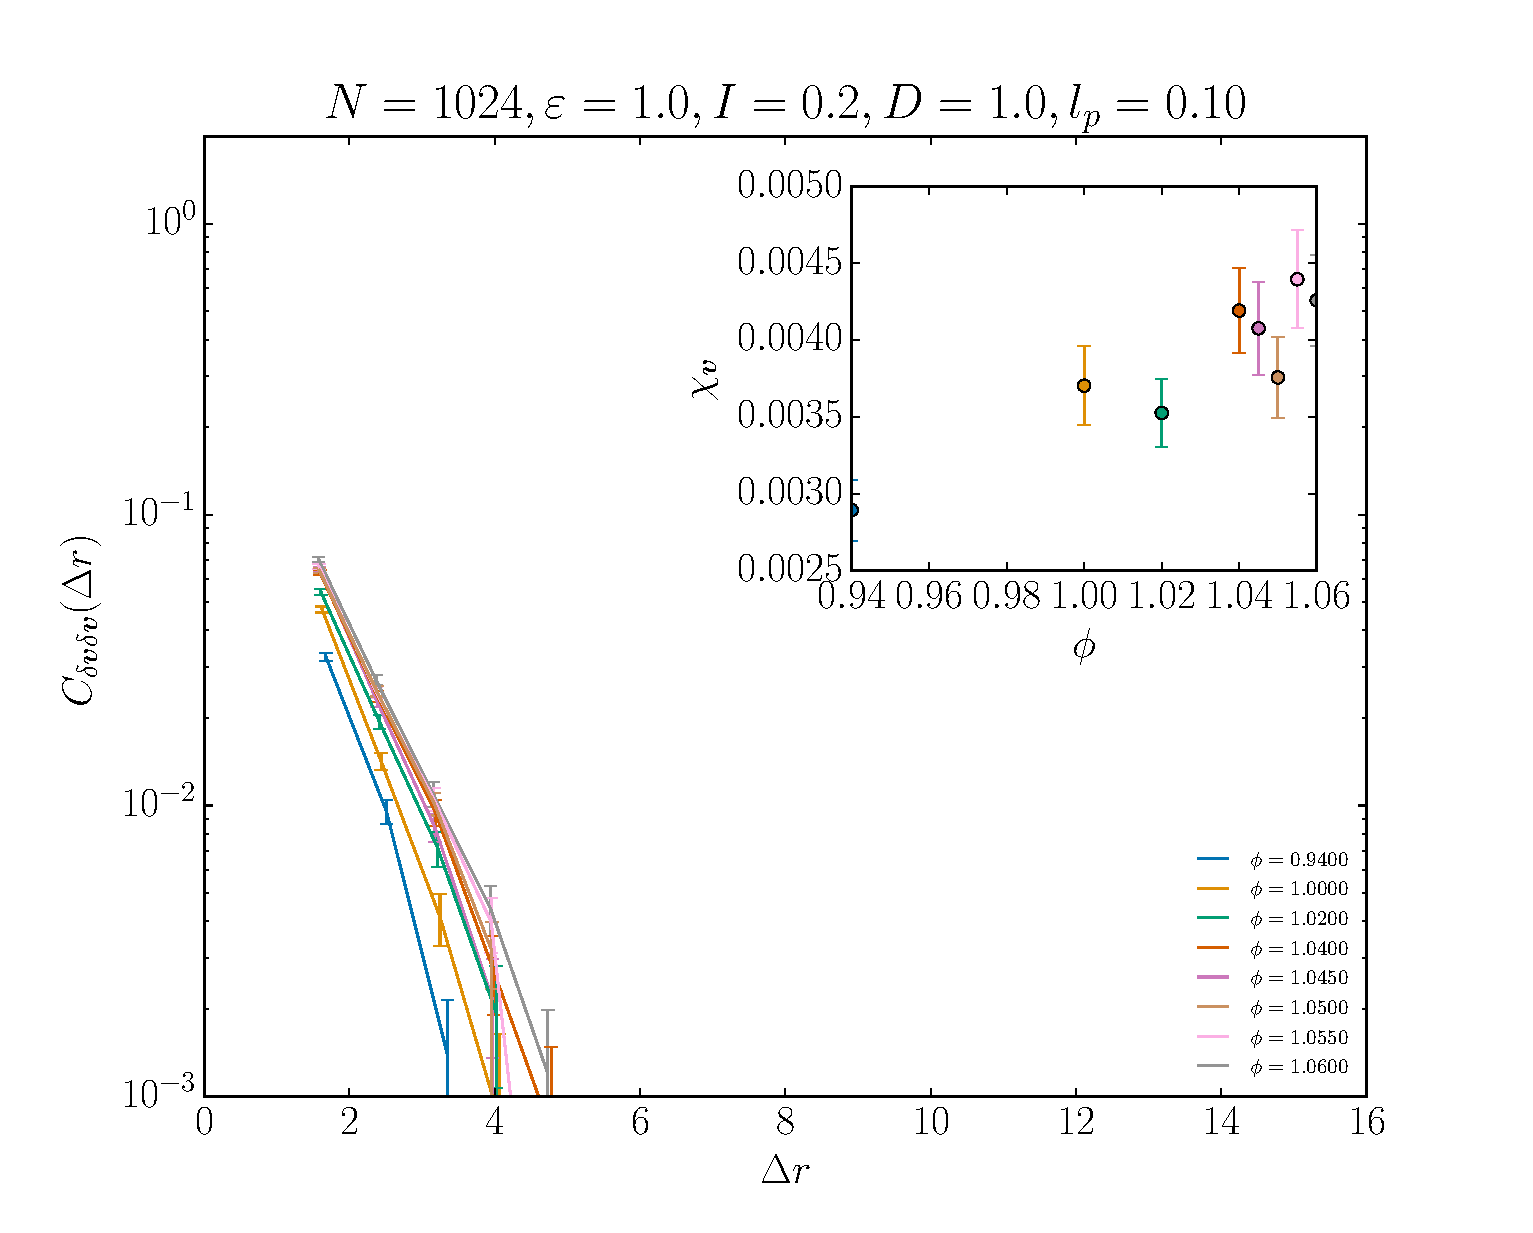
\includegraphics[width=0.35\textwidth]{cvvCMlog_No1024_Tl1000_Rn1000.eps}
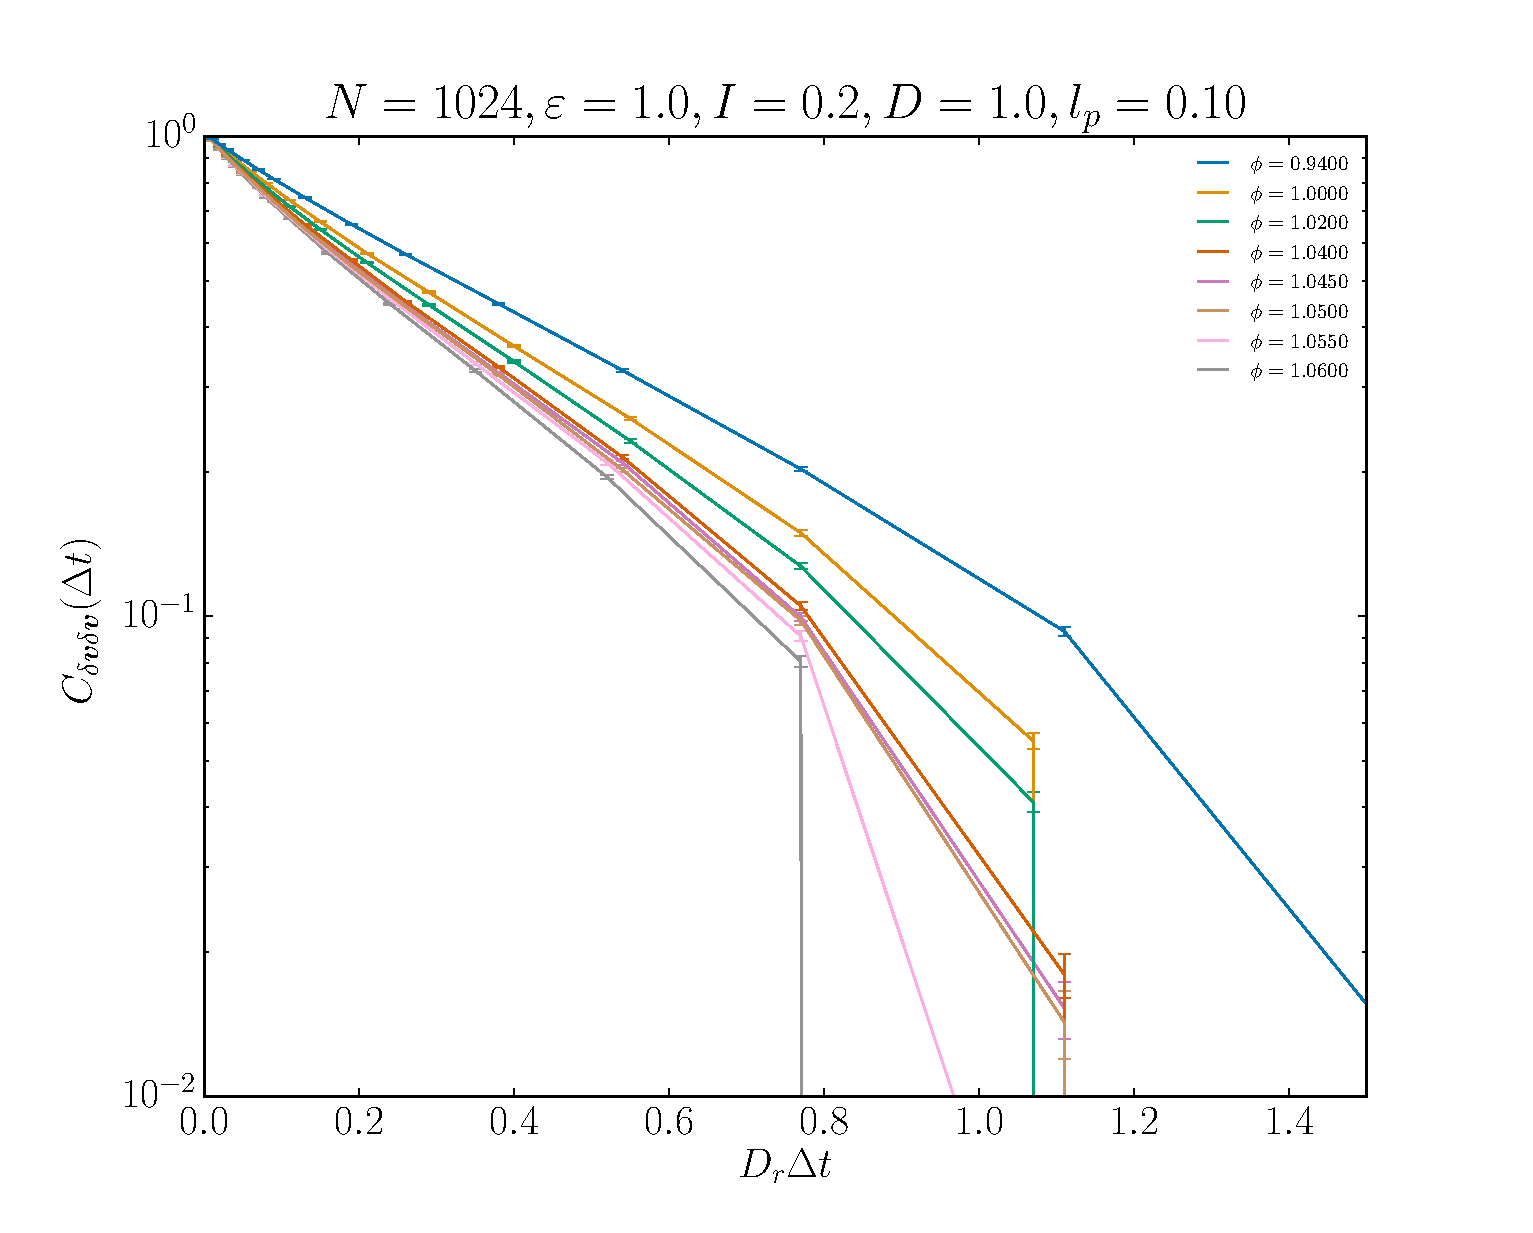
\includegraphics[width=0.35\textwidth]{cvvtCM_No1024_Tl1000_Rn1000.eps}
\caption{Velocity autocorrelation function in {\bf (left)} space {\bf (right)} time at {\bf (top)} $\tau_p = 10^2$ and {\bf (bottom)} $\tau_p = 10^{-2}$.}
\end{figure}

\end{frame}

\begin{frame}{Velocity distribution}

\begin{figure}
\centering
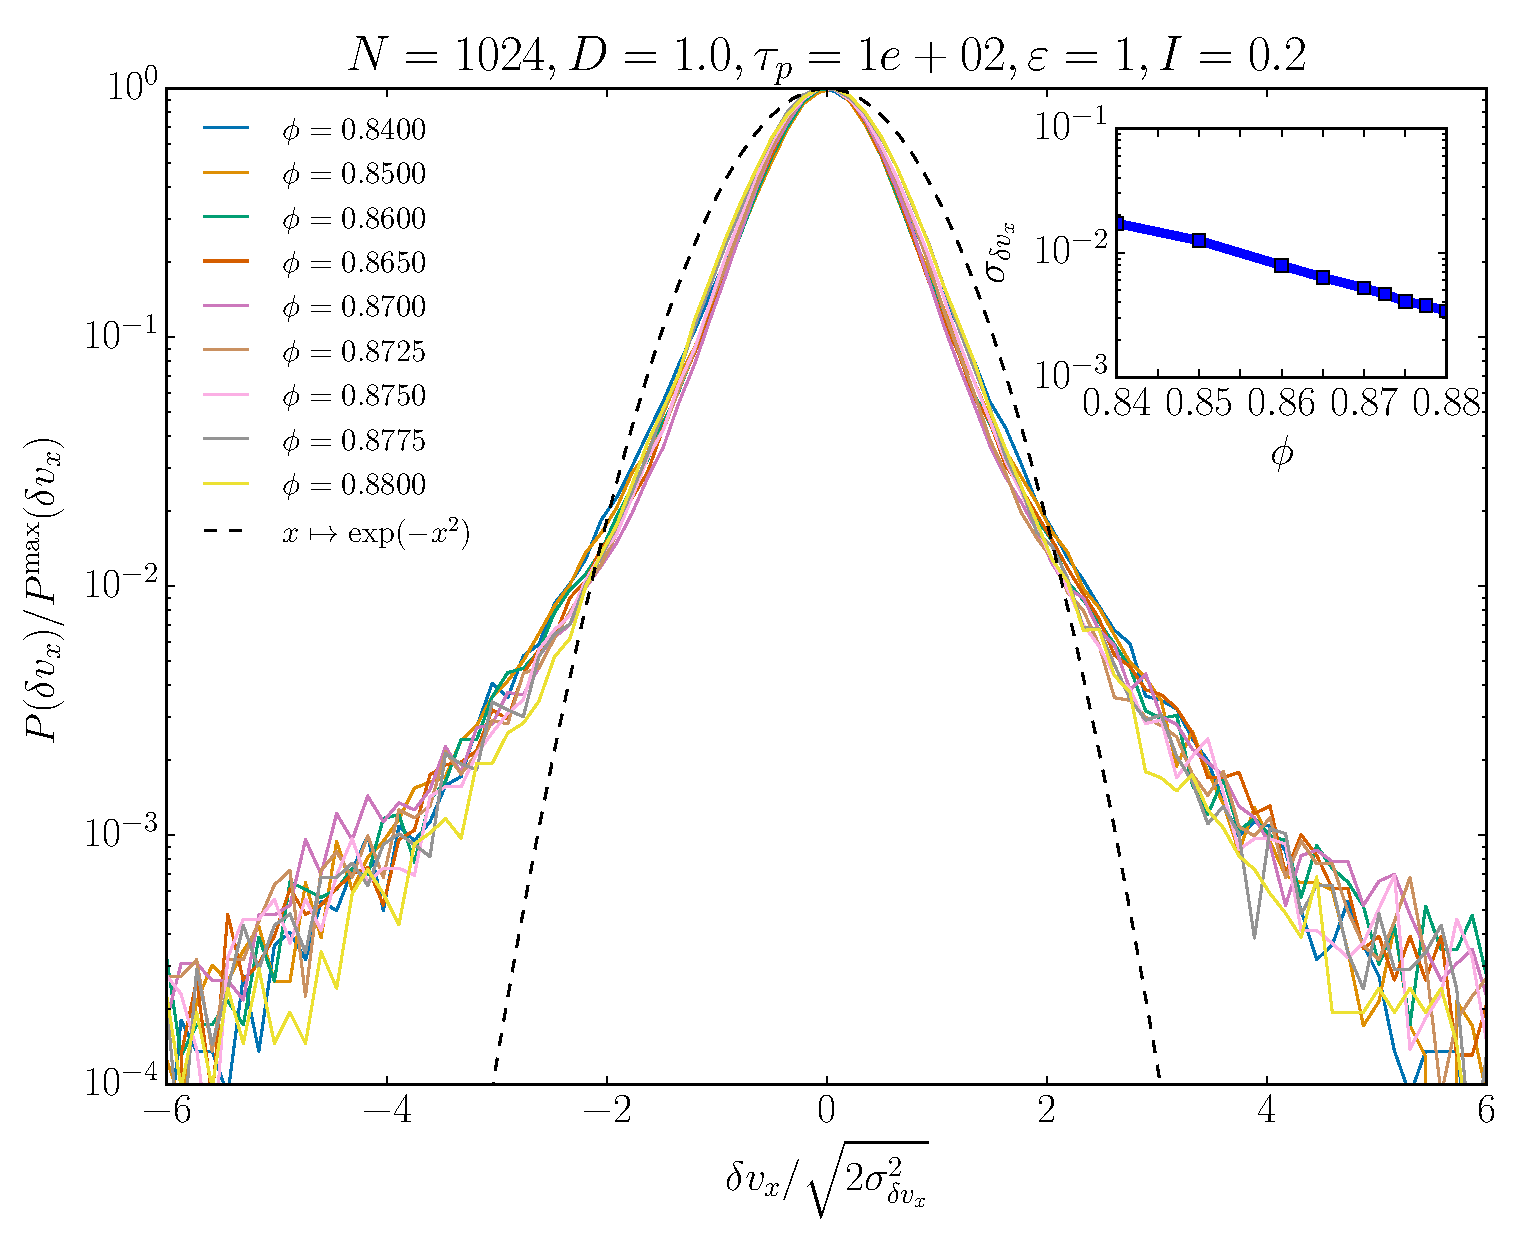
\includegraphics[width=0.35\textwidth]{No1024_Fl1000_Vl0000_Tl1000_Rj1000.pvx.eps}
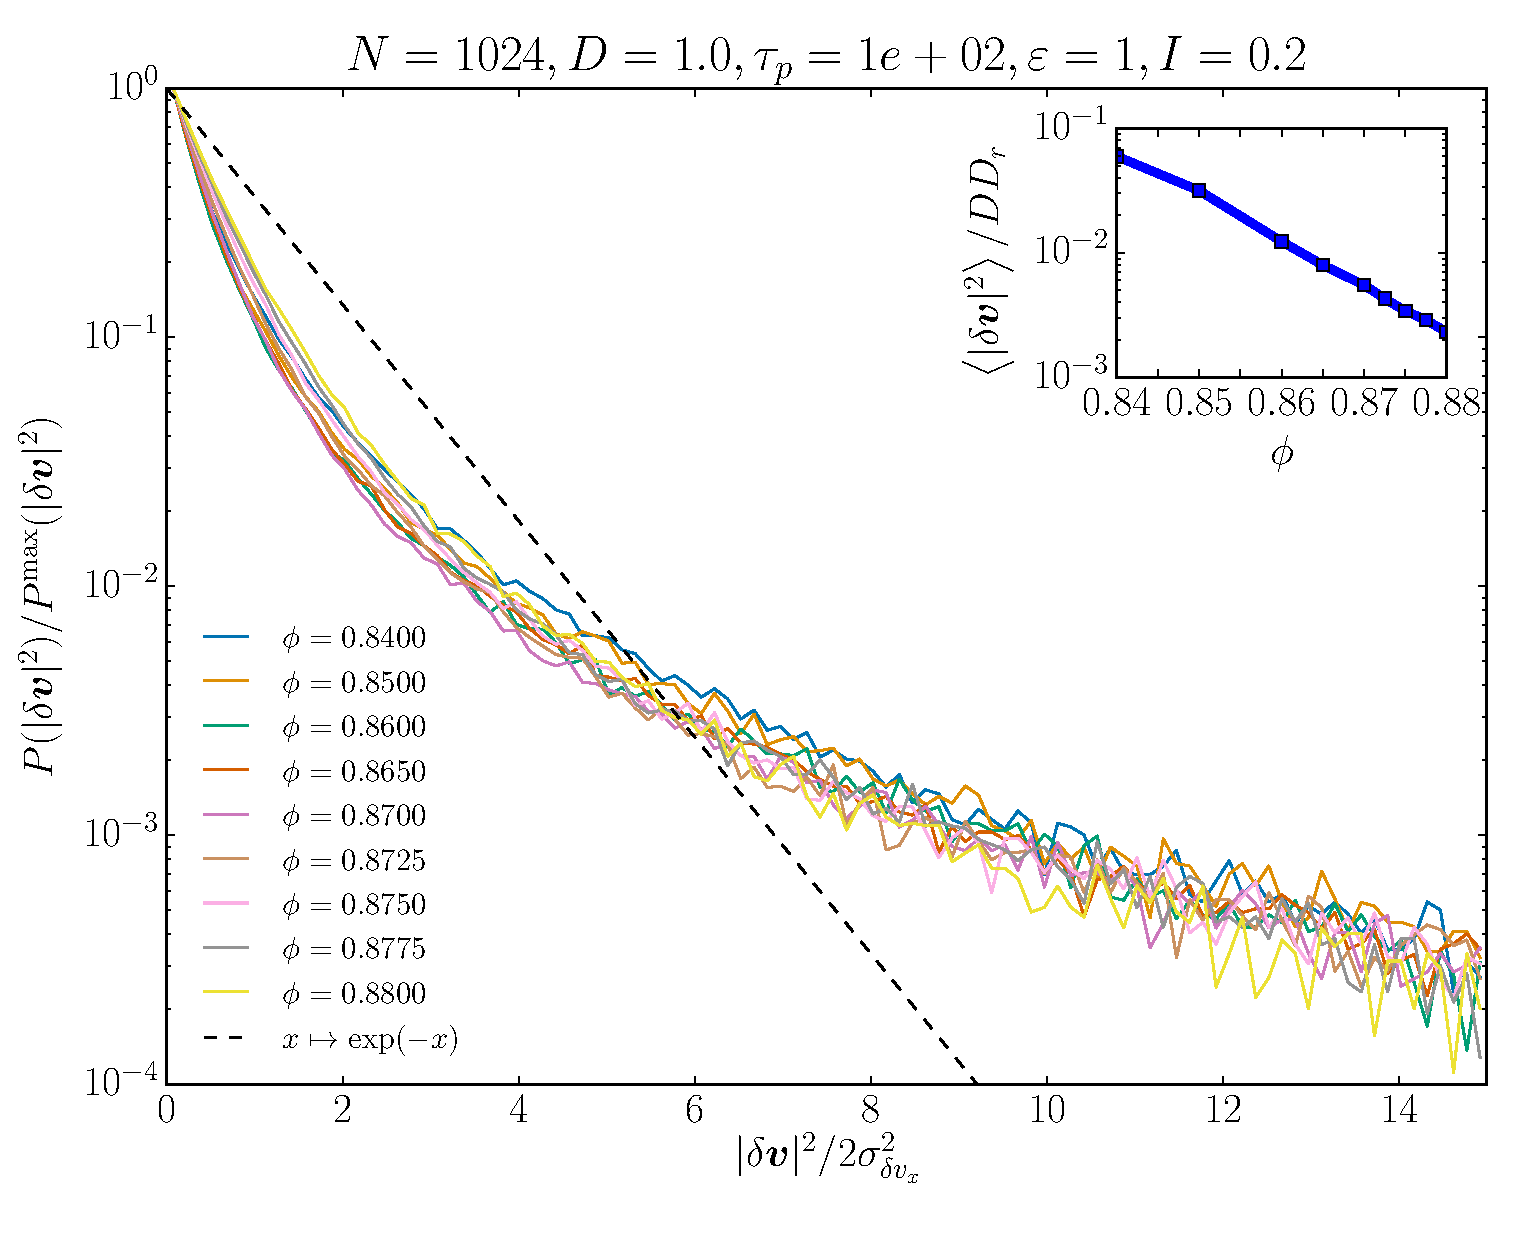
\includegraphics[width=0.35\textwidth]{No1024_Fl1000_Vl0000_Tl1000_Rj1000.pv2.eps}\\
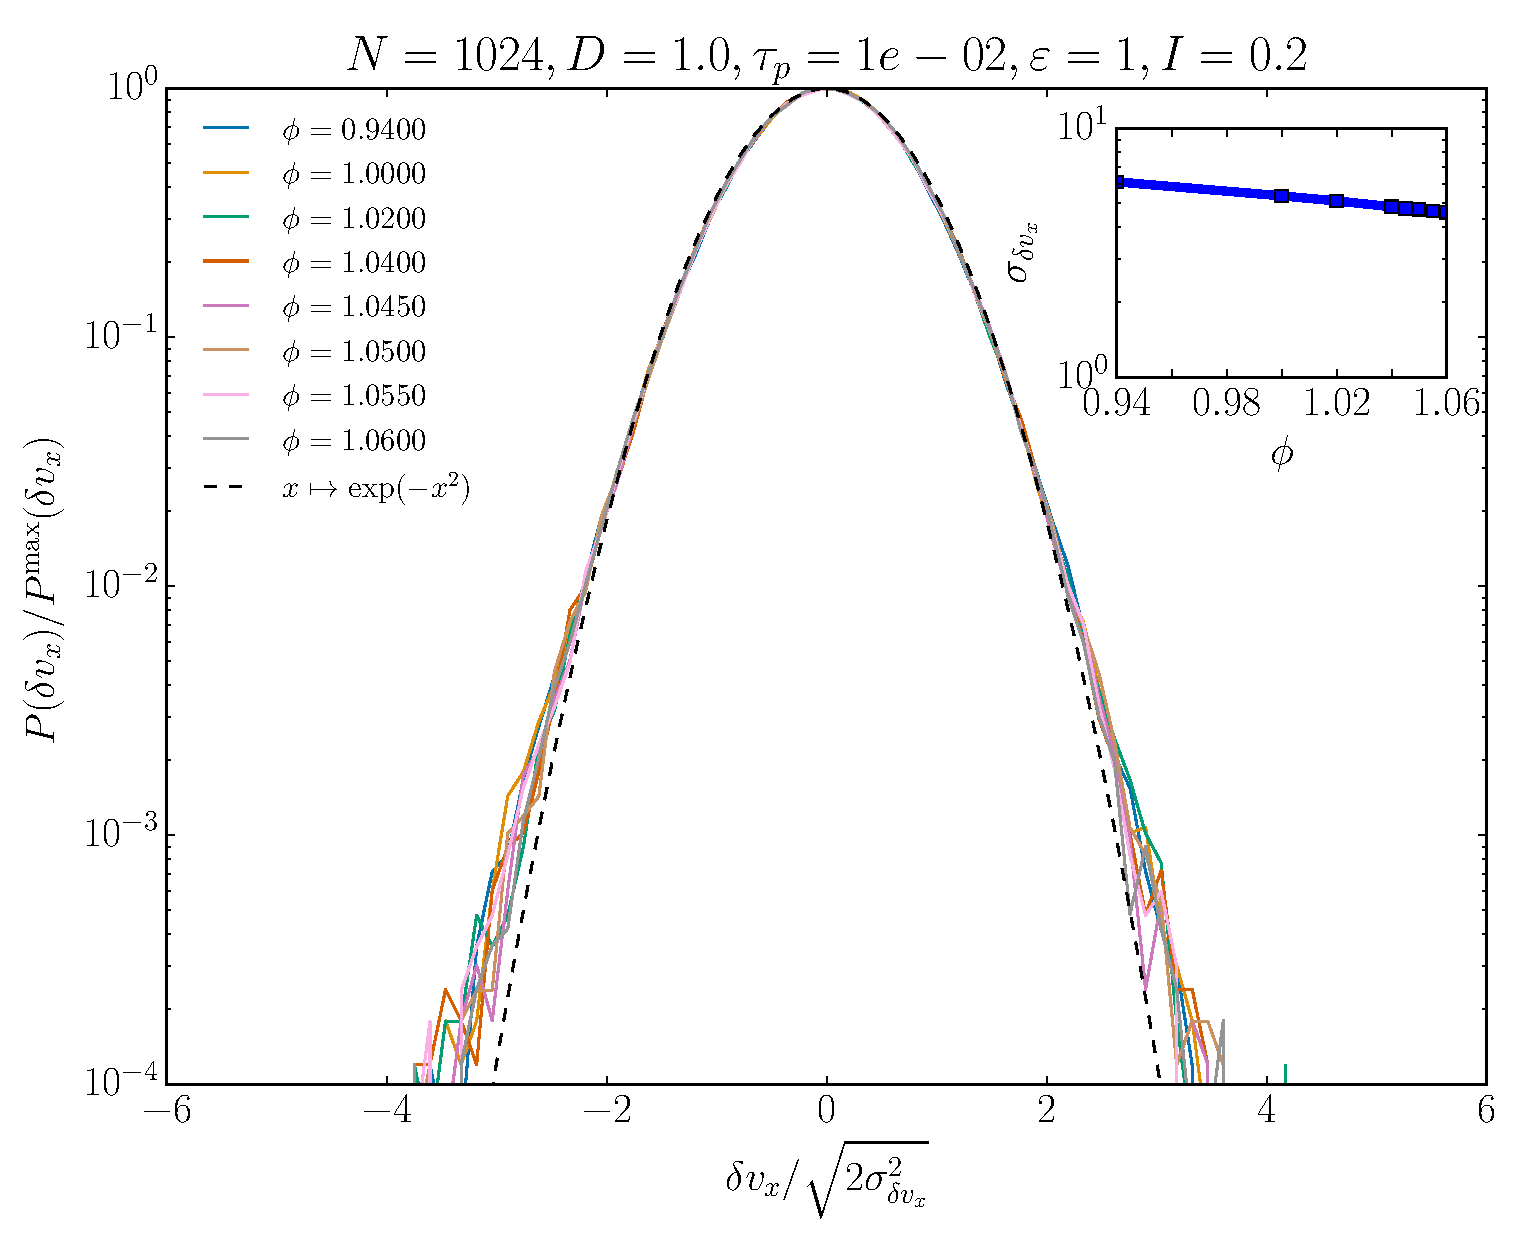
\includegraphics[width=0.35\textwidth]{No1024_Fl1000_Vl0000_Tl1000_Rn1000.pvx.eps}
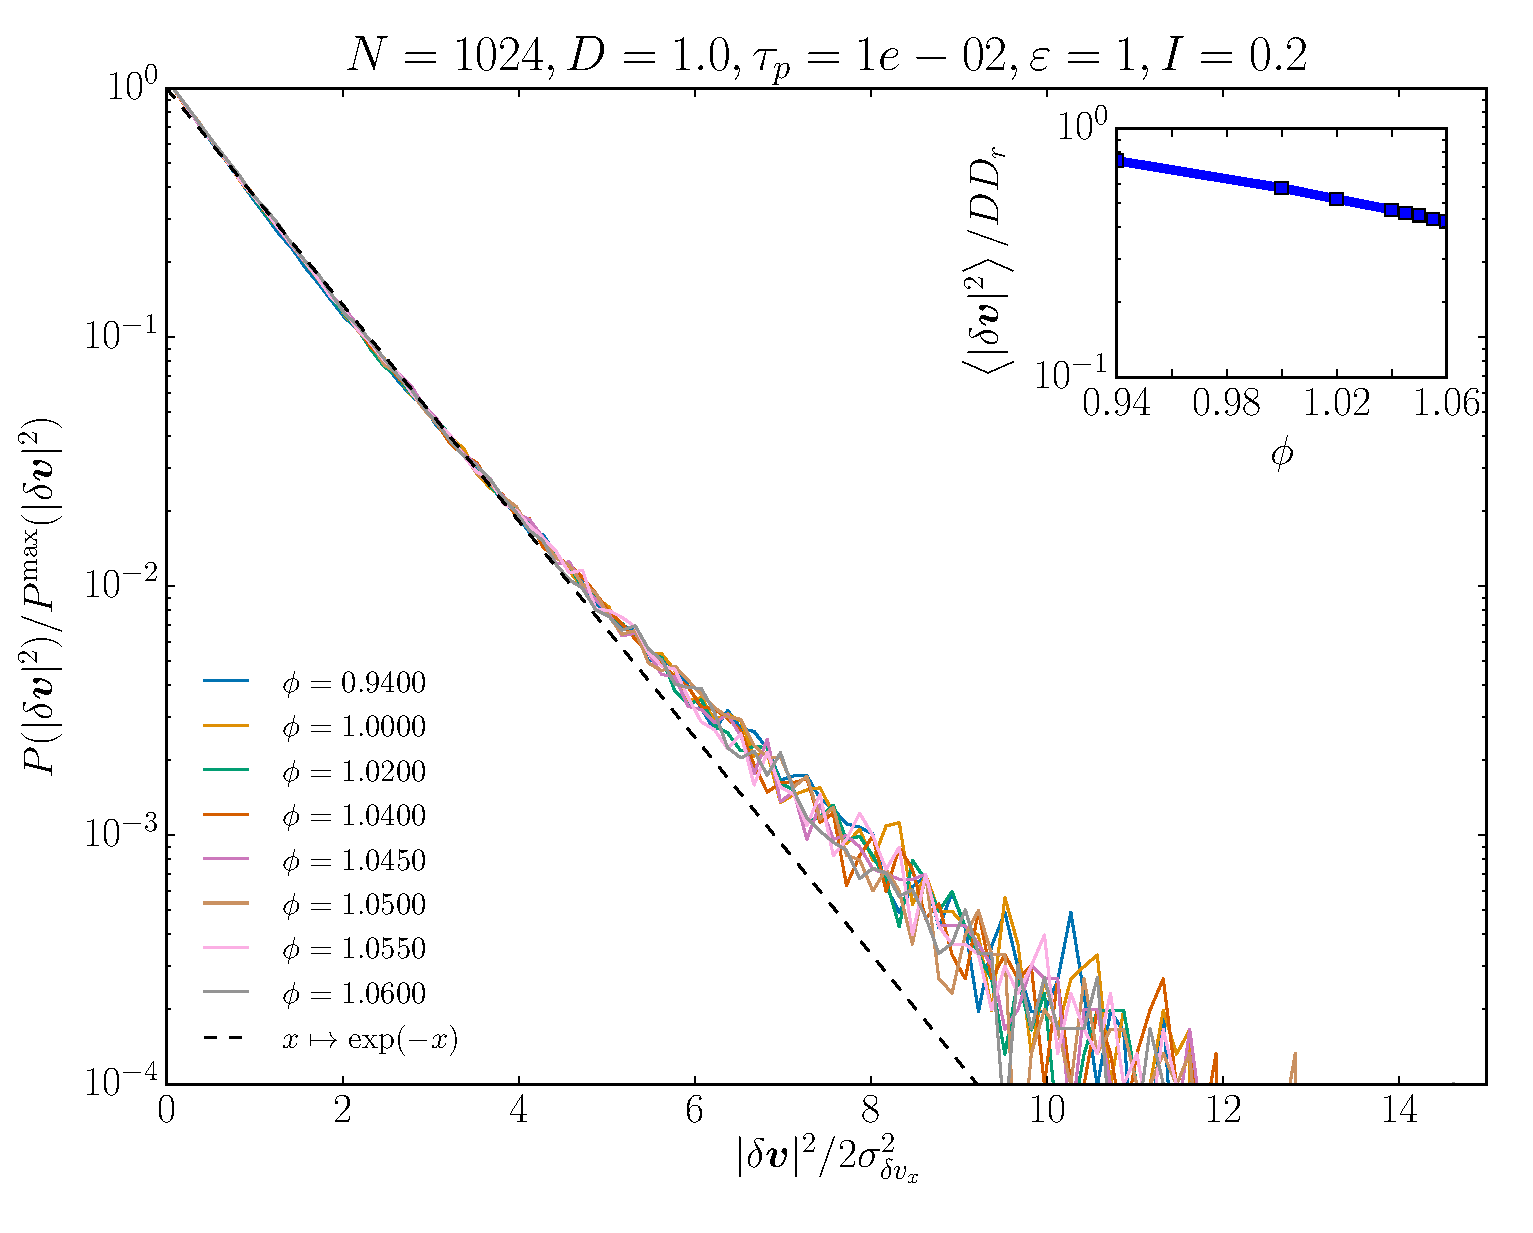
\includegraphics[width=0.35\textwidth]{No1024_Fl1000_Vl0000_Tl1000_Rn1000.pv2.eps}
\caption{Distributions of {\bf (left)} $\boldsymbol{v}\cdot\boldsymbol{e}_x$ and {\bf (right)} $|\boldsymbol{v}|^2$ at {\bf (top)} $\tau_p = 10^2$ and {\bf (bottom)} $\tau_p = 10^{-2}$.}
\end{figure}

\vspace{-10pt}
\footfullcitenomark{caprini2020active}

\end{frame}

\begin{frame}{Time series of kinetic energy}

\begin{figure}
\centering
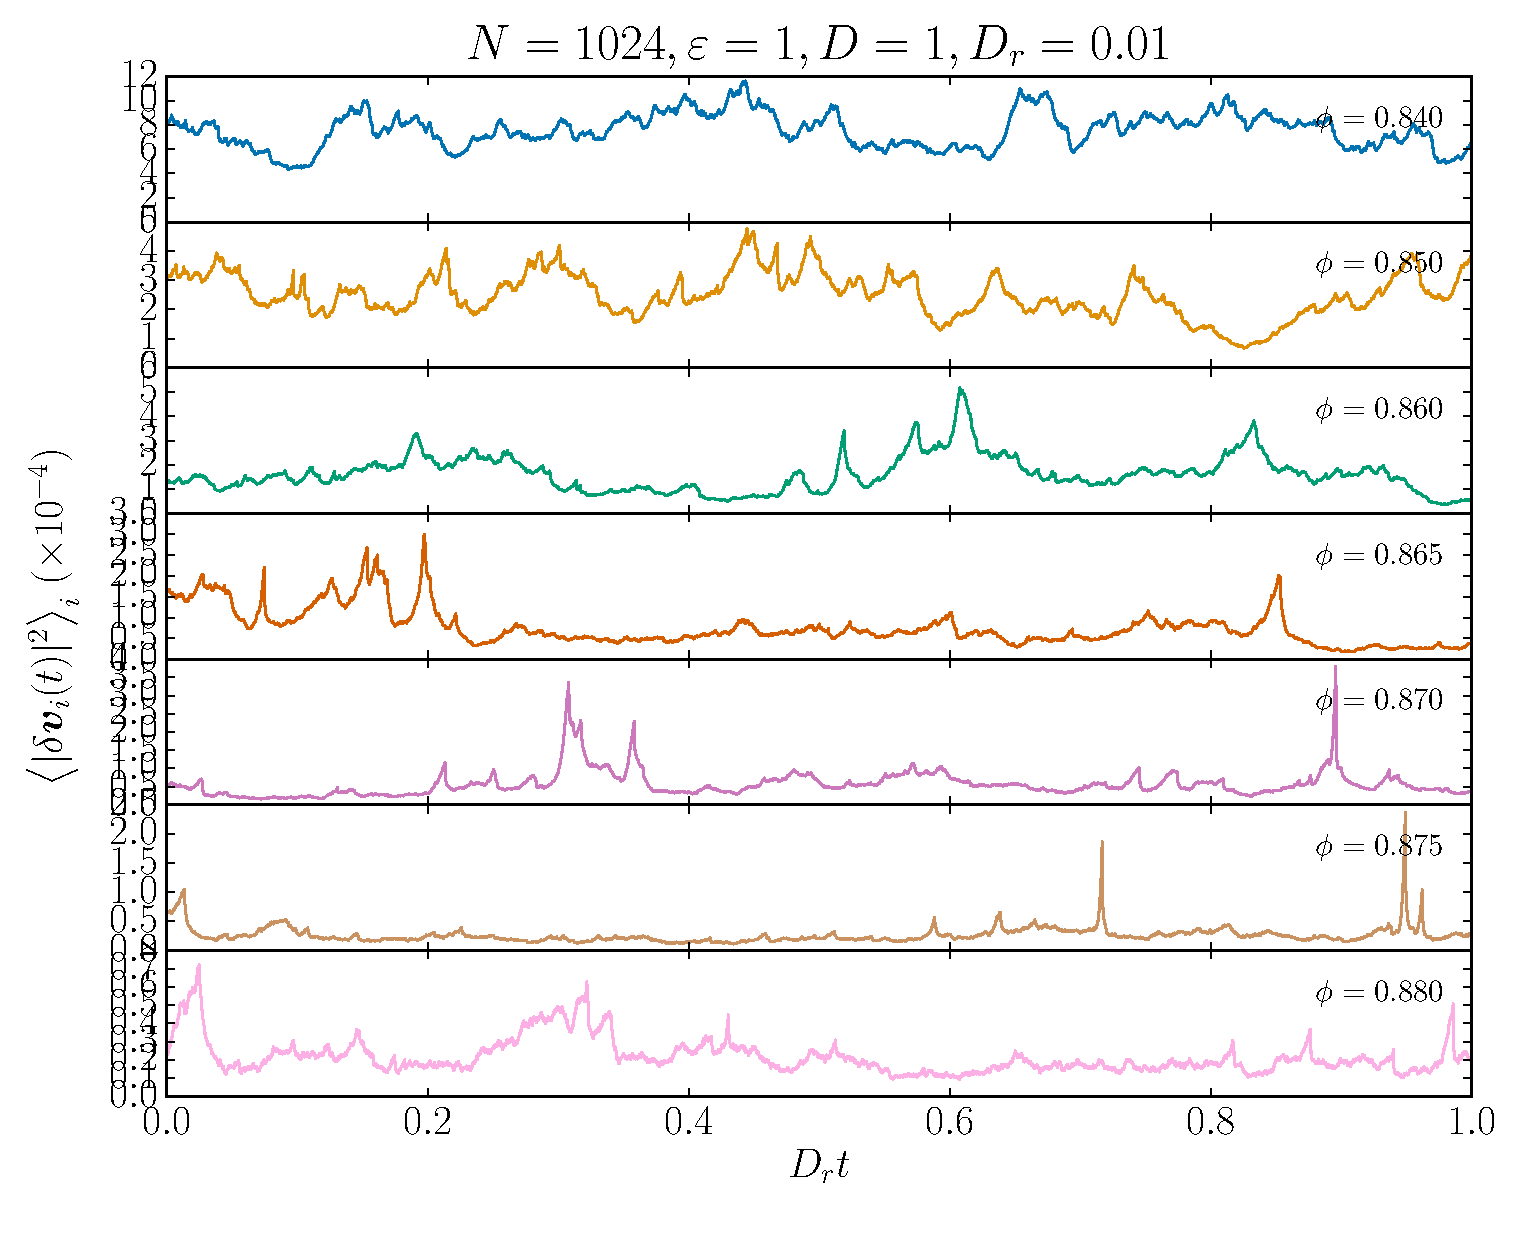
\includegraphics[width=0.45\textwidth]{No1024_Fl1000_Vl0000_Tl1000_Rj1000.ecC.eps}
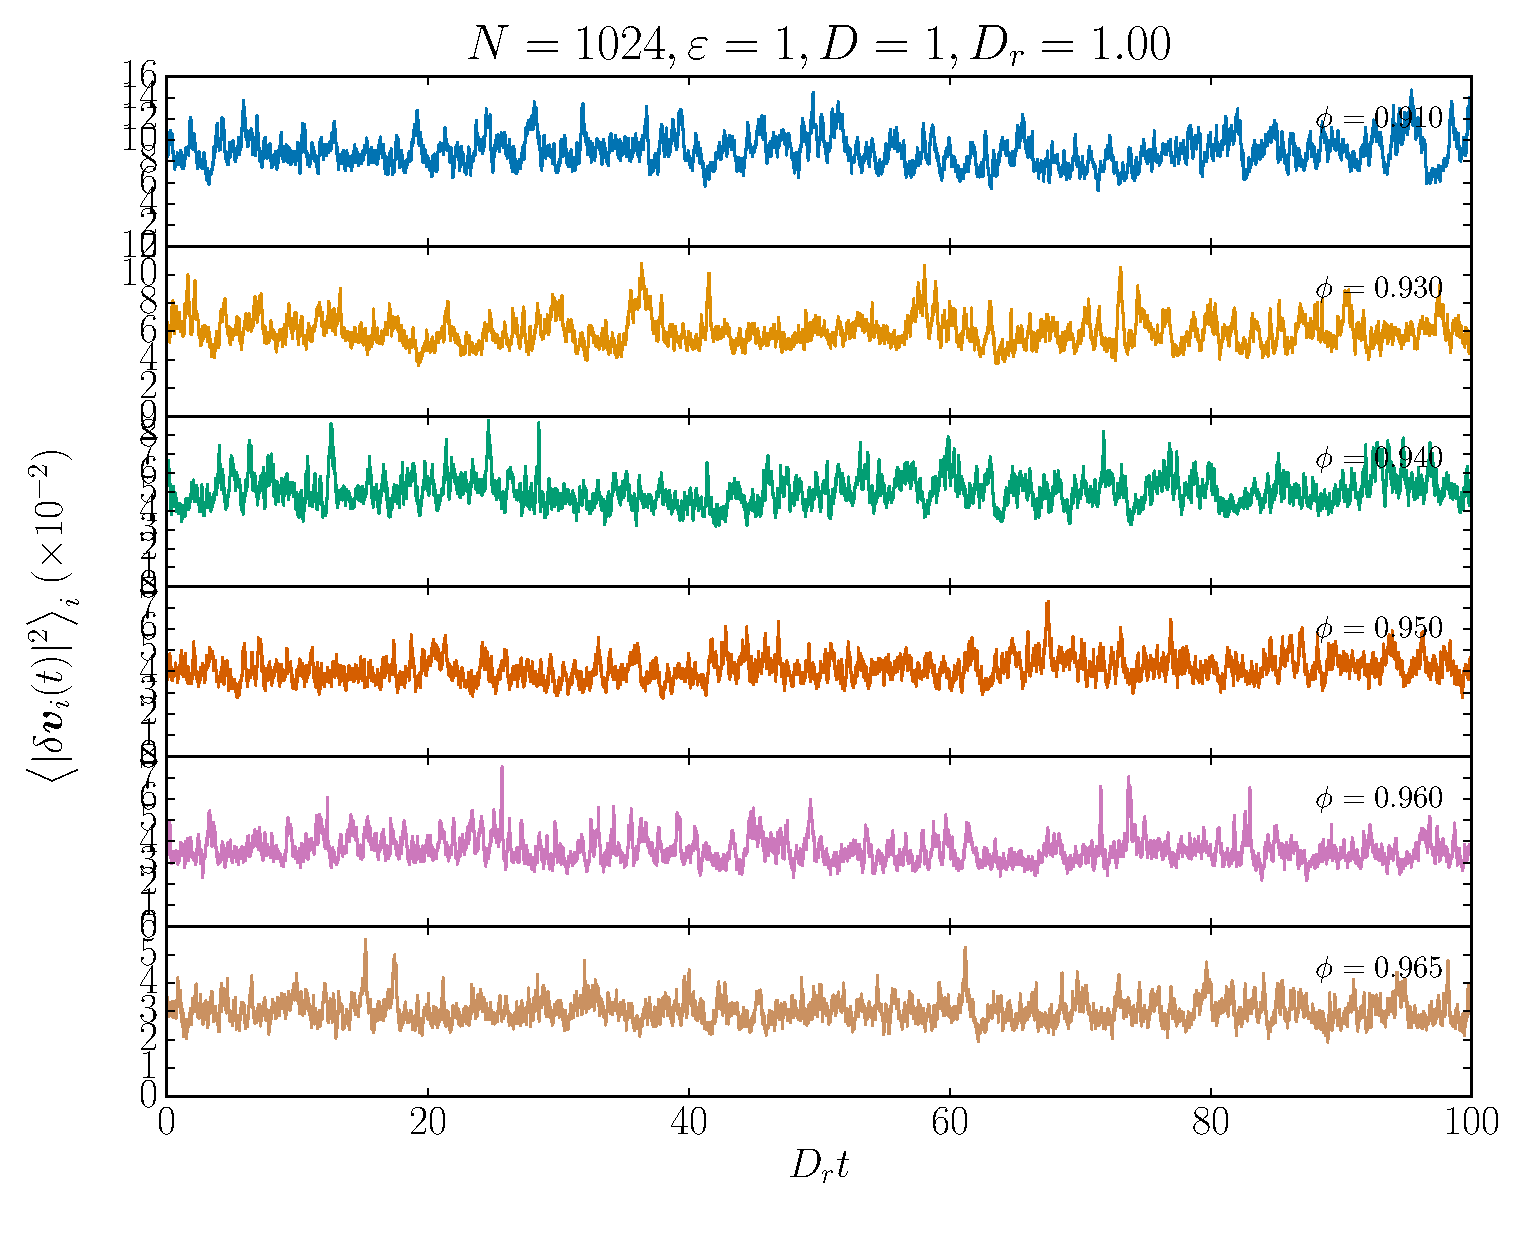
\includegraphics[width=0.45\textwidth]{No1024_Fl1000_Vl0000_Tl1000_Rl1000.ecC.eps}
\caption{Time series of kinetic energy at {\bf (top)} $\tau_p = 10^2$ and {\bf (bottom)} $\tau_p = 10^0$.}
\end{figure}

\footfullcitenomark{mandal2020extreme}
\footfullcitenomark{caprini2020active}

\end{frame}

\begin{frame}{Swim velocity}

\begin{equation}
v(\rho)/\left<|\boldsymbol{p}_i|\right> = 1 + \left<-\nabla_i U \cdot \boldsymbol{p}_i/|\boldsymbol{p}_i|\right>
\end{equation}

\begin{figure}
\centering
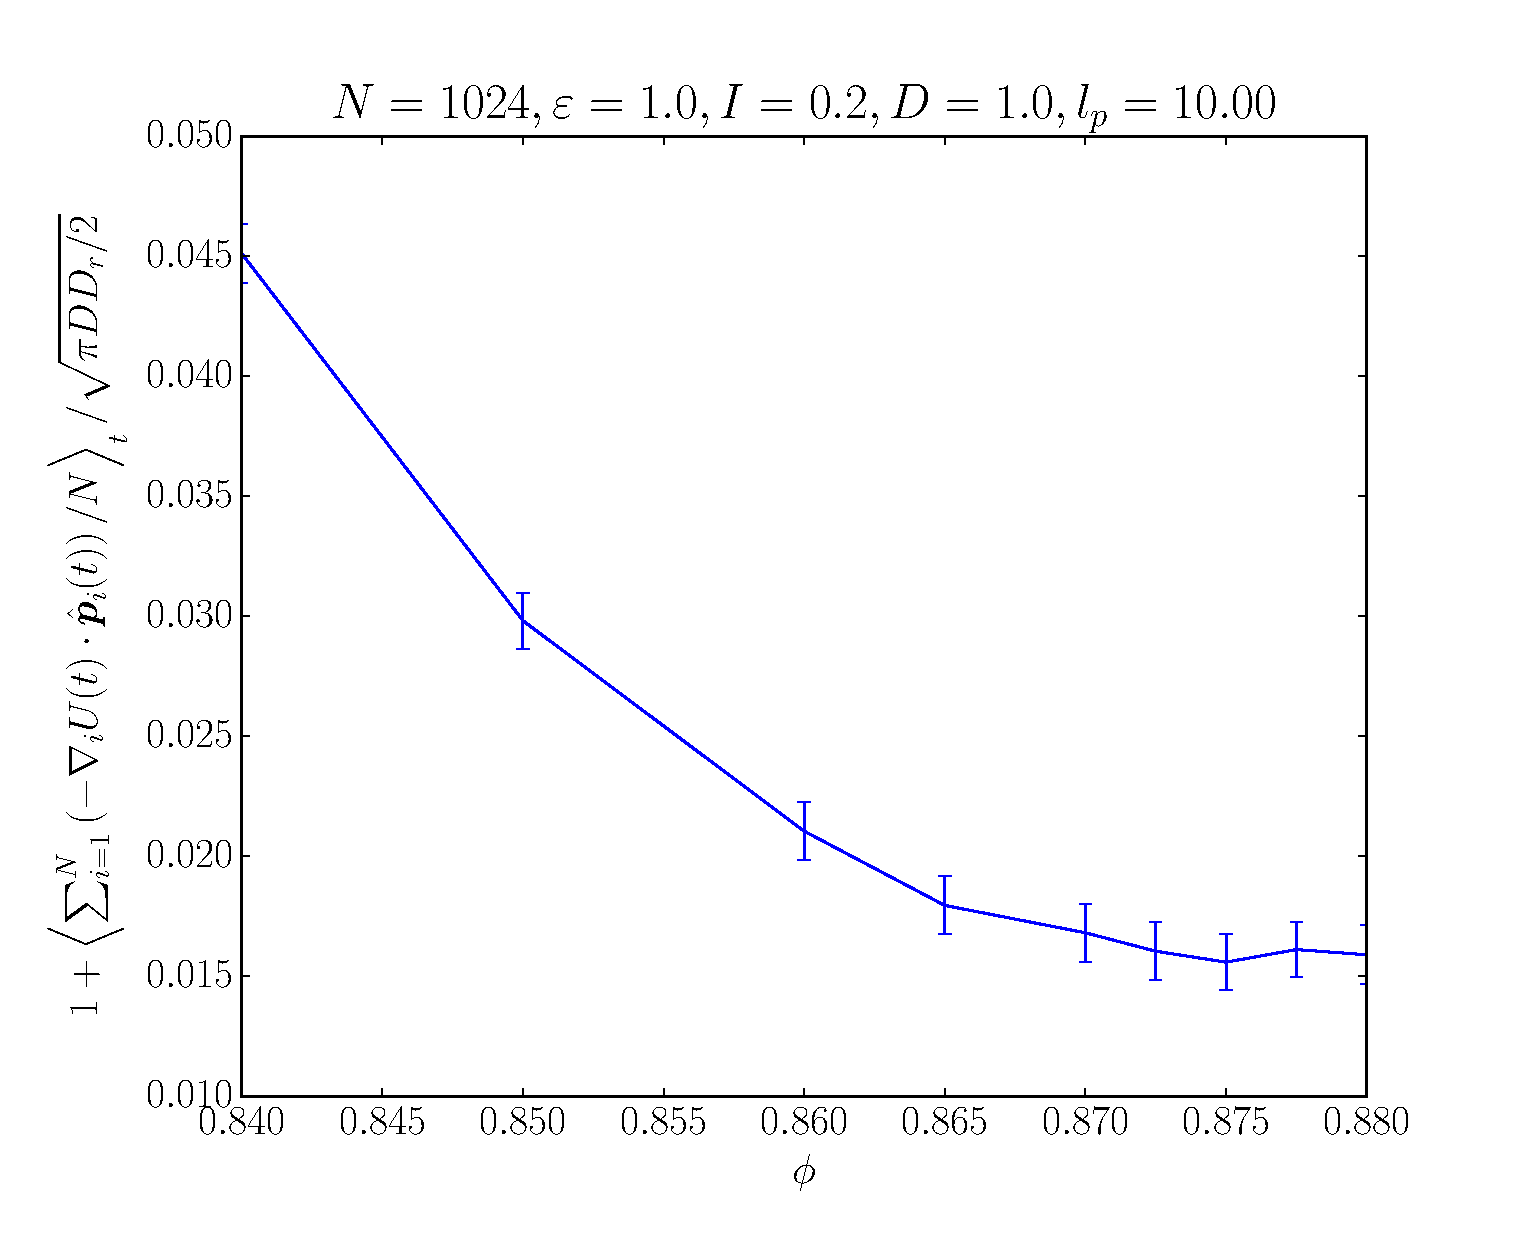
\includegraphics[width=0.30\textwidth]{fo_No1024_Tl1000_Rj1000.eps}
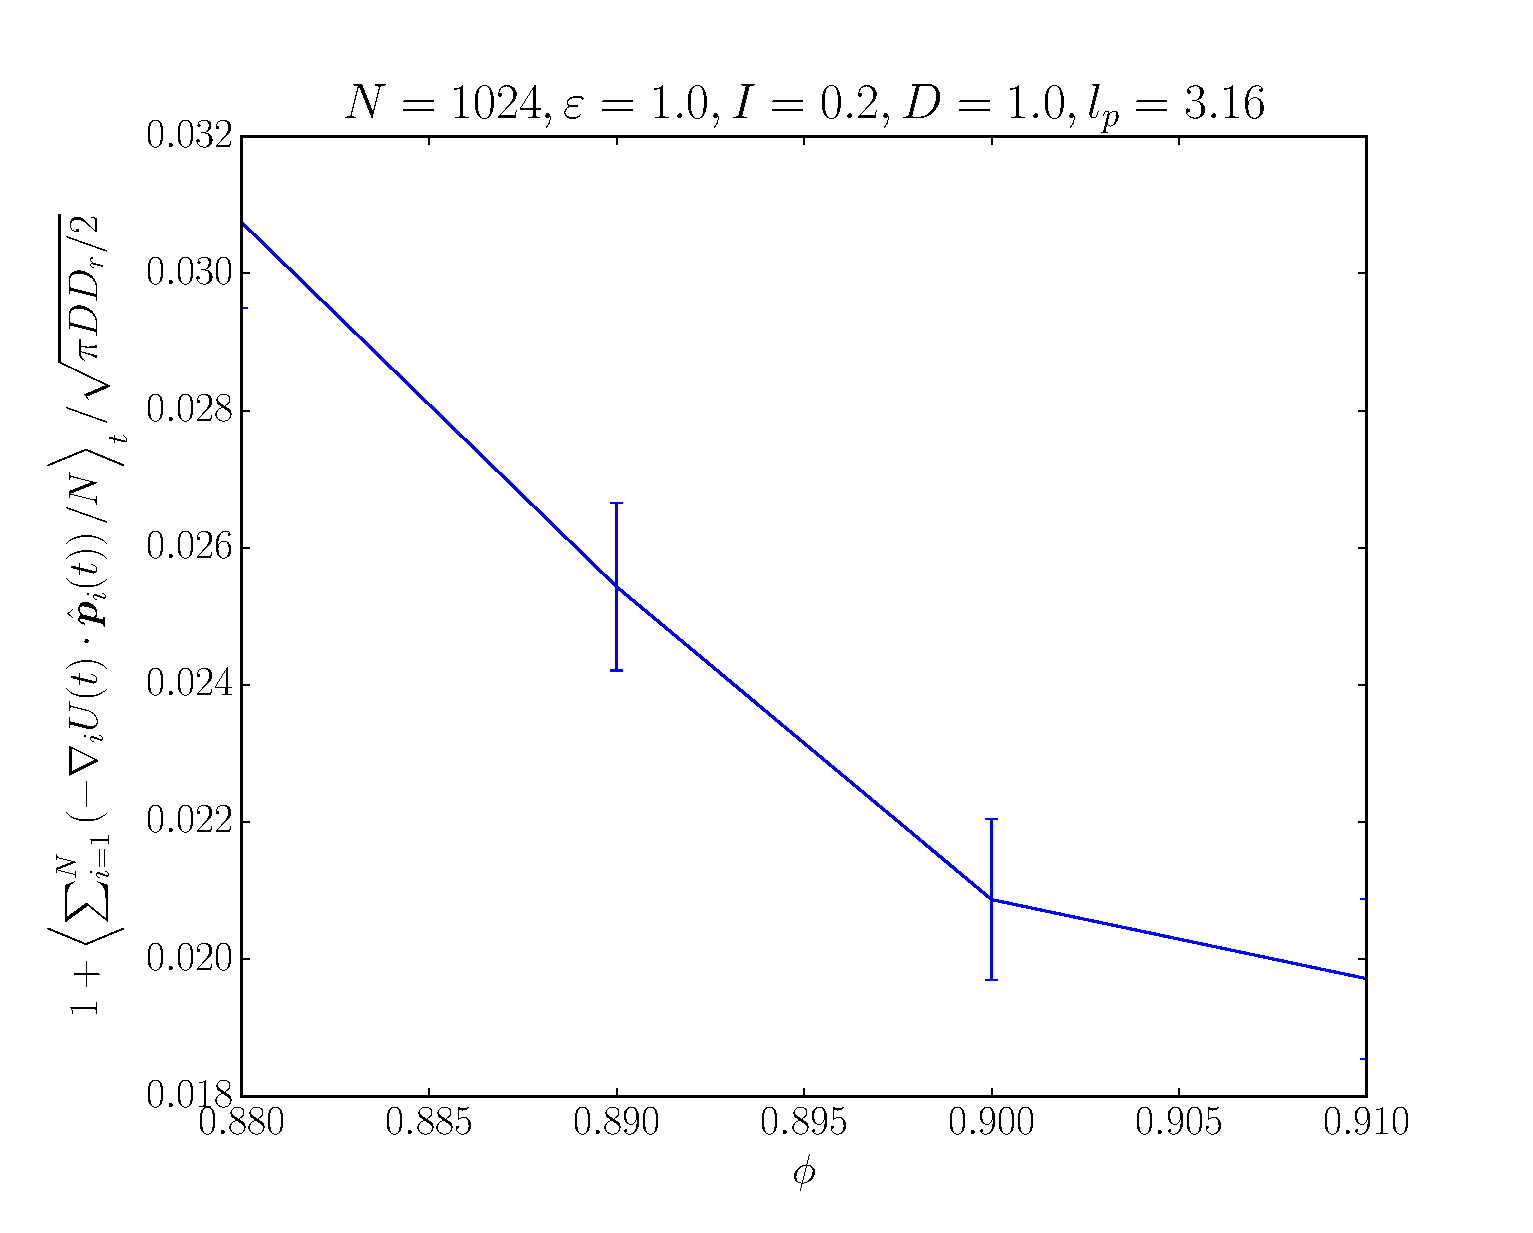
\includegraphics[width=0.30\textwidth]{fo_No1024_Tl1000_Rk1000.eps}\\
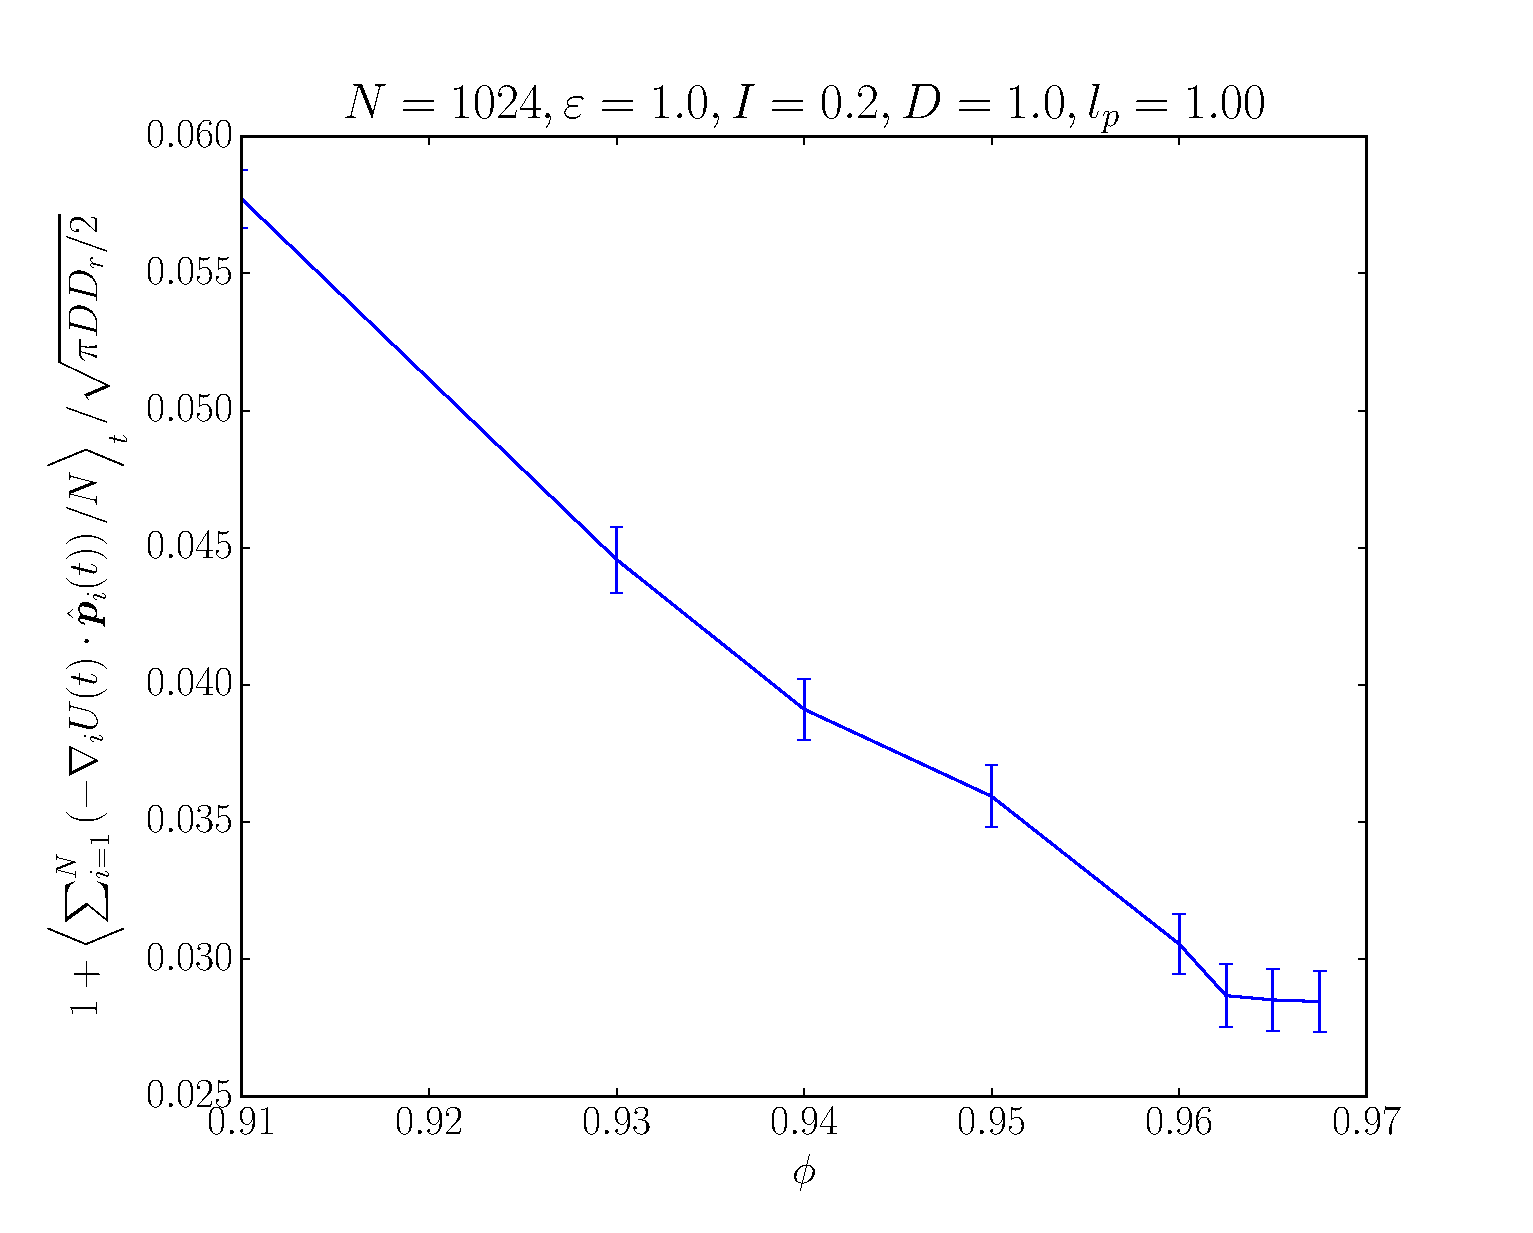
\includegraphics[width=0.30\textwidth]{fo_No1024_Tl1000_Rl1000.eps}
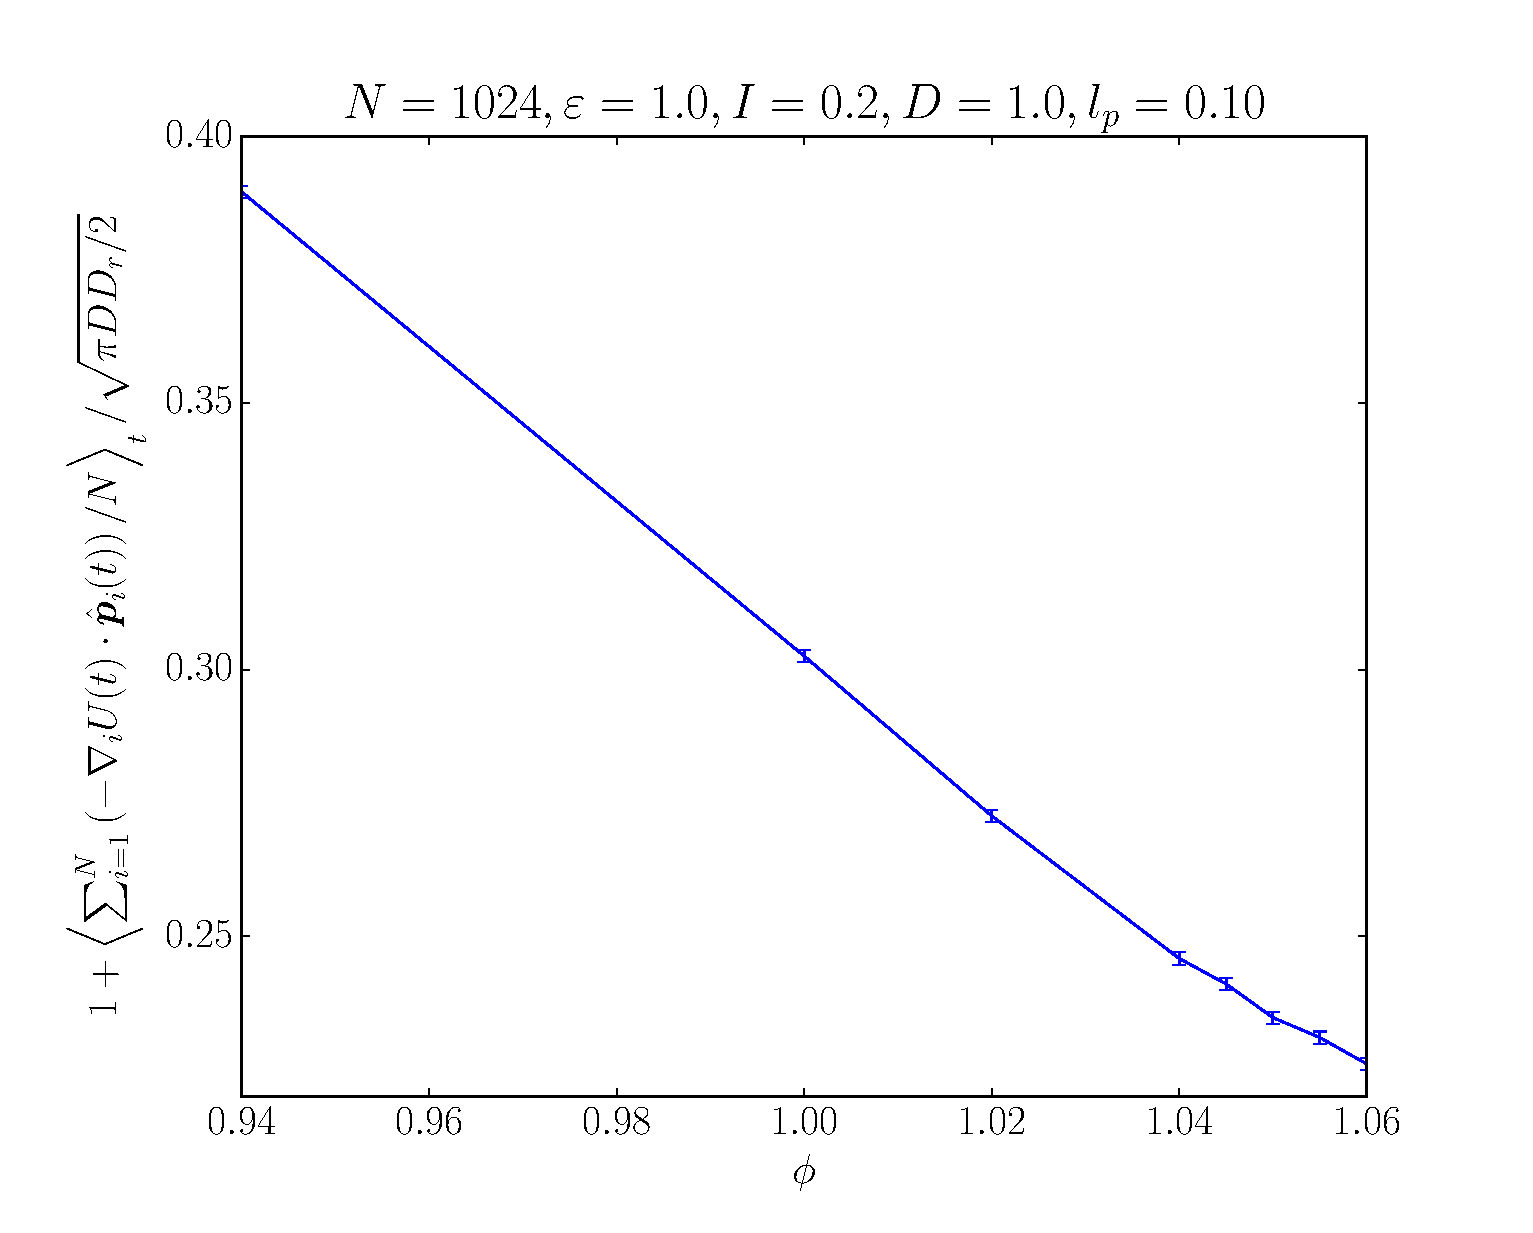
\includegraphics[width=0.30\textwidth]{fo_No1024_Tl1000_Rn1000.eps}
\caption{Rescaled swim velocity.}
\end{figure}

\vspace{-10pt}
\footfullcitenomark{solon2015pressure}

\end{frame}

\section{Outlook}

\begin{frame}{Tentative phase diagram}

\begin{figure}
\centering
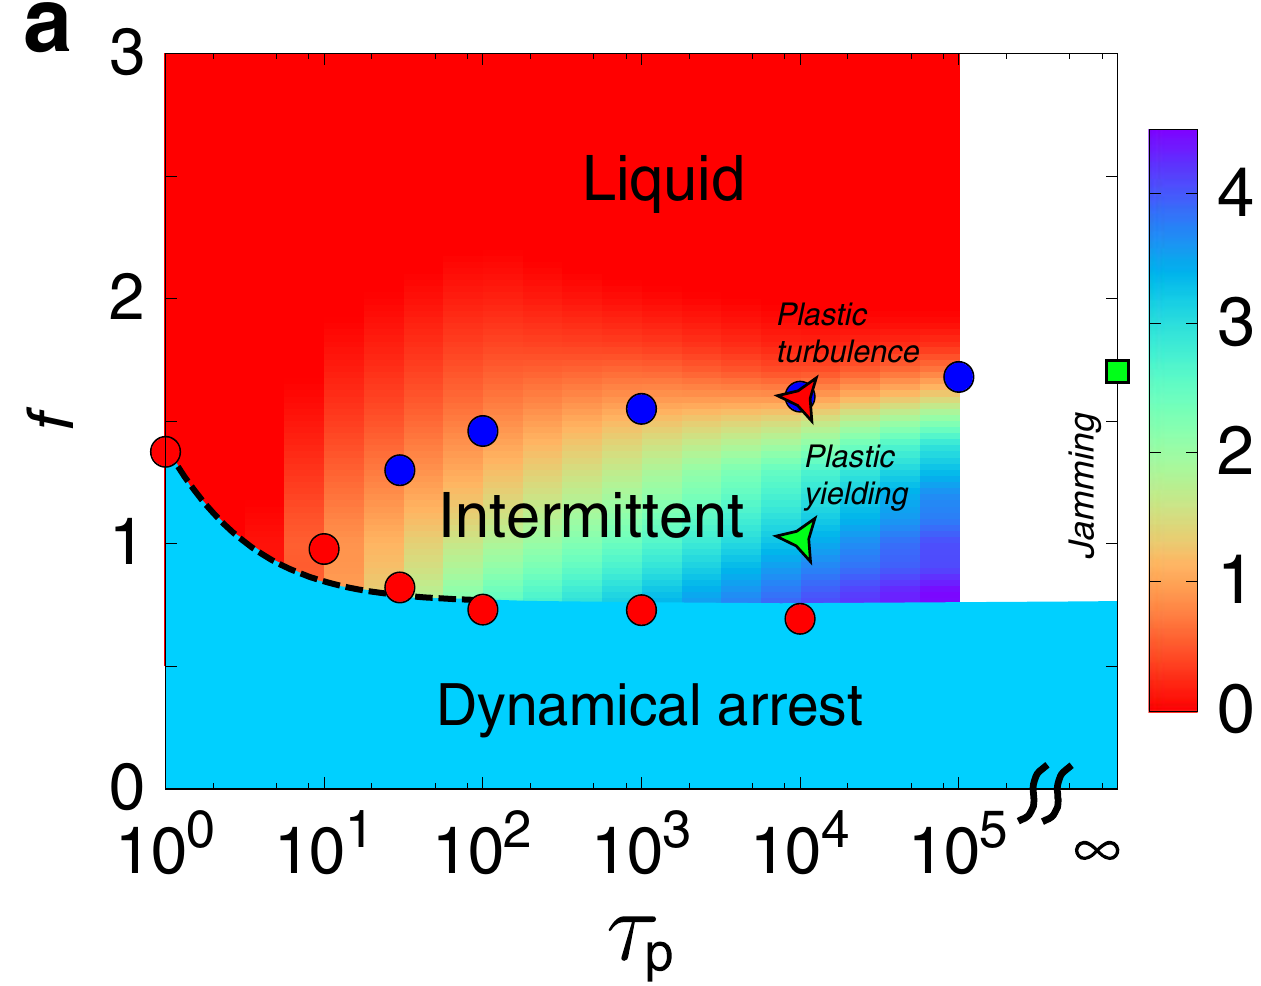
\includegraphics[height=4cm]{mandal2020_fig1a.png}
\includestandalone[height=4cm]{diagram}
\caption{{\bf (left)} Phase diagram for ABPs at fixed $\phi$ \FigureFrom{mandal2020extreme}{1(a)}. {\bf (right)} Provisional phase diagram for AOUPs at fixed $D$.}
\end{figure}

\end{frame}

\begin{frame}{Theoretical velocity correlations}

\begin{figure}
\centering
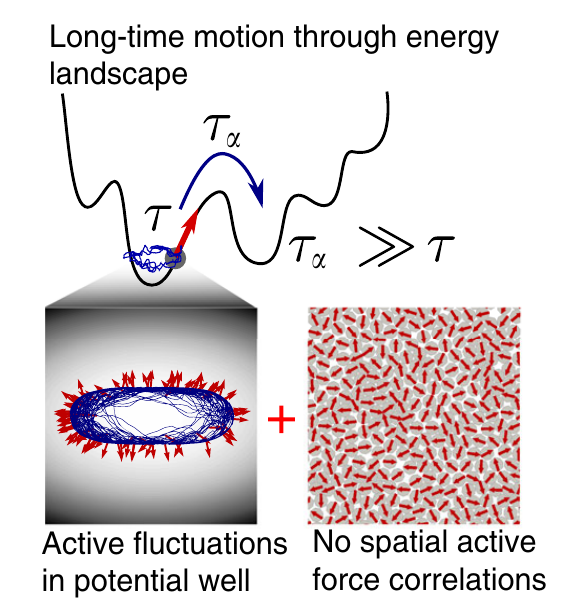
\includegraphics[height=2.75cm]{henkes2020_fig1a.png}
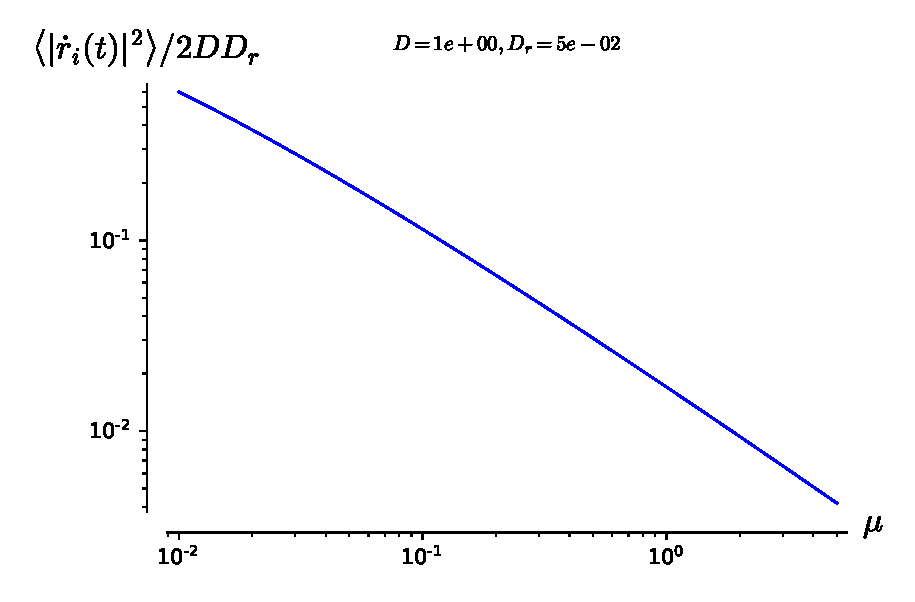
\includegraphics[height=2.75cm]{henkes_natcomm_2020_eq11.eps}
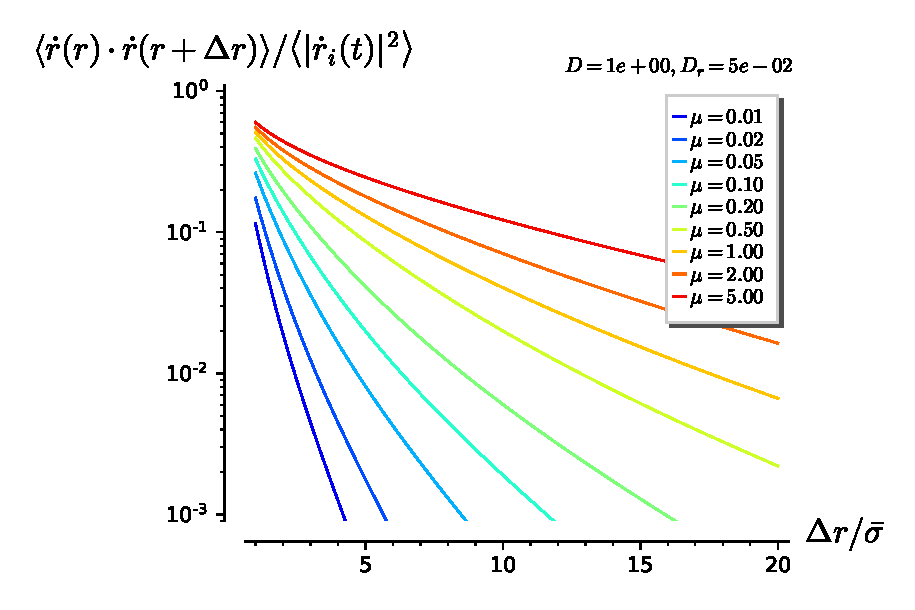
\includegraphics[height=2.75cm]{henkes_natcomm_2020_eq62.eps}\\
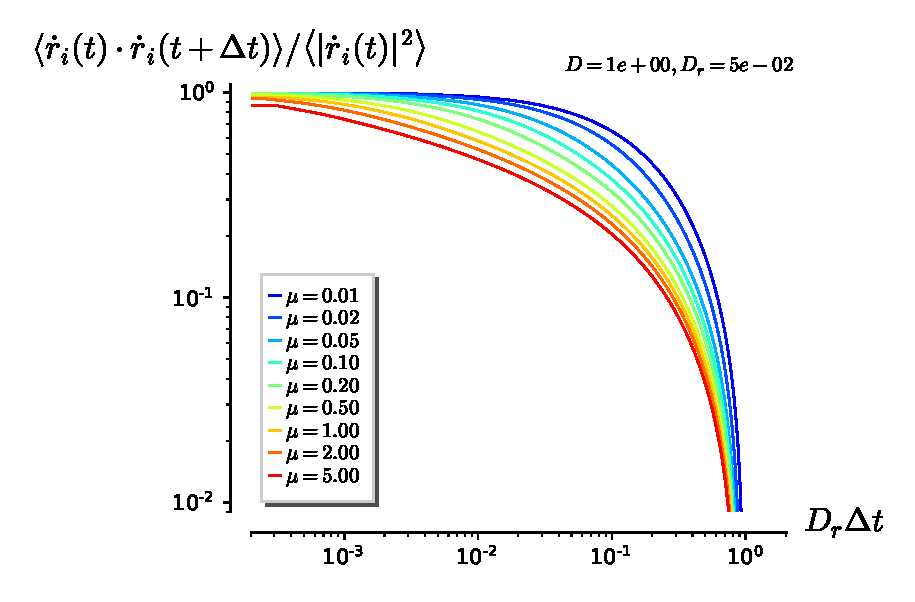
\includegraphics[height=2.75cm]{henkes_natcomm_2020_eq57.eps}
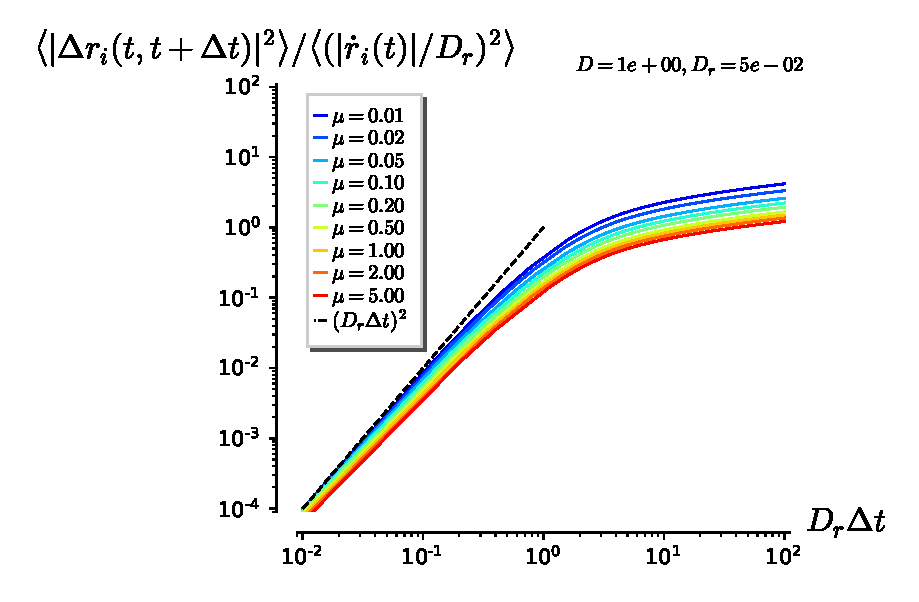
\includegraphics[height=2.75cm]{henkes_natcomm_2020_eq57_msd.eps}
\caption{{\bf (top left)} Active elastic theory \FigureFrom{henkes2020dense}{1(a)}. {\bf (top centre)} Mean squared velocity. {\bf (top right)} Radial autocorrelation function of velocity. {\bf (bottom left)} Temporal autocorrelation of velocity. {\bf (bottom right)} Mean squared displacement.}
\end{figure}

\vspace{-10pt}
\footfullcitenomark{szamel2021long}

\end{frame}

\end{document}
